\documentclass[11pt,twocolumn]{article}
\usepackage{placeins}
\usepackage[margin=0.85in]{geometry}
\usepackage{fontspec}
\usepackage{amsmath,amsthm,amssymb}
\usepackage{graphicx}
\usepackage{booktabs}
\usepackage[authoryear,round]{natbib}
\usepackage{microtype}
\usepackage{caption}
\usepackage{url}
\usepackage[hidelinks]{hyperref}
\providecommand{\tightlist}{\setlength{\itemsep}{0pt}\setlength{\parskip}{0pt}}

\title{The Fresh Protocol: A Decentralized Architecture for Trust Measurement and Validation}
\author{Devon Shigaki~(ORCID: 0009-0003-8977-8010)\\
\small The FreshCredit Lab --- Independent Research\\
\small Correspondence: freshcredit.xyz}
\date{}

% --- Float-page layout tuning: reduce white bands on float-dense pages ---
\renewcommand{\topfraction}{0.85}
\renewcommand{\bottomfraction}{0.70}
\renewcommand{\textfraction}{0.10}
\renewcommand{\floatpagefraction}{0.60}
\renewcommand{\dbltopfraction}{0.80}
\renewcommand{\dblfloatpagefraction}{0.55}
\setcounter{topnumber}{3}
\setcounter{bottomnumber}{2}
\setcounter{totalnumber}{5}
\raggedbottom


\begin{document}
\twocolumn[{\maketitle
\begin{abstract}
Institutions that measure trust --- identity providers, platforms, data
brokers, credentialing systems --- do so through centralized,
expropriative architectures whose observation of users distorts the very
behavior being measured. This paper specifies The Fresh Protocol (TFP),
a domain-agnostic, decentralized architecture for trust measurement: a
five-layer stack that implements the companion theory's stability
law (\(\Delta S_t = \lambda(V_t - E_t)\), with
\(\varepsilon_t = V_t - E_t\) the signed validation-minus-expectation
mismatch) as a live computational process, in which any verifiable
interaction --- a transaction, a credential check, an API call, a device
attestation --- functions as a validation event that updates a
user-owned record: trust measurement where genuine vulnerability is at
stake; verification/reputation measurement otherwise (\S{}1.1). The stack combines W3C decentralized
identifiers with selective-disclosure credentials (SD-JWT, IETF RFC
9901), database-per-tenant edge storage (libSQL; single-writer in
production), a Substrate settlement and audit layer (143,343 batch
transactions per second measured on 23 of 100 Kusama cores in the
December 2024 ``Spammening'' stress test; ordinary peer-to-peer
transfers peaked at 10,920 TPS), light-client verification (Smoldot),
and x402 micropayment rails (Coinbase-incubated, May 2025; 169M payments
in year one (memecoin-inflated; sub-cent settlement is the claim); zero
protocol fees; sub-cent settlement). TFP contains no
domain logic: an application is constructed by configuring the
protocol's estimator interface for a domain-specific event stream and
loading matrix (the financial application is specified in a separate financial application preprint; no financial content appears in this paper beyond minimal pointers). The protocol's defining design constraint is
measurement-theoretic: centralized observation measurably distorts the
observed (chilling effects; demand characteristics), so measurement must
be user-owned, locally verifiable, and minimally expropriative. Two boundaries are stated up front and defended in the body: (i)
user-owned measurement reduces observation salience but does not
eliminate distortion --- the protocol's own measurement still perturbs
the mismatch process (\(\psi \to \psi_{\min} < 0\), not 0; §4); and (ii)
database-per-tenant custody converts rare-catastrophic loss into
frequent-small loss --- a variance reduction whose expected-loss
advantage is conditional on endpoint hygiene and client integrity,
quantified in §3.9. All performance figures are measurements of existing
external systems cited to source, or clearly labeled simulations; cost,
speed, and security figures are printed as frozen snapshots, with the
live versioned calculator at freshcredit.xyz/cost maintained as a
supplementary tool, not a reference.
\end{abstract}
\noindent{\small\textbf{Keywords:} trust measurement; decentralized identity; verifiable credentials;
Substrate; x402; chilling effects; edge computing}
\vspace{1.5em}}]
\medskip
\noindent\textbf{Contents}\\[3pt]
{\small\noindent
1. Introduction: Trust Measurement as Infrastructure\\
2. Design Principles from the Theory\\
3. Architecture\\
4. Observation Distortion as an Engineering Constraint\\
5. Protocol Evolution and Benchmarking\\
6. Discussion\\
7. Conclusion\\
}
\medskip



\FloatBarrier
\section*{1. Introduction: Trust Measurement as
Infrastructure}

\subsection*{1.1 The problem}

Every digital interaction of consequence passes through a measurement
--- proving identity, establishing reputation, presenting a
credential, demonstrating a history --- that is trust measurement where
genuine vulnerability is at stake; verification/reputation measurement
otherwise. The incumbent measurement
infrastructure shares a common architecture --- centralized
custodianship of behavioral data --- and a common failure profile:

\begin{itemize}
\tightlist
\item
  \textbf{Compromise at scale.} In 2021, 23.9 million U.S. residents
  ($\sim$9\% of the population age 16+) experienced identity
  theft \citep{bjs2023}. U.S. data breaches generated 1.367 billion
  victim notices in 2024 (the restated figure; the Identity Theft
  Resource Center revised its initial 1.73 billion estimate downward
  after de-duplication), still up more than 300\% year over year, with
  six ``mega-breaches'' --- four of them preventable with MFA/passkeys
  --- accounting for the large majority \citep{itrc2025}. Centralized
  behavioral databases are single points of catastrophic failure by
  construction; the canonical quantification is Equifax 2017 --- 147.9
  million records, 44\% of the U.S. population, one unpatched server,
  total costs exceeding \$1.4B \citep{ftc2019}. In the language this
  paper develops below, a mass breach is an extreme injection of
  \emph{observation noise and expropriation} into the measurement
  channel: the records of millions are observed by an adversary who was
  never a party to the measurement.
\item
  \textbf{Attestation failure.} Centralized attestation is expensive and
  still does not verify reliably: the strongest cost accounting comes
  from financial-services studies --- \$5.75 in total cost per \$1 of
  fraud losses \citep{lexisnexis2025}. Synthetic-identity fraud ---
  fabricated identities ``seasoned'' with months-to-years of
  manufactured payment history before a bust-out --- is documented
  qualitatively in the Federal Reserve's three-part white-paper series
  \citep{fed2019} as among the fastest-growing financial crimes in the
  U.S. (A widely circulated claim that ``95\% of synthetic identities
  pass onboarding undetected,'' attributed to Thomson Reuters across
  vendor blogs, has no locatable primary source, methodology, or date;
  we treat it as an unverifiable industry statistic and do not rely on
  it.)
\item
  \textbf{Observation distortion.} Awareness of surveillance measurably
  changes measured behavior: after the June 2013 surveillance
  revelations, traffic to privacy-sensitive Wikipedia articles fell by a
  statistically significant $\sim$19\% immediately, with a
  persistent downward trend change (interrupted time-series design;
  \citealp{penney2016}). Experimental demand characteristics show
  heterogeneous, bidirectional participation effects with frequent nulls
  --- 12 of 19 studies positive, 5 clear nulls; the review concludes
  little is securely known about conditions, mechanisms, or magnitudes
  \citep{mccambridge2014}. A
  measurement system that frightens its subjects measures their fear.
\item
  \textbf{Stale feedback.} Institutional trust records update on
  custodial schedules --- monthly, quarterly, or upon dispute --- so the
  measurement systematically describes the past.
\end{itemize}

A scope boundary is stated up front: vulnerability-free verifiable
events (credential checks, device attestations) yield a
verification/reputation state, not trust dynamics in the theory's sense
(companion theory preprint, §1.2b, Rousseau boundary: no genuine vulnerability, no trust
dynamics); the trust reading applies only where risk and interdependence
are present.

\subsection*{1.2 The theoretical
diagnosis}

The companion theory preprint identifies the parameter that governs how expensive trust is to maintain: the
corrective bandwidth \(\mu\), the rate at which expectation--validation
mismatches \(\varepsilon_t = V_t - E_t\) are dissipated by honest,
immediate feedback. In the theory's \((S, \varepsilon)\) dynamics, the
phase volume of the mismatch flow contracts uniformly at rate \(\mu\)
(the divergence of the stated flow is the constant \(-\mu\); no critical
point or bifurcation exists in the single-agent dynamics, and none is
claimed). Centralized custodians minimize \(\mu\) --- feedback is slow,
opaque, and adversarial --- so mismatch accumulates: the stationary
variance of the mismatch process is \(\sigma^2/2\mu\), and low-\(\mu\)
regimes carry a permanently noisier alignment. And because their
observation is expropriative and unaccountable, they trigger the
measurement-dependence that the theory formalizes through the
observation-salience-dependent dissipation coefficient \(\psi\) (defined
precisely in §4 below): the act of measuring lengthens the memory of
mismatch (autocorrelation time \(1/(\mu+\psi)\)) and inflates its
stationary variance (\(\sigma^2/(2(\mu+\psi))\)). The architectural
remedy is motivated by the model rather than derived from it --- the
\(\psi\) model contains no term that ranks user-owned over
accountable-centralized observation: measurement should be user-owned,
locally
verifiable, immediately fed back, and minimally expropriative --- with
the quantified caveat, developed in §4, that this minimizes \(\psi\) but
does not drive it to zero.

Two failure registers should be distinguished explicitly, because they
have different remedies. The instrumental (logical) failures of the
incumbent stack --- error rates, stale updates, custody concentration
--- are correctness problems, addressable by better instruments. The
behavioral (psychological) failure --- observation distortion --- is not
a correctness problem: no improvement in accuracy removes it, because
its mechanism is the subject's awareness of being measured, not the
measurer's error. The incumbent failure profile above therefore
decomposes into instrumental failures (compromise, attestation,
staleness) that better engineering could in principle mitigate, and a
behavioral failure (distortion) that only an architectural change ---
non-expropriative, accountable, user-owned observation --- can address.
TFP is specified against both registers, but the second is the one the
incumbent architecture cannot retrofit.

\subsection*{1.2.1 Historical placement: what the protocol's primitives
make
possible}

The protocol sits at a specific point in the engineering lineage of the
web, and the placement is definitional rather than rhetorical. Each
regime of the web is individuated by the operation primitive it adds.
Web1 provided read: access to published data. Web2 added write: users
authored content, with the platform retaining custody of what they
wrote. The third regime adds store: user-side persistence of state,
held by the user and anchored against retroactive alteration, outside
any platform's custody (read / write / store). The operative definition
of the third regime --- independent of any asset class or product built
on top of it --- is therefore operational, not ideological: it names a
new primitive in the vocabulary of what a participant can do with data,
not a slogan. In particular, ``ownership'' is not the primitive;
ownership is the functional consequence of the store primitive --- of
who holds the state and who holds the means to alter or revoke it ---
and it obtains only where the primitive is actually implemented. What
distinguishes store from an ordinary local file is the anchoring
guarantee: consensus mechanisms, whether more or less centralized in
operation, must guarantee that stored state cannot be retroactively
altered. Decentralization is one instrument for securing that guarantee;
it is the guarantee itself that constitutes the capability shift. The
historical analogy is asymmetric-key cryptography: RSA did not create
any new class of application --- communication, commerce, and identity
all predated it --- but it made those applications securable without a
shared secret, and every secure channel since is built on that unlock.
User-side anchored storage occupies the same position for measurement
infrastructure: it adds no new domain capability, but it makes an
existing one --- continuous, high-resolution trust measurement ---
possible without custodial exposure, which is the precondition for
everything this paper specifies. The placement also counters a recurring
industry narrative that conflates capability with scale: the read
\(\to\) read/write \(\to\) read/write/store progression is a capability
sequence, and the decisive step is store (anchored, user-held state),
not any increment of throughput. Scale is an engineering consequence of
execution architecture (§3.4); capability is what the primitive unlocks.
This distinction is why the choice of chain is load-bearing rather than
cosmetic.

\subsection*{1.3 Scope: the protocol, not an
application}

TFP is deliberately agnostic about what is being validated. It supplies:
identity primitives, user-owned data topology, a validation compute
layer applying the stability law, a settlement/audit substrate, and
governance-by-design (user-owned custody, accountable access logging,
open standards --- see §3.5 for what this does and does not include). It
does not contain scoring models, credit logic, financial regulations, or
any domain-specific decision rules. Applications consume the protocol's
validation stream and impose their own domain semantics; the financial application preprint (specified separately) applies this protocol to finance, including all credit-pull, bureau, and
scoring content. This separation is architectural hygiene: the
protocol's claims must stand on infrastructure evidence, not on any one
application's regulatory or predictive record.

\subsection*{1.4 Hypotheses and proof
obligations}

The hypothesis below matches the tested design (§3.6) and is the
registered form (specified and timestamped in the Supporting Document;
an OSF registration of the same design filed with the deposit (DOI: [insert]) prior to any pilot data collection).

\textbf{Null hypothesis (H0).} Feedback coupling has no effect on
population-level trust-field coherence (the Kuramoto order parameter R
stays at the finite-size incoherent floor \(\approx\) \(1/\sqrt{N}\) at
all coupling strengths), observation leakage has no effect on coherence
at fixed coupling, and edge architecture does not reduce the marginal
cost of engagement.

\textbf{Alternative hypothesis (H1).} Three legs, stated in the
direction actually tested:

\begin{enumerate}
\def\labelenumi{\arabic{enumi}.}
\tightlist
\item
  \textbf{Coupling produces coherence.} Under protocol feedback coupling
  at sufficient strength K, the agent population self-organizes above
  the coherence threshold (target: order parameter \(R > 0.7\)); the
  isolated control (\(K = 0\)) remains at the incoherent floor (target:
  \(R < 0.3\)). Coherence is a property of the coupling --- of the
  feedback composition --- not of isolated stores.
\item
  \textbf{Observation leakage degrades coherence.} At fixed K, R decays
  monotonically as the observation-leakage parameter \(\ell\) rises
  (operationalized exactly in §3.6). The architectural content of the
  privacy claim lives here: non-expropriative measurement is what keeps
  \(\ell\) below the fragility threshold at which coherence collapses.
\item
  \textbf{Edge architecture reduces marginal cost.} Edge compute plus
  per-event micropayment settlement achieves a marginal cost per
  validation event far below incumbent marginal per-query costs,
  stated as a conditional (incumbent marginal price \(>\) \$0.05/query)
  against printed frozen figures; the reduction factor itself is not
  printed (§3.6, Sim P3; §5.2).
\end{enumerate}

The protocol's proof obligations: (1) an agent-based simulation of
coupled vs.~isolated conditions --- run and reported in §3.6 against
pre-registered criteria, with an OSF registration of the same design filed with the deposit (DOI: [insert]) prior to any pilot data collection --- with coherence differences evaluated at \(p < 0.001\);
(2) the leakage-graded desynchronization arm --- R(K, \(\ell\)) mapped over a
(K, \(\ell\)) grid, run and reported in §3.6 (Sim P1b); (3) the
coherence threshold itself (leg 1); (4) cost --- edge compute plus
x402-class settlement at near-zero marginal per-validation cost, with
the comparison restricted to like-for-like marginal quantities and
frozen figures printed in §5.2. Obligations (1), (2), and (3) are now
discharged in silico in §3.6, \textbf{with an honest null on the
quantitative threshold}: leg 1 is supported (\(R = 0.739\) \(\pm\) 0.029
coupled vs.~\(0.040 \pm 0.001\) isolated --- the verification re-run
values; the isolated arm sits at the \(1/\sqrt{N}\) \(\approx\) 0.045
finite-size floor); leg 2 is supported qualitatively (R decays
monotonically in \(\ell\) at every K tested --- mechanism demonstrated
in silico under a stated operationalization whose attenuation component
is definitional; \S3.6) but the zero-leakage
operating point \(K = 4.5\) is fragile --- R falls below the 0.7 target
within the leakage band \(\ell\)* \(\in\) {[}0.02, 0.10{]} (a 9-seed
fine scan at \(K = 4.5\) gives R \(\approx\) 0.69--0.74 across \(\ell\)
\(\in\) {[}0, 0.10{]}, first below-0.7 reading at \(\ell = 0.08\); the
exact crossing is not resolvable at seed noise \(\pm 0.02–0.03\)), so
robust \(R > 0.7\) requires either stronger coupling or a lower
coherence target --- at \(K = 6\) coherence survives to \(\ell \approx
0.22\text{--}0.28\) and at \(K = 8\) to \(\ell \approx
0.30\text{--}0.40\) (ranges span two independent seeded re-renders;
point precision is not resolvable at these N). Obligation (4) is
restated in like-for-like form and maintained against printed frozen
figures plus the supplementary versioned calculator; it is not asserted
as a deployed result.

\subsection*{1.5 Epistemic posture}

All quantitative figures in this paper are (a) measurements of existing
external systems, cited to source; (b) labeled simulations over
synthetic data; or (c) frozen benchmark snapshots printed in §5.2, with
the live, versioned calculator at freshcredit.xyz/cost maintained as a
supplementary tool --- the print figures, not the live page, are the
canonical reference for this paper's claims. No achieved end-to-end
performance is claimed for deployed applications of the protocol. Claims
carry the stack's epistemic labels: \textbf{{[}DERIVED{]}} (follows from
stated assumptions), \textbf{{[}STANDARD{]}} (textbook results derived
for self-containment), \textbf{{[}ANALOGY{]}}, \textbf{{[}HOMOLOGY{]}},
\textbf{{[}EMPIRICAL{]}}, \textbf{{[}HYPOTHESIS{]}},
\textbf{{[}SIMULATION{]}}.


\FloatBarrier
\section*{2. Design Principles from the
Theory}

Three principles follow from the theory and biology layers of the stack (the companion theory and biological-instantiation preprints):

\begin{enumerate}
\def\labelenumi{\arabic{enumi}.}
\item
  \textbf{Interactions as validations (theory layer).} Any event with a recorded
  expectation and a recorded outcome can drive the stability update.
  Stack-wide, the update is the master law

  \begin{equation}\begin{split} S_{t+1} ={}& S_t + \lambda^{+}\max(\varepsilon_t, 0)\,r_t + \lambda^{-}\min(\varepsilon_t, 0)\,r_t \\ & - \delta_S\,(S_t - S_{\mathrm{base}}), \qquad \varepsilon_t = V_t - E_t, \end{split}\label{eq:master} \end{equation}

  with \(\lambda^{+}\), \(\lambda^{-}\) \(\geq 0\) the
  confirmation/betrayal sensitivities, \(r_t\) \(\in\) {[}0,1{]} the
  recognition gate, \(\delta_S\) \(\geq 0\) the retention leak, and
  \(S_{\mathrm{base}}\) the baseline; \(\varepsilon\) is dimensionless
  after per-domain normalization (\(\tilde{\varepsilon}\) = (V \(-\)
  \(E)/s_d\), \(s_d\) the RMSE of the domain's expectation distribution,
  companion theory preprint, Def. 2a). The named layer presets are: the physics layer
  (\(r = 1,\) \(\delta_S = 0,\) \(\lambda^{+} = \lambda^{-} = \lambda\)
  --- the Rescorla--Wagner limit, reducing exactly to
  \(\Delta S_t = \lambda (V_t\) \(-\) \(E_t\))); the biological
  layer (gating \(r_t\), baseline-restoring leak \(\delta_S > 0,\)
  \(S_{\mathrm{base}}\) the homeostatic prior); and the \textbf{TFP
  protocol layer (\(\lambda^{-} > \lambda^{+}\) --- break/build
  asymmetry: betrayal updates faster than confirmation accrues --- as an
  explicitly labeled extension)}, with \(r_t \equiv 1\) and \(\delta_S\)
  \(\geq 0.\) The protocol therefore treats validation as a primitive: a
  typed, timestamped, attributable event with an expectation field and
  an outcome field. Domains differ only in what fills those fields.
\item
  \textbf{The five-channel measurement (biology).} Interaction streams ---
  behavioral, transactional, physiological --- are measurement layers on
  the same latent trust process, scored against the frozen biological stage
  mapping (D--O--C--A--S). The protocol records streams; the companion biology
  experiment interprets them; applications decide which streams they
  consume and for what. Streams with decision-ethical sensitivity (e.g.,
  physiological data) are sequestered at the schema level from
  application decision paths.
\item
  \textbf{Distortion-minimizing observation (measurement theory).} Data
  minimization (selective disclosure), ownership locality
  (database-per-tenant), local verification (light clients), and
  accountable observation (user-visible, on-chain access logs) are the
  engineering responses to the documented chilling and
  demand-characteristic distortions of §1.1. Stated against the
  now-defined \(\psi\) (§4): these four responses drive observation
  salience m toward its floor, and hence
  \(\psi \to \psi (m_{\mathrm{min}})\) --- which the theory and the
  \(\psi\) battery (§4) both say is \textbf{negative and nonzero}: the
  protocol's own measurement still distorts, and §4 applies a
  Campbell's-law caution to the protocol's own metrics accordingly.
\end{enumerate}


\FloatBarrier
\section*{3. Architecture}

The components are existing, production-grade open systems; the
contribution is their composition into a trust-measurement loop.
Figure~\ref{fig:stack} summarizes the reference architecture as a
five-layer stack of mathematical objects, with the core flow and the
cross-cutting population-level objects drawn outside the layers because
no single layer owns them.

\begin{figure*}[!tp]
\centering
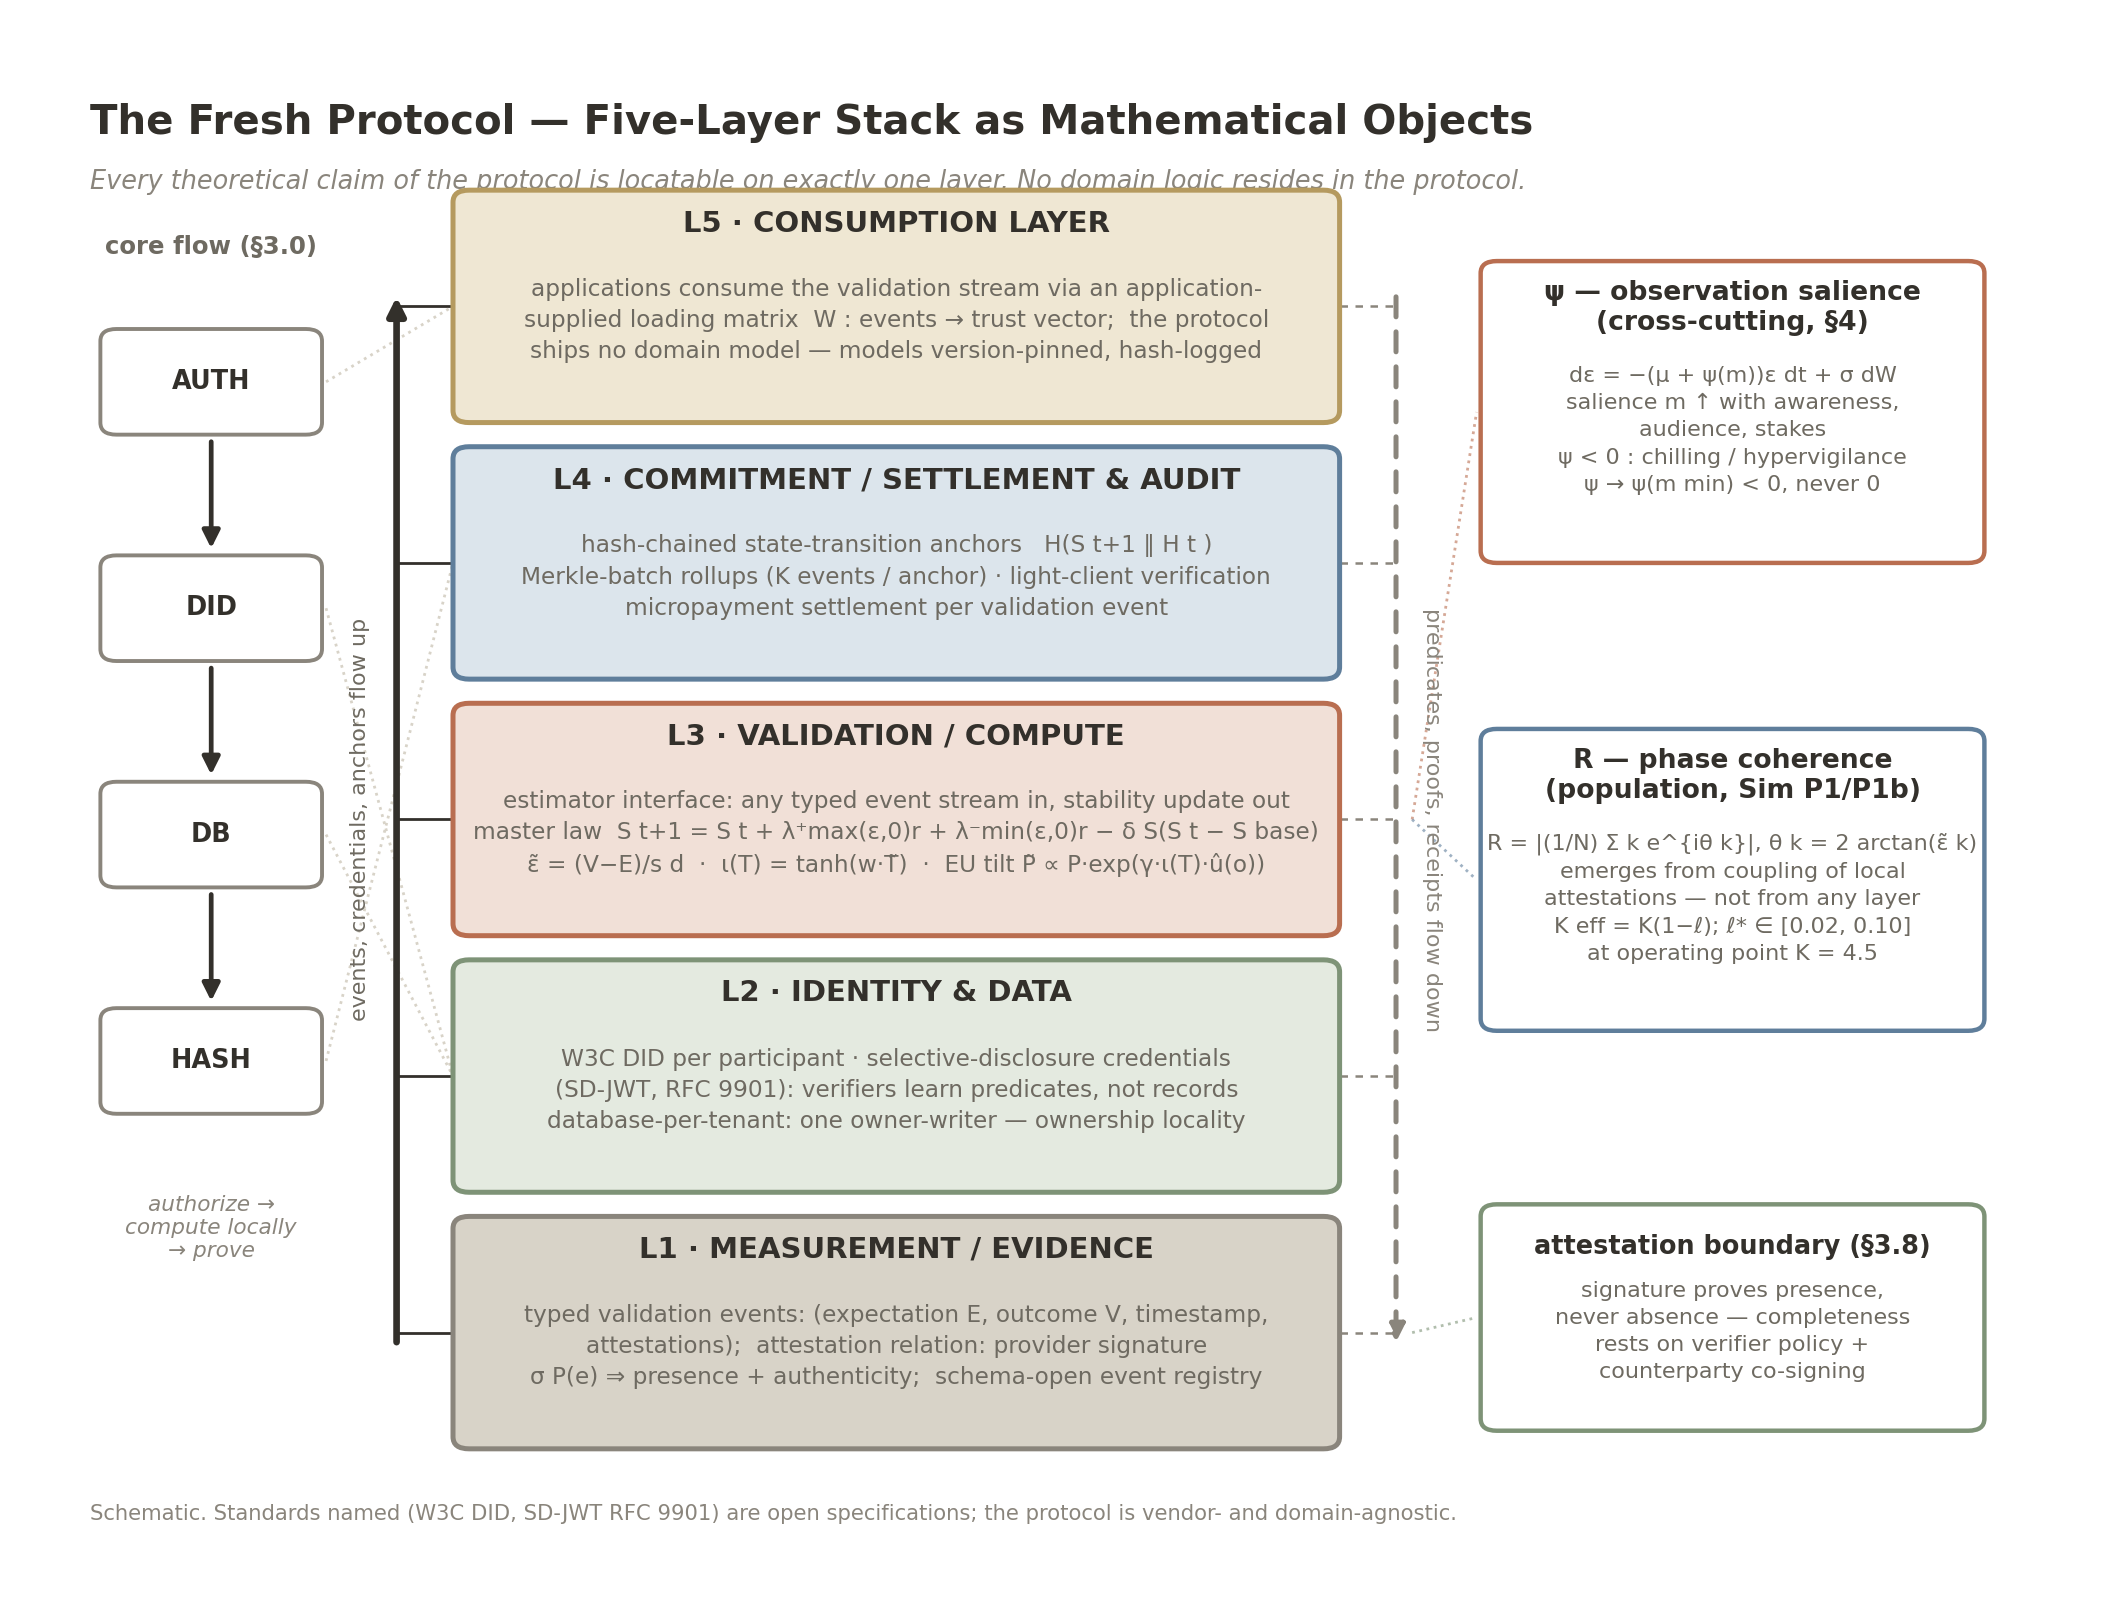
\includegraphics[width=0.92\textwidth]{figures/tfp_protocol_stack.png}
\caption{The Fresh Protocol as a five-layer stack of mathematical objects (\S3 opening). L1 measurement/evidence: typed validation events ($E$, $V$, timestamp, attestations) and the provider-signature attestation relation (presence + authenticity). L2 identity \& data: W3C DIDs, selective-disclosure credentials (SD-JWT, RFC 9901 --- predicates, not records), database-per-tenant ownership locality. L3 validation/compute: the estimator interface, the master law (TFP preset $\lambda^{-} > \lambda^{+}$), $\tilde{\varepsilon}$ normalization, the $\iota(T)$ trust index and the bounded exponential-tilt $\mathrm{EU}(a \mid T)$. L4 commitment/settlement \& audit: hash-chained state-transition anchors, Merkle-batch rollups, light-client verification, per-event micropayment settlement. L5 consumption: applications via an application-supplied loading matrix; no domain logic in the protocol. The core flow AUTH $\to$ DID $\to$ DB $\to$ HASH (left rail) and the cross-cutting/population-level objects $\psi$ (observation salience), $R$ (phase coherence), and the attestation boundary (right rail) are drawn outside the layers because no single layer owns them.}
\label{fig:stack}
\end{figure*}

\subsection*{3.0 The core flow}

Every interaction with the protocol traverses a single sovereign
pipeline:

\textbf{AUTH \(\to\) DID \(\to\) DB \(\to\) HASH}

AUTH --- the participant authenticates to their own edge environment
(device-held keys); no custodial account exists to be breached. DID ---
the participant's decentralized identifier scopes the interaction;
credentials are presented by selective disclosure (predicates, not
records). DB --- the validation event is written to the participant's
own database-per-tenant store; the stability update
\(\Delta S = \lambda (V\) \(-\) E) (TFP preset:
\(\lambda^{-} > \lambda^{+}\) asymmetric form, §2) is computed at the
edge, so raw data never leaves the participant's control. HASH --- the
resulting state transition is hashed to the audit chain, giving the
participant --- and only parties they authorize --- a
light-client-verifiable proof of record integrity. The pipeline is the
architectural negation of the custodial flow it replaces: where the
incumbent pattern is collect \(\to\) centralize \(\to\) expose, the
protocol's is authorize \(\to\) compute locally \(\to\) prove.
Figure~\ref{fig:evflow} renders the expectation--validation loop the
pipeline carries --- one signed mismatch per event driving one state
update, closed through the trust index --- and where the audit and
observation terms attach.

\begin{figure*}[!tp]
\centering
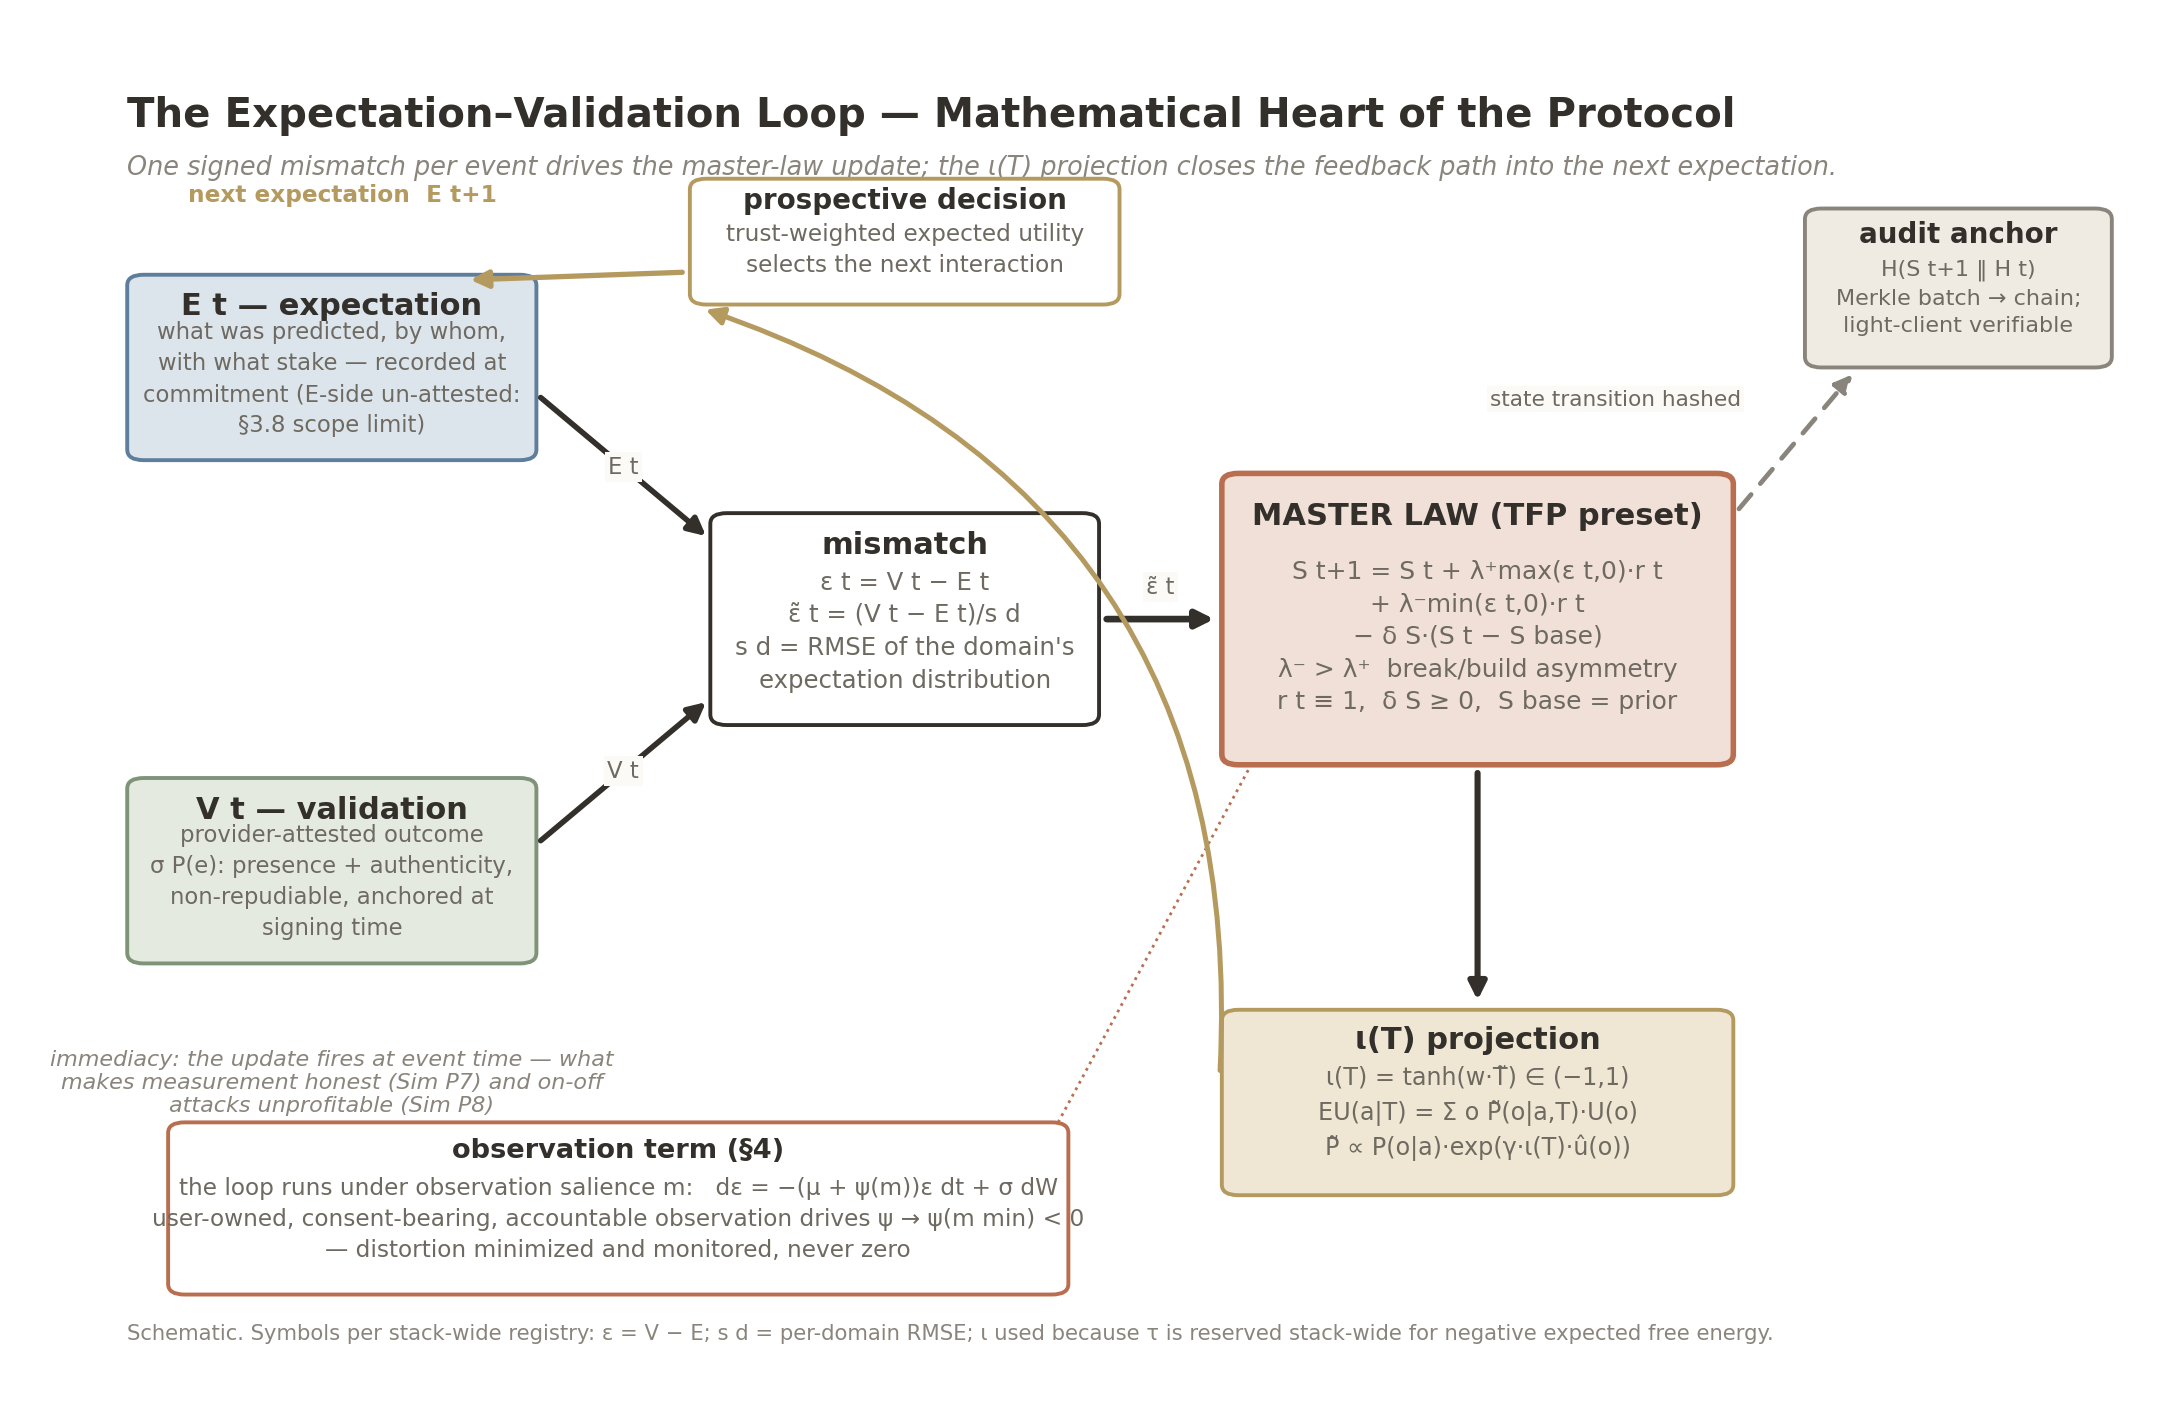
\includegraphics[width=0.92\textwidth]{figures/tfp_ev_dataflow.png}
\caption{The expectation--validation loop (\S3.0--3.3). A recorded expectation $E_t$ and a provider-attested outcome $V_t$ form the normalized mismatch $\tilde{\varepsilon}_t = (V_t - E_t)/s_d$, which drives the master-law update $S_{t+1} = S_t + \lambda^{+}\max(\varepsilon,0)r + \lambda^{-}\min(\varepsilon,0)r - \delta_S(S_t - S_{\mathrm{base}})$ with the TFP preset $\lambda^{-} > \lambda^{+}$ (break/build asymmetry), $r \equiv 1$, $\delta_S \geq 0$. The state projects through $\iota(T) = \tanh(w \cdot \tilde{T})$ into trust-weighted expected utility (exponential tilt $\tilde{P} \propto P \cdot \exp(\gamma\,\iota(T)\,\hat{u}(o))$), which selects the next interaction and thereby the next expectation --- the feedback path. Every state transition is hashed to the audit anchor. The observation term ($d\varepsilon = -(\mu + \psi(m))\varepsilon\,dt + \sigma\,dW$) is annotated as the regime the loop runs under; the $E$-side is marked un-attested (\S3.8 scope limit).}
\label{fig:evflow}
\end{figure*}

\subsection*{3.1 Measurement layer}

Validation events enter as typed records: expectation (what was
predicted, by whom, with what stake), outcome (what occurred),
timestamp, and attestations. Sources are arbitrary: signed API
responses, credential presentations, device attestations, settlement
receipts, consented wearable streams. The layer is schema-open --- new
domains register event types without protocol changes. Attestation is
the load-bearing integrity \emph{and} completeness mechanism of this
layer; §3.8 states precisely what a provider-signed event proves
(presence and authenticity) and what it cannot prove (absence of omitted
events), and what the protocol does about the gap. The scope boundary of
§1.1 binds the layer's outputs: vulnerability-free verifiable events
(credential checks, device attestations) yield a verification/reputation
state, not trust dynamics in the theory's sense (companion theory preprint, §1.2b, Rousseau
boundary: no genuine vulnerability, no trust dynamics); the trust
reading applies only where risk and interdependence are present.

\subsection*{3.2 Identity and data layer}

Each participant holds a W3C decentralized identifier (DID;
\citealp{w3c2022did}); attestations are verifiable credentials presented
by selective disclosure --- verifiers learn predicates (``over 18'',
``credential unrevoked'', ``no failed obligations in window w''), not
records. Production DID ecosystems demonstrate the pattern: KILT
Protocol --- a Substrate-based blockchain operating as a Polkadot
parachain --- provides production issue-hold-verify credential flows
(verifiable, revocable, selectively disclosable credentials anchored by
on-chain hashes) documented since its 2019 whitepaper \citep{kilt2019}.
The standards layer has since matured from draft to regulated default:
the Verifiable Credentials Data Model 2.0 reached full W3C
Recommendation status in May 2025 \citep{w3c2025vc}, and the
selective-disclosure JWT format is standardized as SD-JWT (IETF RFC
9901, a finished Standards-Track specification; \citealp{rfc9901}); its
credential profile SD-JWT VC --- still an IETF Internet-Draft, not yet
an RFC --- is mandated (alongside ISO mdoc) in the EU's eIDAS 2.0 wallet
architecture. (For the unlinkable-presentation case, BBS cryptosuites
exist but are W3C Candidate Recommendation Drafts, not yet
Recommendations; the stack does not depend on them.) Selective
disclosure is no longer a research construct; it is the direction
regulation is pulling.

Data live in a database-per-tenant topology (libSQL;
\citealp{turso2026}): each participant's trust record is an independent
encrypted edge database whose durability is provided by cloud backups or
offline backups under the participant's control. One engine fact is
stated precisely because the ecosystem's naming invites confusion: the
production libSQL engine (the C fork of SQLite that powers Turso Cloud
today) inherits SQLite's \textbf{single-writer} model; MVCC concurrent
writes are a feature of Turso's ground-up Rust rewrite of SQLite,
currently in beta, not of the production engine. Nothing in this
architecture requires concurrent writers per tenant --- each database
has exactly one owner-writer --- so the production engine suffices; the
beta rewrite is noted for trajectory only. The topology yields
local-latency I/O (vendor benchmarks report \(\sim 3\times\) improvement
over centralized round-trips) and, more importantly, ownership locality:
the record is the participant's, licensed to queries, rather than a
custodian's asset. Aggregation APIs that permission data at the source
(Plaid, Stripe, and equivalents) demonstrate the consent-bearing query
pattern at production scale --- the protocol generalizes it beyond
finance.

\begin{figure*}[!tp]
\centering
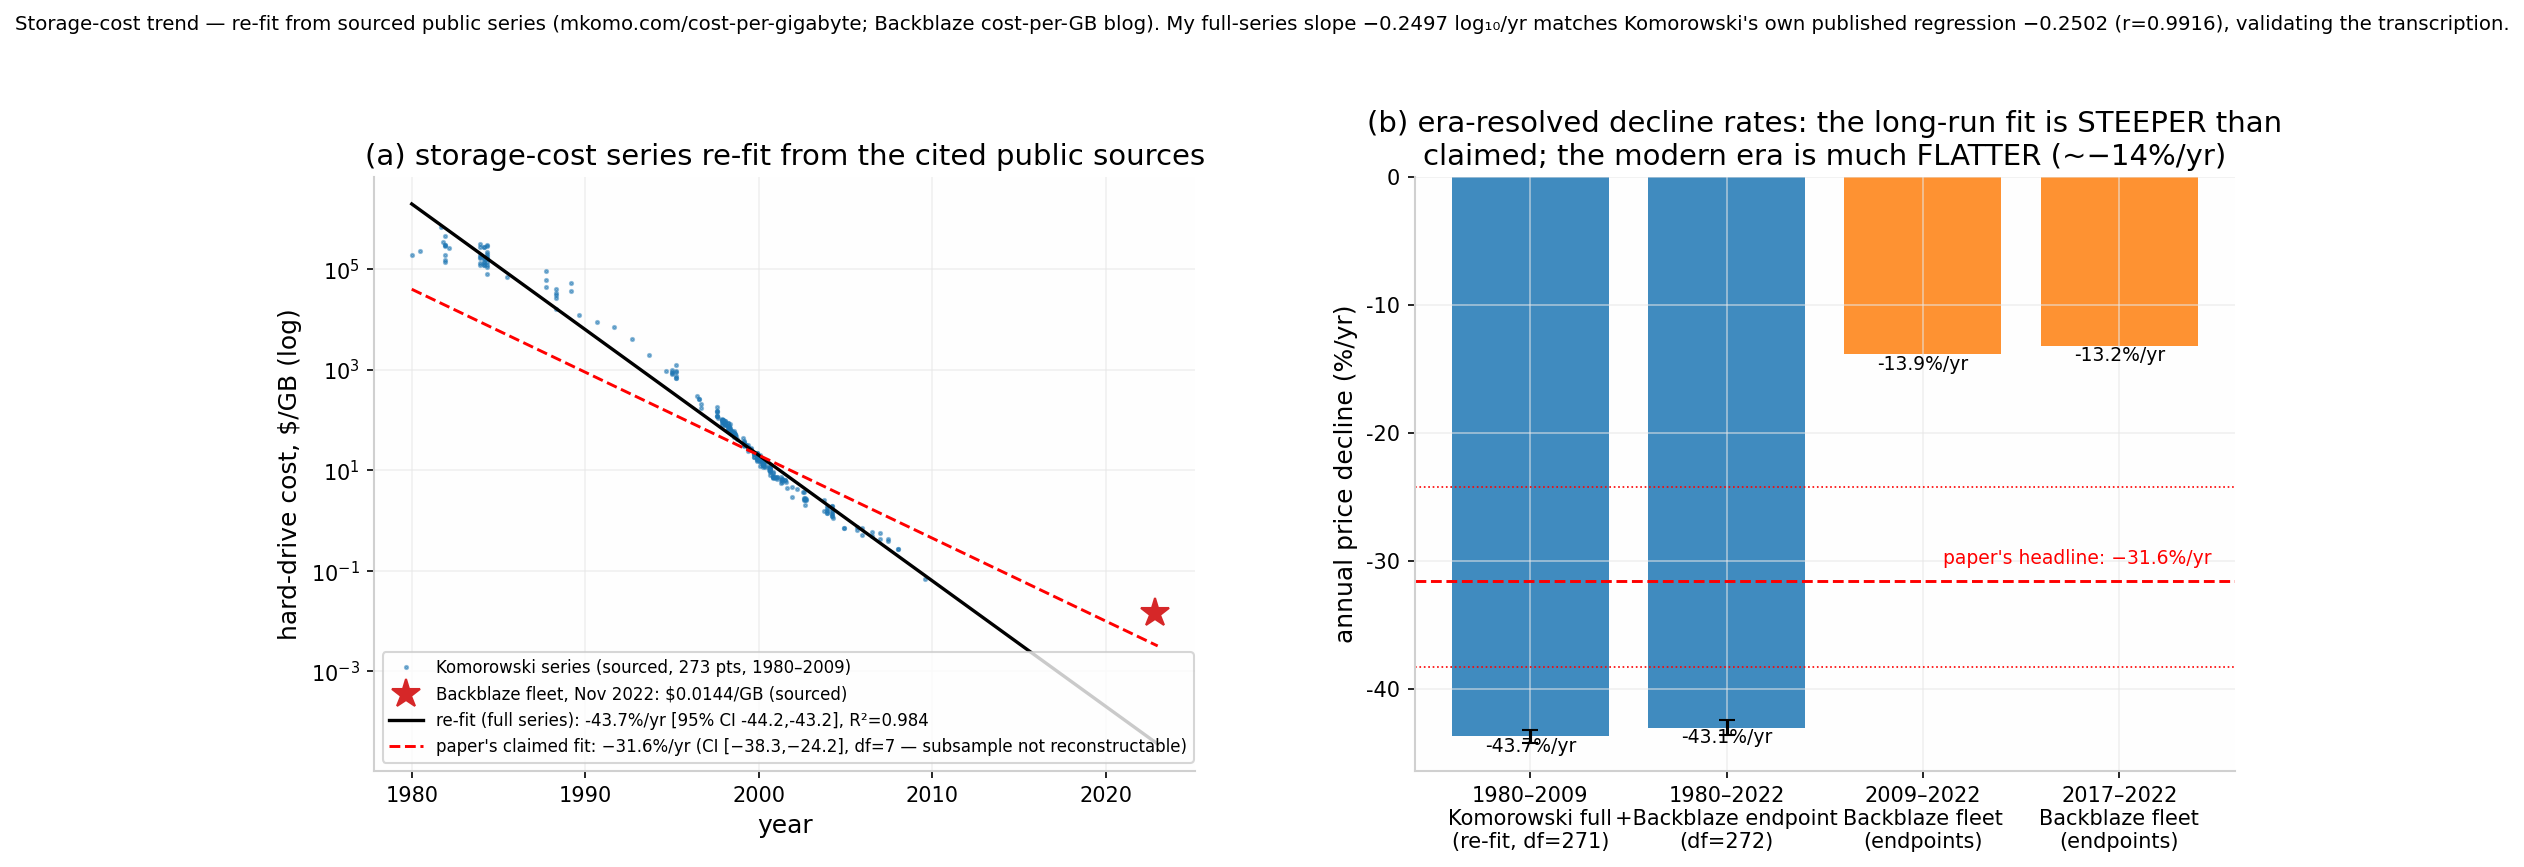
\includegraphics[width=0.92\textwidth]{figures/fig_storage_refit.png}
\caption{Storage-cost trend, era-split (\S3.2): the full sourced Komorowski table \citep{komorowski2024} (273 drive-price points, 1980--2009) re-fit log-linearly at $-43.7$\%/yr (95\% CI $[-44.2, -43.2]$, $R^2 = 0.984$), matching Komorowski's own published regression; Backblaze fleet endpoints \citep{backblaze2022} extend the series to \$0.0144/GB (November 2022) and give the much flatter modern era of $\approx -14$\%/yr. A $-31.6$\%/yr fit (df $= 7$) on a small subsample is unreconstructable from the cited series and is not used.}
\label{fig:storage}
\end{figure*}

Two properties of this layer are stated with their evidence. First, the
cost curve is measured, not asserted, and the trend is era-split (Figure
\ref{fig:storage}): a re-fit on the full sourced Komorowski table
\citep{komorowski2024} (273 transcribed drive-price points, 1980--2009)
gives a log-linear decline of \(-43.7\%/year\) (95\% CI {[}\(-44.2\),
\(-43.2\){]}; \(R^{2} = 0.984\); halving every 1.2 years), matching
Komorowski's own published regression of the same series (\(-0.250\)
\(log_{10}/yr\); \citealp{komorowski2024}), while the modern era is much
flatter --- \citeauthor{backblaze2022} fleet endpoints give \(\approx\)
\(-14\%/year\) over 2009--2022 (\$0.114/GB in 2009 to \$0.0144/GB in
November 2022, an 87\% drop). A \(-31.6\%/year\) fit on a
small subsample (df = 7) is unreconstructable from the cited series --- its
1980 anchor of ``roughly \$20,000/GB'' conflicts with the sourced
Komorowski 1980 rows (\$152K--\$700K/GB) --- and is not used; the re-fit
above is the claim, with the caveat that the 2025--26 NAND shortage reversed
SSD pricing (enterprise +257\%) while HDDs continued the trend (+35\%)
--- a 46-year pattern, not a law (storage-cost study, Supporting
Document §S.4). Declining storage cost is what makes database-per-tenant
durable history economically ordinary rather than exotic. Second,
distribution removes the incentive, not just the breach: a centralized
custodian is a honeypot whose compromise is worth \$4.44M on average
globally and \$10.22M in the U.S. per incident
\citep[customer PII present in 53\% of breaches]{ibm2025}. Perimeter
scaling answers this with more cameras and higher walls around an
ever-more-valuable target; database-per-tenant architecture deletes the
target --- there is no aggregate vault whose breach amortizes an
attacker's cost across millions of records. The expected-loss
counterpart of this static argument --- what distribution does to the
\emph{probability} side of the risk equation --- is quantified, with its
failure modes, in §3.9.

A note on zero-knowledge proofs, stated precisely because the argument
is often made badly. A ZK predicate proof over a signed credential is
definitive for the predicate it proves (a range proof on an attested
date of birth conclusively establishes ``not under 21''); what it does
not establish is the truth of the underlying attestation, which lives
outside the proof --- nor the \emph{completeness} of the attested set
(§3.8). The practical limitation is expressivity, not soundness:
predicate proofs disclose binary answers, and heterogeneous credential
logic --- professional licensure, composite standing, conditional
eligibility --- is general computation, not a fixed predicate. On-chain
general-purpose runtimes (§3.4) evaluate such verification programs
directly, with ZK reserved for the disclosure-minimizing cases where it
is strictly the right tool. Selective disclosure (SD-JWT) and predicate
proofs are complementary instruments in the stack, not rivals.

\subsection*{3.3 Validation / compute
layer}

An edge-compiled evaluation engine applies the theory's two operations
to each event: the trust-weighted expected utility for prospective
decisions, and the stability update for completed ones. Both are stated
as derived in the companion theory preprint (§2.3, Eq. (2); §M3 of the
stack's Technical Appendix --- the simulation batteries and mathematical
development cited throughout this paper, bundled in the pending
Supporting Document deposit; cited below as
``Technical Appendix, §M'' and ``Technical Appendix, Sim-Battery A/B,
Study N''):

\begin{itemize}
\tightlist
\item
  \textbf{Stability update (completed events):} the master-law TFP
  preset,
  \(S_{t+1} = S_t + \lambda^{+}\varepsilon_t^{+} + \lambda^{-}\varepsilon_t^{-} - \delta_S(S_t - S_{\mathrm{base}})\)
  with \(\varepsilon_t = V_t - E_t\) dimensionless after per-domain
  normalization and \(\lambda^{-} > \lambda^{+}\) (break/build
  asymmetry, explicitly labeled extension). Participant-level
  \(\lambda^{+}\), \(\lambda^{-}\) are estimated separately from
  positive- and negative-\(\varepsilon\) subsamples of the event history
  under the state-space estimators specified in the companion theory preprint, §6 (Kalman/EM;
  Bayesian hierarchical). The population-mean target for the symmetric
  sensitivity is pre-registered in the companion theory preprint as \(\mu_{\lambda} = 0.61\) with corridor
  {[}0.46, 0.76{]} --- a target hypothesis whose corridor half-width is
  a pre-registered smallest effect size of interest (SESOI), not a
  derived constant and not a claim of this paper.
\item
  \textbf{Trust-weighted expected utility (prospective decisions):}
  \begin{equation} \mathrm{EU}(a \mid T) = \sum\nolimits_o \tilde{P}(o \mid a, T)\,U(o), \label{eq:eu} \end{equation} where the trust index
  \(\iota(T) = \tanh(w\,\tilde{T}) \in (-1, 1)\) distorts outcome
  probabilities by a bounded exponential tilt \begin{equation} \tilde{P}(o \mid a, T) \propto P(o \mid a)\,\exp\bigl(\gamma\,\iota(T)\,\hat{u}(o)\bigr) \label{eq:tilt} \end{equation} (companion theory preprint, §2.3; the
  symbol \(\iota\) is used because \(\tau\) is reserved stack-wide for
  negative expected free energy). At neutral trust (\(\iota = 0\)) this
  is exactly standard expected utility; the distortion is bounded
  (\(|\log \tilde{P}/P| \leq 2\gamma \max|\hat{u}|\), sharp form
  \(\gamma\cdot(\max\hat{u} - \min\hat{u})\); \(2\gamma \max|\hat{u}|\)
  is the looser safe bound; the qualitative conclusions are unaffected), so trust reweights
  evidence but never manufactures outcomes. The index \(\iota(T)\) is a
  projection of the state, not the state; no single scalar is a
  sufficient statistic of the dynamics (companion theory preprint, §2.3a).
\end{itemize}

This layer is the protocol's entire contract with measurement: any
timestamped, verifiable event stream enters here, and an
application-supplied loading matrix maps the stream onto the trust
vector. Which streams an application aligns --- physiological,
financial, credential, device --- and which reference geometry it aligns
them against are the application's specification, not the protocol's;
the protocol supplies the estimator interface and the audit trail,
nothing more. The layer ships no domain model; models are
application-supplied and version-pinned, with all model versions
hash-logged for audit. (The financial application preprint, specified separately, is the worked example: it specifies the health-and-financial stream alignment that this layer
deliberately refuses to specify.) The one direct cross-domain test in
the stack (the companion biology preprint's Sim D8 multilingual arms) failed its pre-registered
criteria; domain-generality of the estimator interface is therefore an
architectural claim, not a demonstrated one.

\subsection*{3.4 Settlement and audit
layer}

State transitions of trust records are hashed to a Substrate-based
chain. The throughput evidence, stated with its transaction mix: in the
December 4, 2024 ``Spammening'' live stress test on Kusama (1,933
community participants, $\sim$30 minutes, real economic value),
the network processed \textbf{143,343 transactions per second using 23
of 100 validator cores} --- a measured figure, but for \emph{batch}
(one-to-many, airdrop-style) transactions; ordinary peer-to-peer
transfers peaked at \textbf{10,920 TPS on 15 cores} in the controlled
November 26, 2024 Parity test, and the often-quoted 623,230 TPS figure
is Parity's linear extrapolation to 100 cores, not a measurement
\citep{spammening2024}. Block rollups (K events per anchor; §3.7, Sim
P8) place per-validation anchoring comfortably inside the measured
envelope. End-user verification uses Smoldot light clients
\citep{smoldot2026}, which sync and verify block headers and finality
proofs locally in the browser or on device \emph{without trusting any
full node or RPC server} --- so any participant can audit their own
record's integrity without trusting an intermediary, the architectural
form of verifiable feedback. (No per-verification latency benchmark for Smoldot is published; no such figure is claimed here.)

\textbf{Component evidence, by evidence class.} The settlement layer's throughput figures are measured on a live network (above). The remaining layer components are cited from official documentation and vendor benchmarks, and are labeled as such: storage-layer local queries run at $\approx$200 ns with prepared statements (Turso libSQL micro-benchmark [VENDOR BENCHMARK]); the reference state-trie implementation (NOMT) commits and proves an update of 50{,}000 accounts in 1.151 s --- $\approx$43{,}000 updates/s on commodity NVMe (rob.tech benchmark [VENDOR BENCHMARK]); identity and credential components (W3C DIDs, SD-JWT, KILT-class production flows) are specified from official documentation [DOCS]. No component figure beyond these classes is claimed.

\textbf{The edge-capacity bet, stated as an estimate.} The industry's compute trajectory is concentrated --- $\approx$1{,}360 operational hyperscale data centers at end-2025 (Synergy Research) within $\approx$12{,}000 facilities worldwide (Cloudscene), with capex projected beyond \$3T by 2030 (Dell'Oro) --- while the already-deployed edge is $\approx$7 billion smartphones (GSMA, 2025) and $\approx$19.8 billion IoT devices (IoT Analytics, 2025) [ESTIMATE]. Aggregate device FLOPS figures are theoretical-peak and are not claimed as usable capacity; the load-bearing fact is narrower and architectural: the per-user verification workload this protocol requires --- hash checks, header and finality verification, local queries at the 200 ns--millisecond scale --- fits inside hardware the user already owns, so the measurement layer does not ride the datacenter capex curve.

The choice of a Substrate/Polkadot-family chain is architectural, not
incidental. Monolithic chains (Ethereum-class) execute one homogeneous
state machine: every validator re-executes every transaction, so the
network's throughput is bounded by a single node's capacity, and
application diversity must be squeezed into one virtual machine's
semantics. Polkadot-family networks are heterogeneous by construction: a
relay chain provides shared security and finality while parachains
execute independent, application-specific state-transition functions in
parallel, communicating through a native cross-consensus messaging
format (XCM) \citep{polkadotdocs2026}. Two analogies make the
distinction precise. A monolithic chain is a single tree: all growth
loads onto one trunk, and a failure at the trunk is total. A
relay-plus-parachain network is a forest sharing one root system: trunks
specialize, grow in parallel, and the failure of one does not fell the
others. Equivalently: a monolithic chain is a calculator --- one fixed
function set, executed serially --- where a heterogeneous multichain is
a computer --- a general platform on which arbitrary specialized
machines (parachains) are constructed and run concurrently under shared
security. A trust-measurement protocol that must host many domain
applications with incompatible semantics requires the second
architecture: each application can occupy purpose-built execution logic
without contending with unrelated workloads for a single global state
machine. (The account-recovery standards referenced in §6 --- ERC-4337,
EIP-7702 --- are account-layer design patterns adopted by reference;
their origin in the Ethereum ecosystem does not imply dependence on a
monolithic settlement layer, and they are portable to Substrate account
pallets.) Settlement of per-validation micro-fees runs on x402 rails:
x402, incubated and launched by Coinbase in May 2025, processed over 100
million payments by December 2025 and 169 million payments in its first
year (590,000 buyers, 100,000 sellers; \citealp{coinbase2025};
independently corroborated by \citealp{chainalysis2026} on Base), with
zero protocol fees and sub-cent Layer-2 gas, making per-event settlement
economically feasible. Governance of the standard moved to the Linux
Foundation's x402 Foundation in April 2026 \citep{x402foundation2026},
and identity is explicitly out of the rail's scope by design --- TFP
supplies its own identity layer (§3.2) rather than inheriting one from a
payment protocol. Two notes: headline x402 volume figures are
inflated by late-2025 memecoin activity --- the PING mint spike and
retry/test traffic \citep{chainalysis2026} --- but the claim here rests
on demonstrated sub-cent settlement cost, a property of the rail, not of
volume composition; and the rail is a dependency, not a moat --- any
micropayment layer meeting the cost envelope can substitute for it.

Three updates keep this placement current. (i)
\textbf{Execution environment.} Polkadot Hub's Revive layer now runs a
unified dual-VM environment --- a Rust implementation of the EVM for
full Solidity compatibility alongside the RISC-V-based PolkaVM for
compute-heavy workloads, accepting contracts in Solidity and Rust
\citep{parity2026hub} --- so the heterogeneous-execution argument no
longer depends on a single contract language. In the interest of the
same accuracy demanded of every citation in this paper: the dedicated
Rust contract language ink! was formally discontinued --- ``not being
actively developed, nor maintained'' --- by the ink! Alliance on January
27, 2026, after three rejected OpenGov funding proposals
\citep{ink2026}; the ecosystem's direction is pallet-revive/PolkaVM with
Solidity compatibility. Rust-to-PolkaVM contracts continue, but the
earlier ink!-centric pathway is no longer the ecosystem's direction, and
this paper's argument never depended on it. Independent
developer-ecosystem tracking \citep{electriccapital2025} documents
Rust-family ecosystems rivaling EVM in active-developer share and
leading new-developer acquisition in 2024 --- the talent pool is
multi-industry, not Web3-native, which is the adoption-pathway point.
(ii) \textbf{Personhood.} The Sybil question left open by the Sim P8
battery (§3.7) is being addressed at the protocol layer the stack
already sits on: Polkadot's Proof-of-Personhood (``Humanity'')
recognizes unique humans through a weekly synchronous recognition game
with stake-weighted attestations, then proves membership through
ring-VRF context aliases --- one stable pseudonymous alias per context,
unlinkable across contexts, without KYC or biometric hardware
\citep[DIM1/DIM2 roadmap through 2026]{parity2026pop}. Personhood as a
Sybil-cost instrument and TFP's attestation-plus-time-floor defense
(§3.7, Sim P8) are complementary: one raises the cost of being many, the
other the cost of acting as many. (iii) \textbf{Workload realism.} The
demand side is operational, not merely financial: most economically
meaningful activity is the metadata around settlement --- offers,
validations, fulfillments, disputes; a shopping trip, not just the cart
checkout. Logging operational interaction at consumer scale is a
workload no single-consensus homogeneous chain can absorb; it is exactly
the heterogeneous-parallel case this section makes.

The rails also supply the precedent for the identity layer's cost curve.
Blockchain-plus-edge infrastructure collapsed per-payment settlement
from legacy interchange economics to sub-cent; identity and verification
ride the same infrastructure and inherit the same curve. The incumbent
pattern re-purchases identity on every query --- each verification is a
fresh pull from a custodian, priced per pull. The protocol pattern
builds identity once and lets it accumulate: a DID anchored at issuance
(KILT on Substrate; enterprise verified-ID deployments such as Microsoft
Entra), credentials disclosed selectively, and every validation event
appended to the participant's own record --- so each subsequent
verification is a local read against an existing historical identity, at
marginal cost approaching the storage-read floor, rather than a new
purchase. Payment settlement already demonstrated that this cost
collapse is real and not rhetorical; verification is the next quantity
on the same curve, and the comparison is maintained as frozen print
figures (§5.2) plus the supplementary versioned calculator.

\subsection*{3.5 Governance and interoperability --- what is and is not
delivered}

\textbf{What the protocol delivers} is
governance-\emph{by-design} at the participant level: open standards
only (W3C DID/VC, SQL, Substrate/XCM); user-owned custody with
device-held keys; user-visible access logs hashed on-chain, converting
covert observation into accountable observation; and data-residency
compatible with the EO 14117 / DOJ Data Security Program
\citep[in force since April 2025]{doj2025} by construction through
region-pinned replicas. Domain-specific compliance (financial, health,
employment) is an application-layer concern and is specified per
application --- for finance, in the financial application preprint (specified separately).

\textbf{What the protocol does not deliver, stated plainly:}
protocol-level governance --- amendment procedures, parameter-setting
(e.g., who sets \(\lambda^{-}\)/\(\lambda^{+}\) defaults, fee schedules,
event-schema registration policy), upgrade authority, and dispute
resolution over the protocol itself --- is out of scope for this paper
and is future work. The stack also carries \textbf{inherited trust
assumptions} that distribution does not remove: the relay-chain and SDK
infrastructure maintained by Parity Technologies; the x402 Foundation
and its facilitators (a single facilitator currently processes over half
of x402 volume --- a concentration caveat, not a protocol fee); and the
data aggregators and providers who sign attestation events (§3.8). These
are named here as dependencies in the threat model of §3.9, not waved
away by the word ``decentralized.''

\subsection*{3.6 Simulation environment and population-level results
{[}SIMULATION{]}}

Protocol dynamics are studied in an agent-based model before deployment:
agents whose trust vectors evolve per the master-law stability update
(§2) and whose alignment phases follow the Kuramoto rule (companion theory preprint, §3.4, full-circle stereographic phase assignment
\(\theta_k = 2\arctan(\tilde{\varepsilon}_k)\)) interact under
configurable fraud, latency, and observation-salience distributions.
Simulation outputs are labeled projections that generate hypotheses for
pilot studies; no simulation result is reported as a system result. Test
batteries are numbered Sim P1--P8 (stack-wide registry: P = the protocol
layer). In the current ABM the phase layer is decoupled from the
master-law layer: every R reported below is a Kuramoto result on
stereographically initialized phases with natural frequencies
\(\omega_k\) that have no trust-theoretic counterpart (companion theory preprint, §3.4);
coupling the two layers is registered future work. p-values in this
section are uncorrected for multiplicity (the companion biology preprint, §4.6's family, does not
include them).

\textbf{The coherence claim, stated with its controls.} H1 (§1.4)
claims that coupling produces coherence and that observation leakage degrades
it. Kuramoto coupling \emph{is} information sharing, so the coherence claim
and the privacy claim are tested by different arms --- coherence by the coupled
arm (Sim P1), privacy by the \emph{leakage-graded} arm (Sim P1b, below). The
control baseline matters. A half-circle phase-initialization map
(\(\theta \propto \mathrm{atan}(\tilde{\varepsilon})\)) inflates the
\(K = 0\) ``incoherent control'' to \(R = 0.635\) \(\pm\) 0.014
(200-seed ensemble) --- an artifact that would report strong coherence in a
fully uncoupled population. The full-circle stereographic map gives \(R =
0.040\) \(\pm\) 0.021 at \(K = 0,\) at the finite-size floor
\(1/\sqrt{500}\) \(\approx\) 0.045; raw uniform phases give \(0.039
\pm 0.020,\) matching Sim P1's isolated control (\(R = 0.032,\) raw
uniform phases). The control baseline for all coherence claims here is
therefore \(\approx\) 0.03--0.05, not 0.63.

A population run (\(N = 500\) agents; per-event validation settlement on
x402-class rails; per-tenant trust records; 20\% adversarial event rate;
criteria pre-registered in code before the reported runs --- full
protocol and audit trail in the Supporting Document, §L) tested the
protocol's first three headline targets:

\begin{figure*}[!tp]
\centering
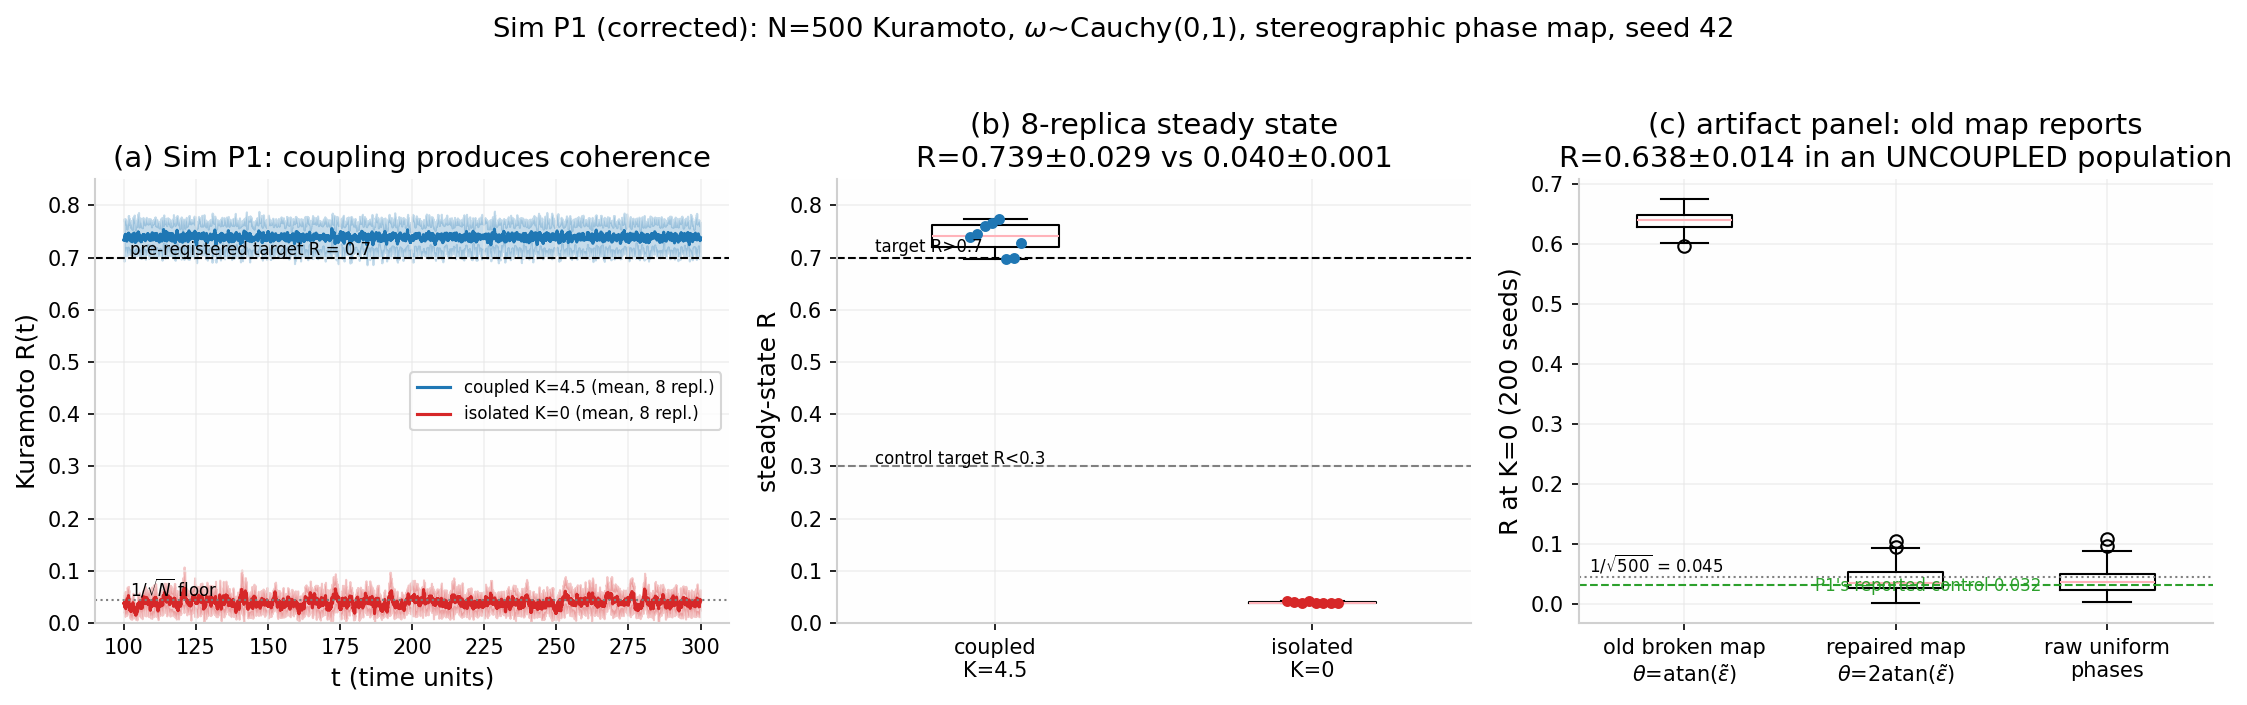
\includegraphics[width=0.92\textwidth]{figures/figP1_coherence.png}
\caption{Sim P1 (\S3.6): the Kuramoto order parameter $R(t)$ under protocol coupling ($K = 4.5$) versus the isolated control ($K = 0$) across 8 replicas, with steady-state distributions (coupled $R = 0.739 \pm 0.029$; isolated $R = 0.040 \pm 0.001$, at the $1/\sqrt{N} \approx 0.045$ finite-size floor) and the phase-map-control side panel: the half-circle $\mathrm{atan}$ initialization reports $R = 0.638 \pm 0.014$ at $K = 0$ (200 seeds), while the corrected stereographic map ($0.040 \pm 0.020$) and raw uniform phases ($0.039 \pm 0.020$) sit at the floor. Verification re-run, seed 42.}
\label{fig:p1}
\end{figure*}

\begin{figure*}[!tp]
\centering
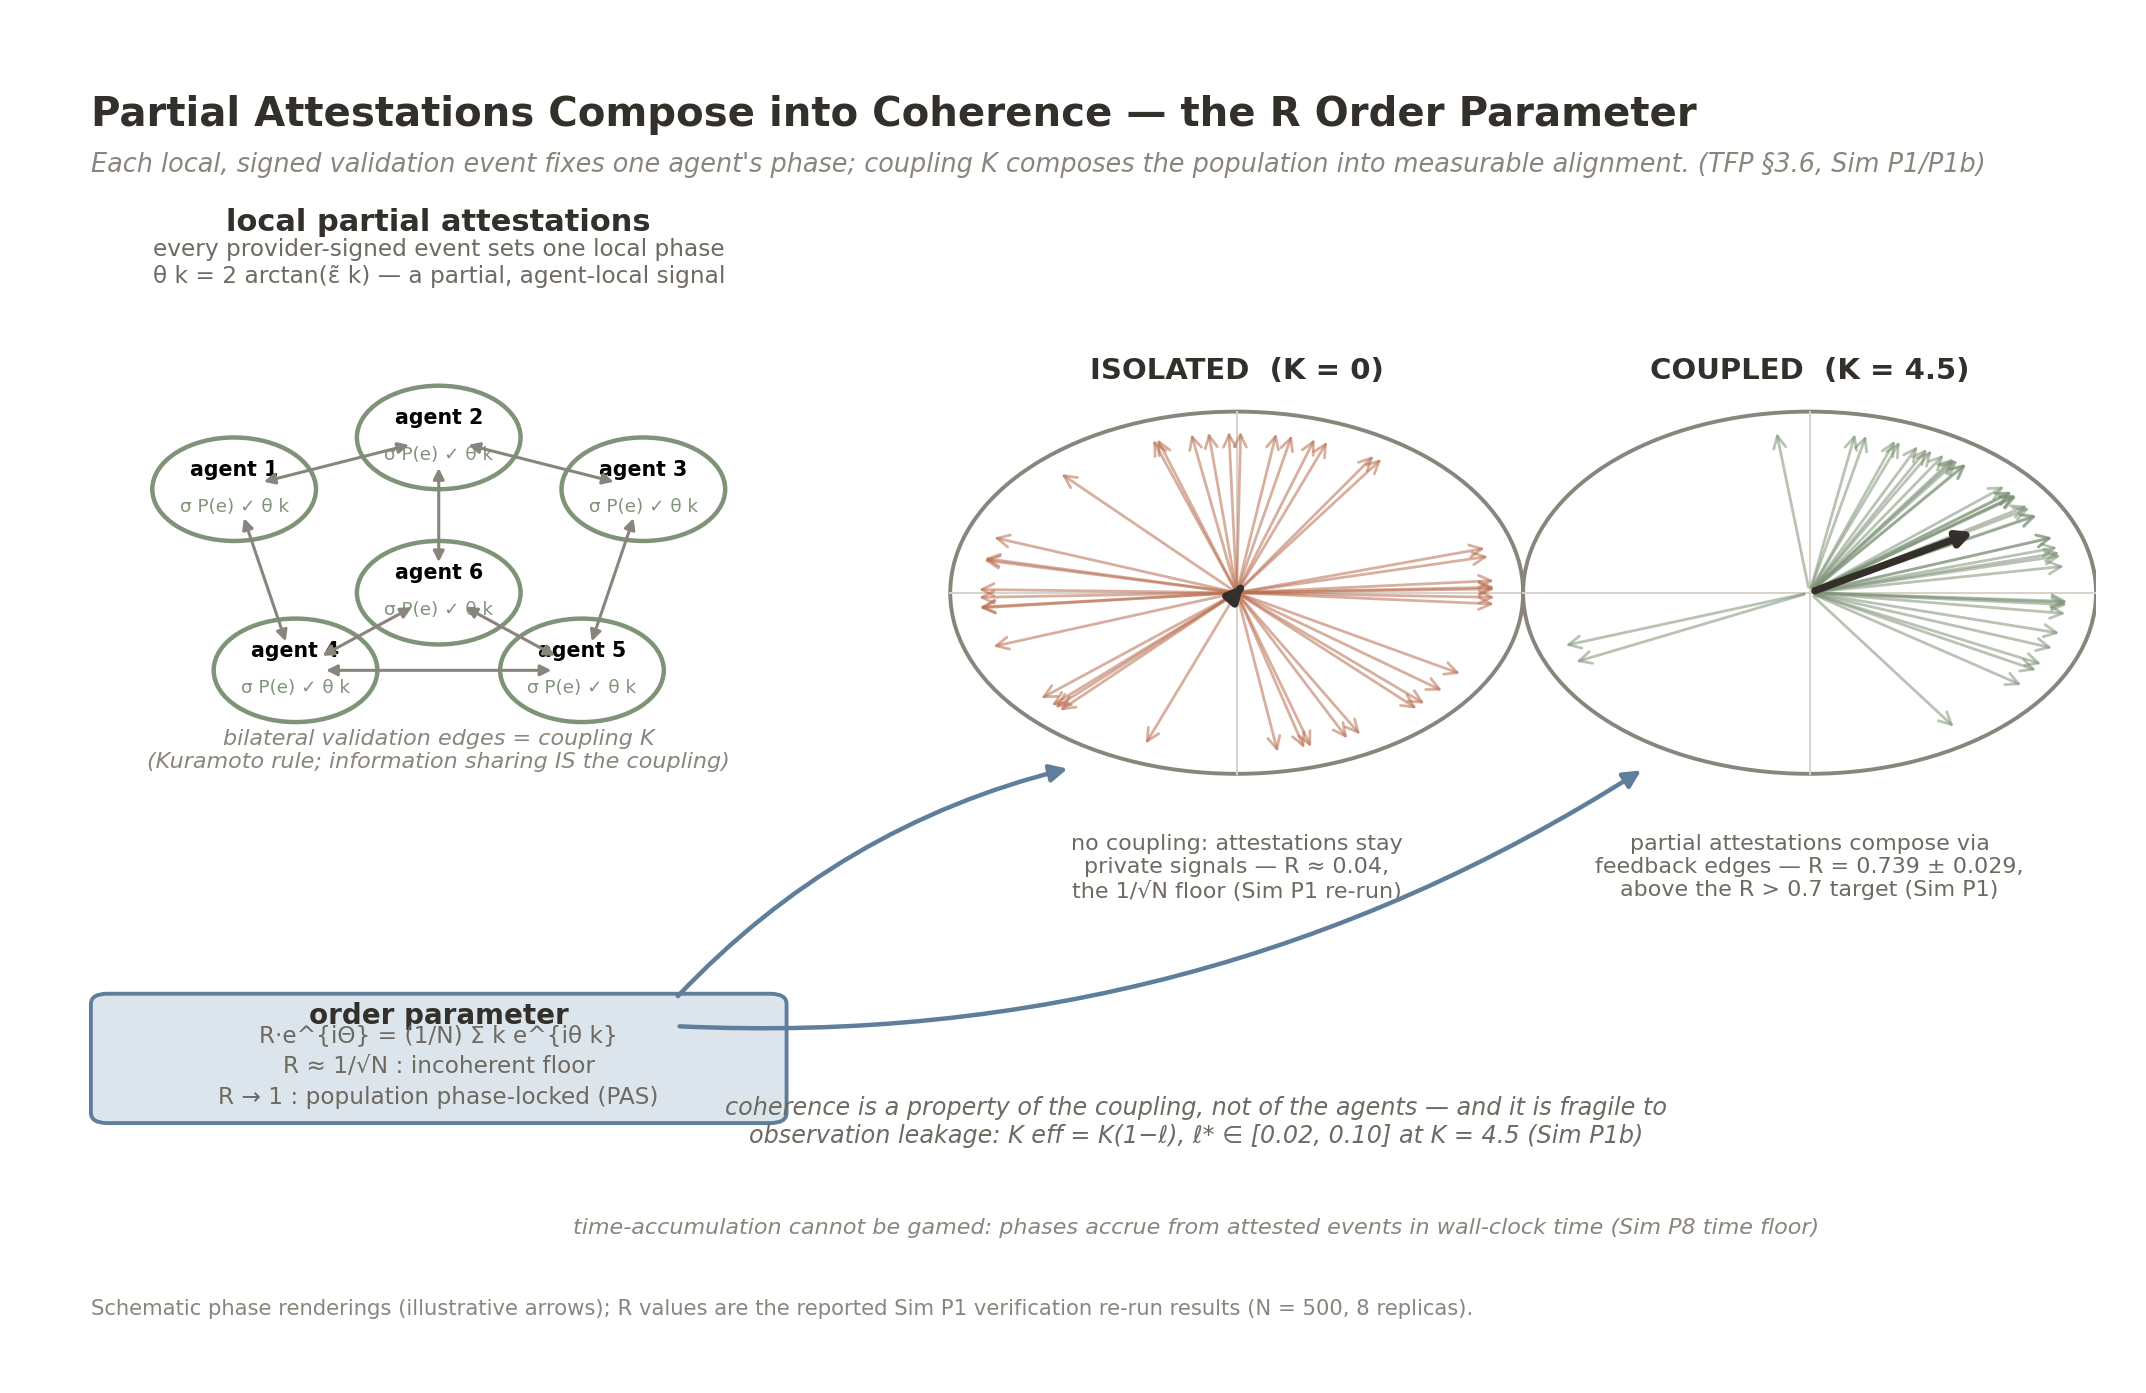
\includegraphics[width=0.92\textwidth]{figures/tfp_pas_coherence.png}
\caption{Partial attestations compose into coherence (\S3.6, Sim P1; schematic). Each provider-signed event fixes one agent-local phase $\theta_k = 2\arctan(\tilde{\varepsilon}_k)$; bilateral validation edges are the Kuramoto coupling $K$; the order parameter $R \cdot e^{i\Theta} = (1/N)\sum_k e^{i\theta_k}$ measures population alignment. Schematic phase renderings: isolated agents ($K = 0$) sit at the $1/\sqrt{N}$ incoherent floor ($R \approx 0.04$); the coupled population ($K = 4.5$) phase-locks ($R = 0.739 \pm 0.029$, Sim P1 verification re-run). Coherence is a property of the coupling, not of the agents, and is fragile to leakage ($K_{\mathrm{eff}} = K(1-\ell)$; the $\ell^{*}$ band at the operating point, Sim P1b); phases accrue from attested events in wall-clock time (the Sim P8 time floor), so accumulation cannot be compressed except by parallel-provider collusion (\S3.7 caveat). Phase arrows are seeded schematic draws; only the printed re-run values are measured.}
\label{fig:pas}
\end{figure*}

\begin{figure*}[!tp]
\centering
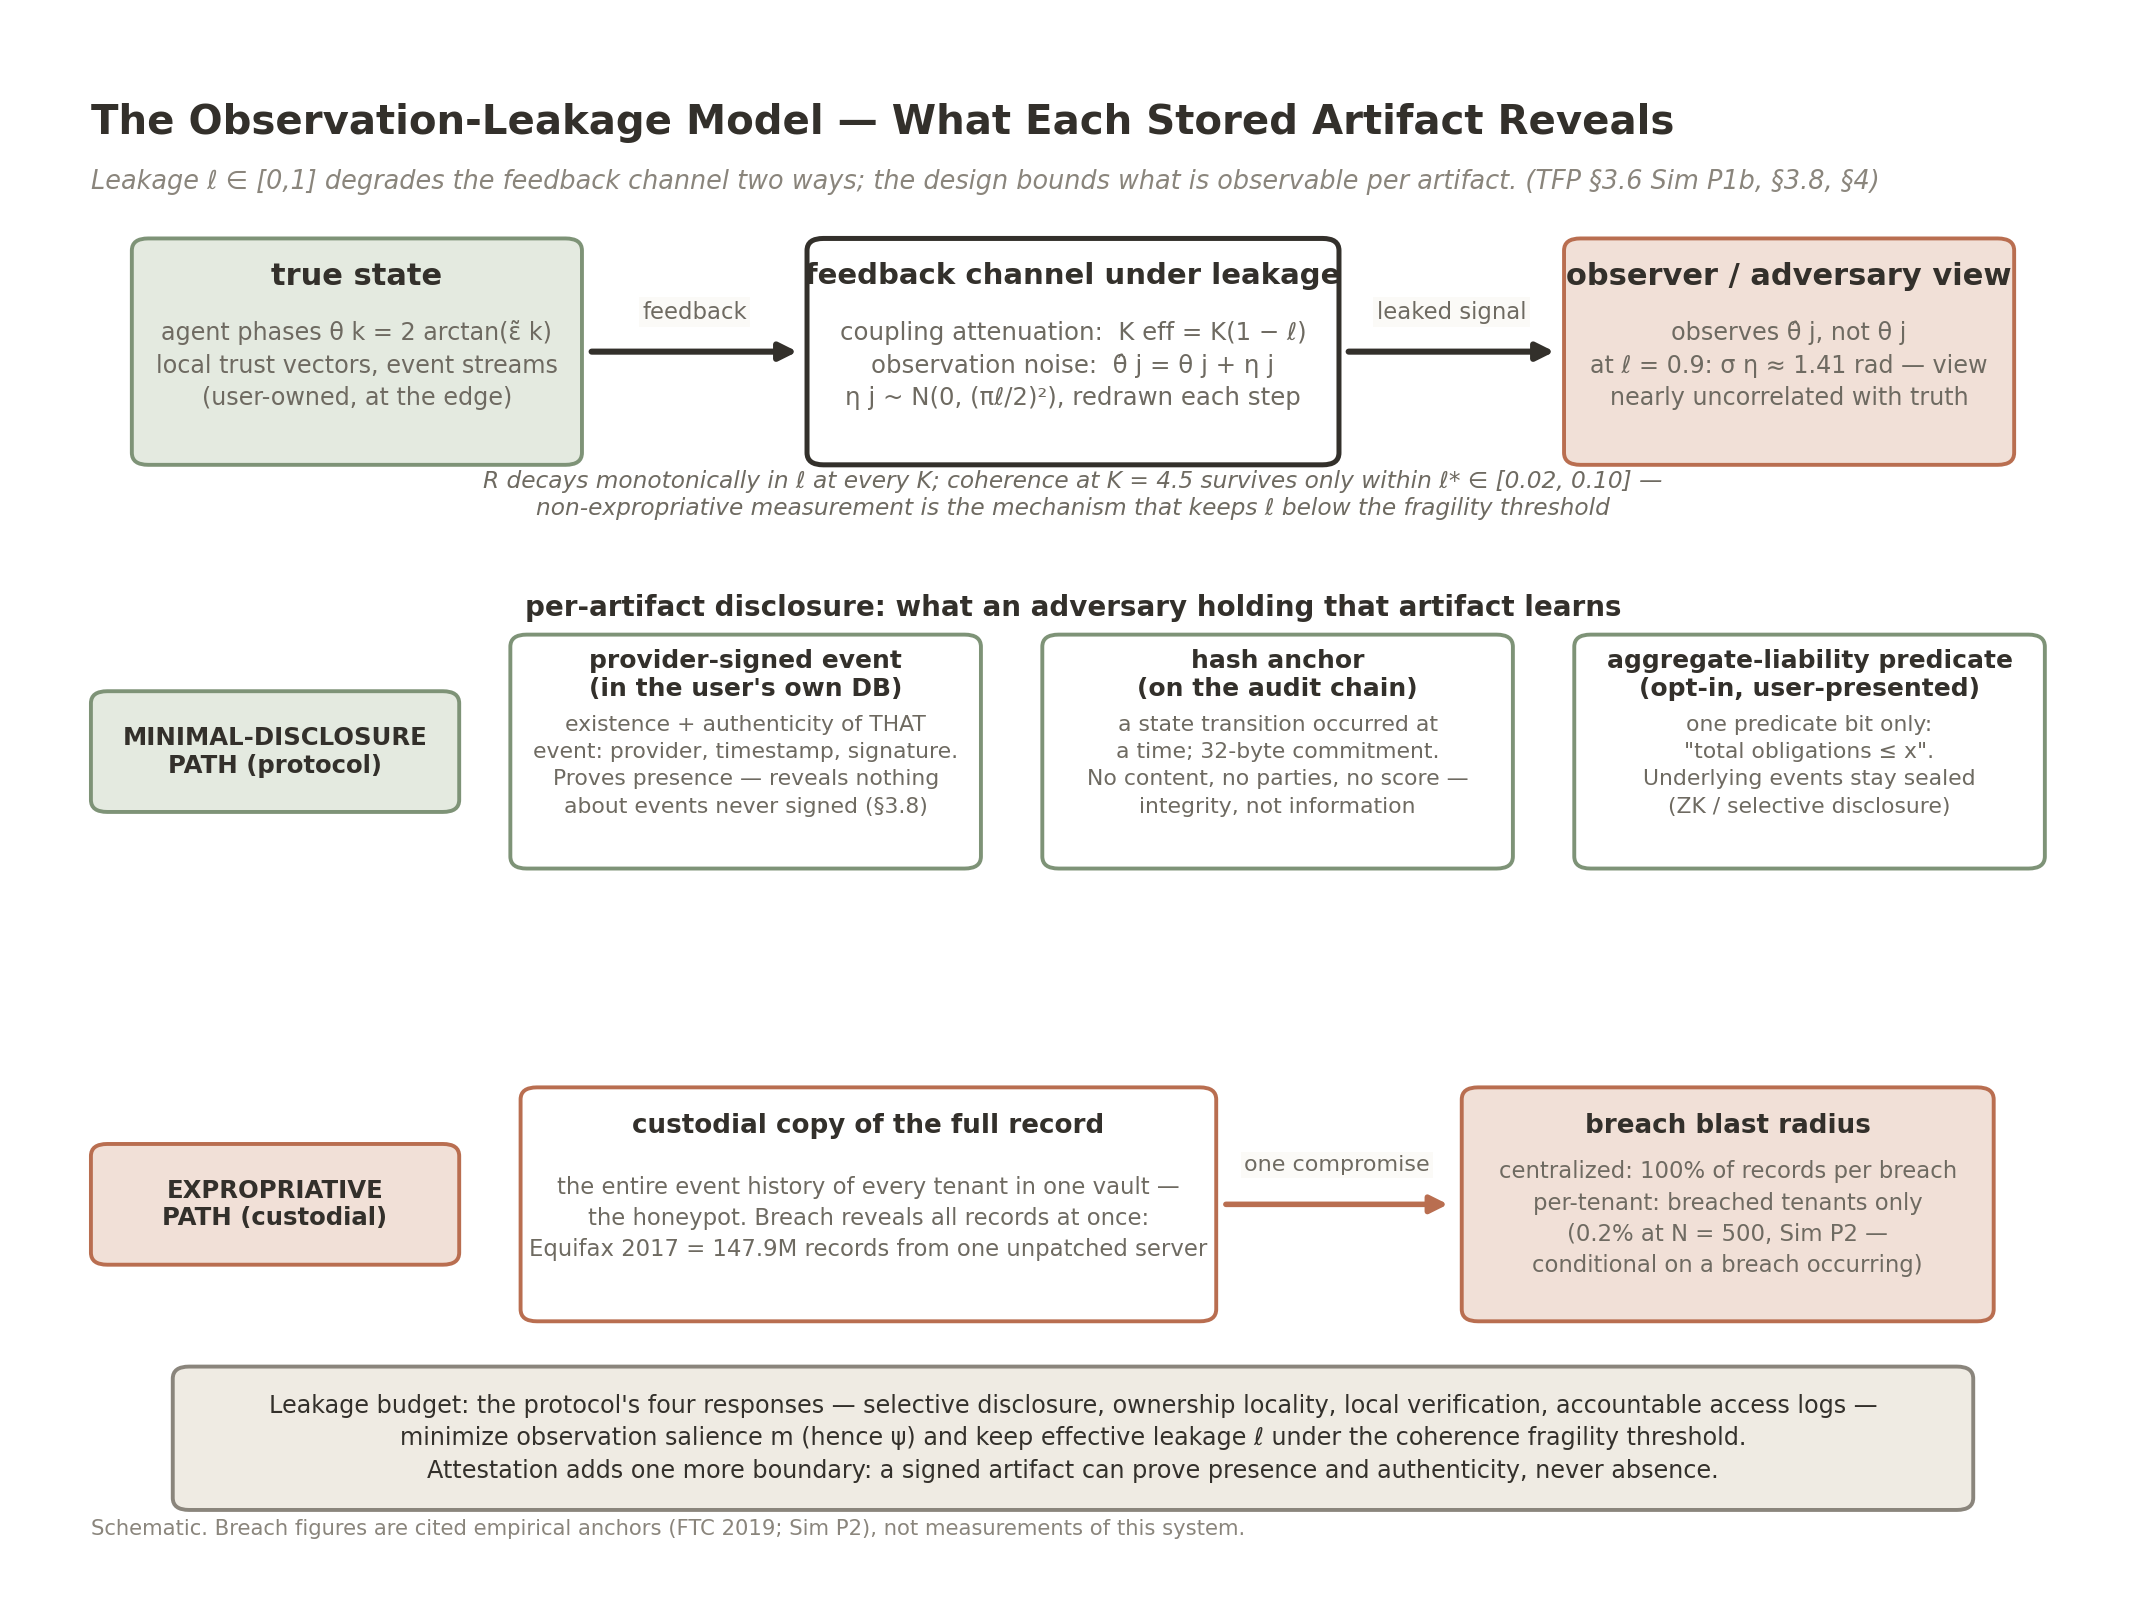
\includegraphics[width=0.92\textwidth]{figures/tfp_leakage_model.png}
\caption{The observation-leakage model (\S3.6, Sim P1b; supports \S3.8--3.9). Top: leakage $\ell \in [0,1]$ degrades the feedback channel two compounding ways --- coupling attenuation $K_{\mathrm{eff}} = K(1-\ell)$ and observation noise $\hat{\theta}_j = \theta_j + \eta_j$, $\eta_j \sim \mathcal{N}(0,(\pi\ell/2)^2)$ --- so the adversary's view decorrelates from the true state as $\ell$ rises (at $\ell = 0.9$, $\sigma_\eta \approx 1.41$ rad). Middle: what each stored artifact reveals --- a provider-signed event reveals that event's existence and authenticity only; a hash anchor reveals that a transition occurred, never content; an opt-in aggregate-liability predicate reveals one predicate bit (minimal-disclosure path) --- versus the custodial path, where one compromise of the full-record vault exposes 100\% of records (Equifax 2017 anchor; per-tenant conditional exposure 0.2\% at $N = 500$, Sim P2). Bottom: the leakage budget, model-internal: $\ell$ has no field operationalization, and the mapping from the four responses (\S4) (or from $m$/$\psi$) to $\ell$ is an unmeasured assumption; in the model, $R > 0.7$ at $K = 4.5$ requires $\ell \lesssim 0.02$--$0.10$.}
\label{fig:leak}
\end{figure*}

\begin{figure*}[!tp]
\centering
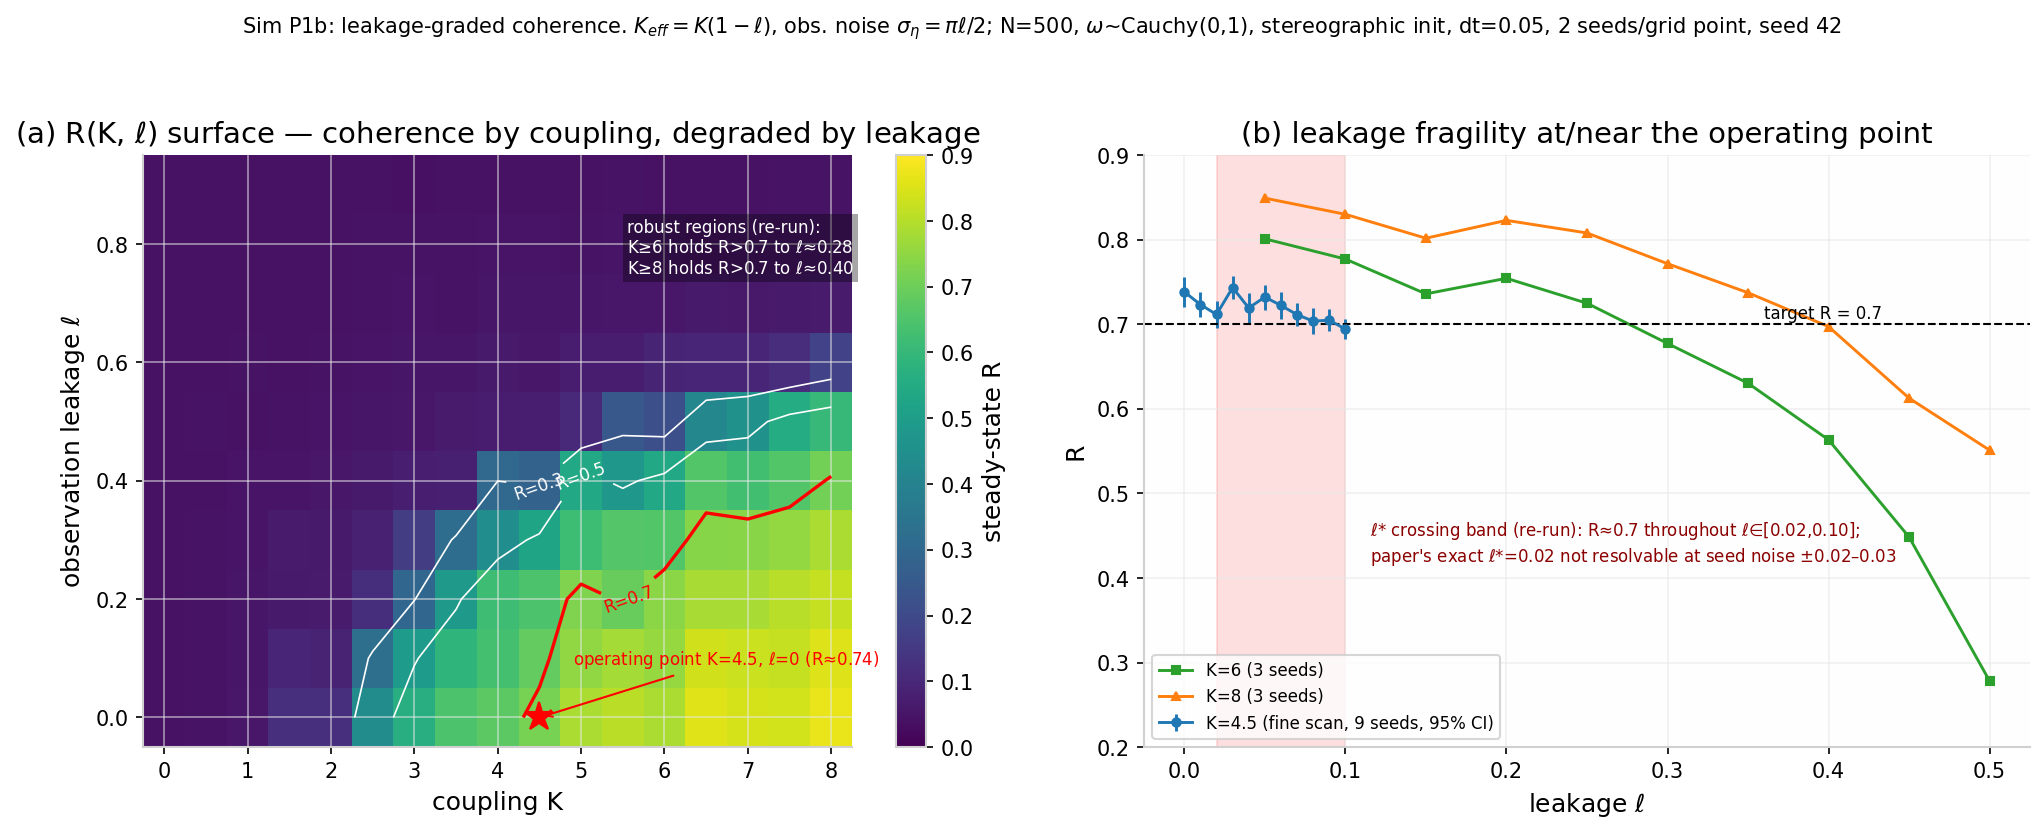
\includegraphics[width=0.92\textwidth]{figures/figP1b_surface.png}
\caption{Sim P1b (\S3.6): the coherence surface $R(K, \ell)$ over $K \in [0,8] \times \ell \in [0,0.9]$ with $R = 0.3/0.5/0.7$ contours and the $K = 4.5$ operating point marked, and the leakage-fragility slice with the crossing band $\ell^* \in [0.02, 0.10]$ (9-seed fine scan). Leakage model: $K_{\mathrm{eff}} = K(1-\ell)$ plus observation noise $\sigma_\eta = \pi\ell/2$ redrawn every timestep; $N = 500$, $\omega \sim \mathrm{Cauchy}(0,1)$, stereographic initialization, $dt = 0.05$. Robust regions (two independent seeded re-renders; point precision not resolvable at these N): $K = 6$ holds $R > 0.7$ to $\ell \approx 0.22\text{--}0.28$; $K = 8$ to $\ell \approx 0.30\text{--}0.40$; the $R = 0.7$ contour sits at $K \approx 5.0\text{--}5.5$ ($\ell = 0.1$) and $K \approx 5.9\text{--}7$ ($\ell = 0.2$), retreating off-grid ($K > 8$) only for $\ell \gtrsim 0.25\text{--}0.4$ across re-renders; $\ell$ is a model-internal parameter with no field operationalization yet.}
\label{fig:p1b}
\end{figure*}



\begin{itemize}
\tightlist
\item
  \textbf{Sim P1 --- Coupling produces PAS coherence {[}SUPPORTED{]}.}
  Under protocol coupling (\(K = 4.5,\) the companion theory preprint's Sim G1 PAS operating
  point), the population synchronizes: \(R = 0.739\) \(\pm\) 0.029
  across 8 replicas (verification re-run, consistent with the first run's 0.751
  (\(\pm\) 0.041) within \(\pm 1\sigma\)), against the
  pre-registered target \(R > 0.7.\) The isolated control (\(K = 0\))
  remains incoherent: \(R = 0.040\) \(\pm\) 0.001 in the re-run (0.032
  in the first run; both sit at the \(1/\sqrt{N}\) \(\approx\) 0.045 finite-size
  floor, whose draws barely vary across replicas; target \(R < 0.3\);
  raw uniform phases). Coherence is a property of the coupling --- the
  composition --- not of the agents, and specifically not of isolation.
  Figure \ref{fig:p1} renders the battery: the order-parameter
  trajectories R(t) of the coupled and isolated arms across the 8
  replicas, their steady-state distributions, and the phase-map-control side panel introduced above (200-seed ensemble).
  Figure \ref{fig:pas} schematizes the mechanism: partial attestations
  fix agent-local phases, validation edges are the coupling, and the
  measured coherence is a property of that composition.
\item
  \textbf{Sim P1b --- Observation leakage degrades coherence
  {[}SUPPORTED qualitatively; HONEST NULL on the quantitative
  threshold{]}.} The leakage-graded arm --- obligation (2) of §1.4 --- maps R over K \(\in\) {[}0, 8{]} \(\times\)
  \(\ell\) \(\in\) {[}0, 0.9{]} (\(N = 500\);
  \(\omega \sim \mathrm{Cauchy}(0,1)\); stereographic initialization; 2
  seeds averaged per grid point; 9-seed fine scan at the operating
  point; 3-seed mid scans at \(K = 6,\) 8). \textbf{Leakage
  operationalization (exact):} the observation-leakage parameter
  \(\ell\) \(\in\) {[}0,1{]} degrades the feedback channel in two
  compounding ways --- (i) \emph{coupling attenuation},
  \(K_{\mathrm{eff}} = K(1 - \ell)\): a fraction \(\ell\) of the
  feedback signal never reaches the population; and (ii)
  \emph{observation noise}, each agent's phase as observed by the others
  is \(\hat{\theta}_j = \theta_j + \eta_j\) with
  \(\eta_j \sim N(0, (\pi\ell/2)^2)\), redrawn independently every
  timestep (at \(\ell = 0.9\), \(\sigma_\eta \approx 1.41\) rad --- the
  observed phase is nearly uncorrelated with the true phase). This is
  the strongest reasonable leakage model, so the reported thresholds are
  conservative. \(\ell\) is a model-internal parameter with no field
  operationalization yet. Figure \ref{fig:leak} schematizes the model and the
  per-artifact leakage budget it implies. \textbf{Results (Figure
  \ref{fig:p1b}).} (a) The R(K,
  \(\ell\)) surface rises smoothly from the \(1/\sqrt{N}\) floor at K
  \(\lesssim 2\) (consistent with the mean-field reference value
  \(K_c = 2/(\pi g(0)) = 2\) for Cauchy\((0,1)\), stated with its
  all-to-all, \(N \to \infty\) assumptions --- a reference, not a
  prediction) to R \(\approx\) 0.85 at \(K = 8,\) \(\ell = 0\); leakage
  compresses the entire surface, and the \(R = 0.7\) contour retreats
  from K \(\approx\) 4.4 (\(\ell = 0\)) to K \(\approx\)
  5.0--5.5 (\(\ell = 0.1\)) and K \(\approx\) 5.9--7
  (\(\ell = 0.2\)), moving off-grid
  (\(K > 8\)) only for \(\ell\) \(\gtrsim 0.25\)--0.4 across re-renders (ranges span two
  independent seeded re-renders; point precision is not resolvable at
  these N). (b) \textbf{Mechanism demonstrated in silico under a stated
  operationalization whose attenuation component is definitional:} R decays monotonically with \(\ell\) at every fixed K ---
  at the operating point \(K = 4.5,\) \(R = 0.709\) (\(\ell = 0\))
  \(\to\) 0.663 (\(\ell = 0.1\)) \(\to\) 0.474 (\(\ell = 0.3\)) \(\to\)
  0.071 (\(\ell = 0.5\)) \(\to\) 0.041 (\(\ell = 0.9,\) at the
  incoherent floor). (c) \textbf{Honest null:} at \(K = 4.5\) the
  zero-leakage coherence is only R \(\approx\) 0.71, \emph{marginally}
  above target, and R falls below 0.7 within the leakage band
  \textbf{\(\ell\)* \(\in\) {[}0.02, 0.10{]}} --- in the 9-seed fine
  scan R hovers at 0.69--0.74 across \(\ell\) \(\in\) {[}0, 0.10{]},
  with the first below-0.7 reading at \(\ell = 0.08,\) so the crossing
  is resolvable only as a band at seed noise \(\pm 0.02–0.03\); the
  a point estimate of \(\ell\)* \(\approx\) 0.02 (with its
  suspiciously smooth 0.705/0.701/0.698 sequence) is not resolvable. R
  falls below 0.5 near \(\ell\) \(\approx\) 0.3 and below 0.1 near
  \(\ell\) \(\approx\) 0.5. The defensible architectural claim is
  therefore: \textbf{non-expropriative measurement (§4's four responses)
  is what keeps \(\ell\) below the fragility threshold} --- and at the
  current operating point that threshold is the band \(\ell\)* \(\in\)
  {[}0.02, 0.10{]}, a demanding requirement, not a soft one. Robust
  \(R > 0.7\) requires K \(= 6\) (coherence survives to \(\ell\) \(\approx\) 0.22--0.28) or K \(= 8\)
  (to \(\ell\) \(\approx\) 0.30--0.40), or a lower
  coherence target. The qualitative mechanism --- leakage erodes
  coherence --- is robust; the quantitative threshold at \(K = 4.5\) is
  fragile, and this paper says so. \textbf{Definitional component:} component (i) of the leakage operationalization
  (\(K_{\mathrm{eff}} = K(1-\ell)\)) makes part of the R-decay
  definitional --- Kuramoto coherence decreases monotonically in
  coupling by construction; the non-definitional content is component
  (ii) (observation noise) and the joint surface's quantitative
  thresholds. The identification of expropriative observation with
  channel attenuation is a modeling assumption, not a derivation; the
  \(\psi\)-model (companion theory preprint, \S3.3) is the stack's mechanistic account of
  chilling.
\item
  \textbf{Sim P1c --- Sparse/weighted-network sensitivity {[}the
  functional form SURVIVES; the \(K = 4.5\) operating point FAILS
  under sparsity{]}.} A further battery (SIM-R2 battery 4, seed 42;
  code and curves bundled with the Supporting Document (deposit pending)) re-runs the
  Sim P1 protocol exactly --- \(N = 500\), \(\omega \sim
  \mathrm{Cauchy}(0,1)\), stereographic initialization, Euler
  \(dt = 0.05\), burn-in 100 t.u.\ + measurement 200 t.u., 2 graph
  realizations \(\times\) 2 seeds per topology --- with the coupling
  degree-normalized (\(K/k_i\), a disclosed choice that keeps \(K\)
  comparable across topologies and isolates the uncoupled) on
  Erd\H{o}s--R\'enyi (\(p \in \{0.05, 0.1, 0.2, 0.5\}\),
  \(\langle k\rangle \approx 25/49/100/249\)), Barab\'asi--Albert
  (\(m = 12\) and \(m = 2\), \(\langle k\rangle \approx 24\)
  and 4), and all-to-all with symmetric log-normal\((0, 0.5)\) weights
  rescaled to mean 1. Validation: the all-to-all arm reproduces the
  published operating point (\(R(K = 4.5) = 0.710 \pm 0.029\) vs.\ 
  0.709); the Sim P1 verification re-run's \(0.739 \pm 0.029\) at
  the same nominal operating point differs because P1's
  ABM-with-adversaries protocol and P1c's pure-Kuramoto protocol
  differ --- the \(\sim\)0.03 gap is within seed noise. Results: \textbf{\(R > 0.7\) at \(K = 4.5\) does not
  survive sparsity} --- ER \(p = 0.05 \to 0.684 \pm 0.036\); BA
  \(m = 12 \to 0.687 \pm 0.024\) (both below target, within
  \(\sim\)1 sd); BA \(m = 2 \to 0.416 \pm 0.061\), collapsing and
  never recovering above 0.7 even at \(K = 8\) (0.660) --- while ER
  \(p \geq 0.2\) (0.705--0.709) and the log-normal-weighted
  all-to-all (0.710) pass. \textbf{The threat is missing edges (mean
  degree \(\langle k\rangle \lesssim 25\)), not heterogeneous
  weights.} The functional form is robust where the level is not:
  every topology shows the same continuous onset at \(K_c \approx 2\)
  (the mean-field \(K_c = 2\) for Cauchy\((0,1)\) survives under
  degree normalization); what shifts is the asymptote level and the
  margin above threshold. Product reading, stated against Sim P1b's
  own fragility band: the already-thin \(\ell\)-band at \(K = 4.5\)
  (\(\ell^{*} \lesssim 0.02\)--0.10) is further compressed on
  sparse networks --- a real trust network with effective degree
  \(\sim\)25 sits \emph{below} the \(R = 0.7\) line even at zero
  leakage --- so the defensible claim needs \(K \geq 6\)--8 \emph{and}
  \(\langle k\rangle \gtrsim 25\) (Figure~\ref{fig:p1c}).

  \begin{figure}[!tb]
  \centering
  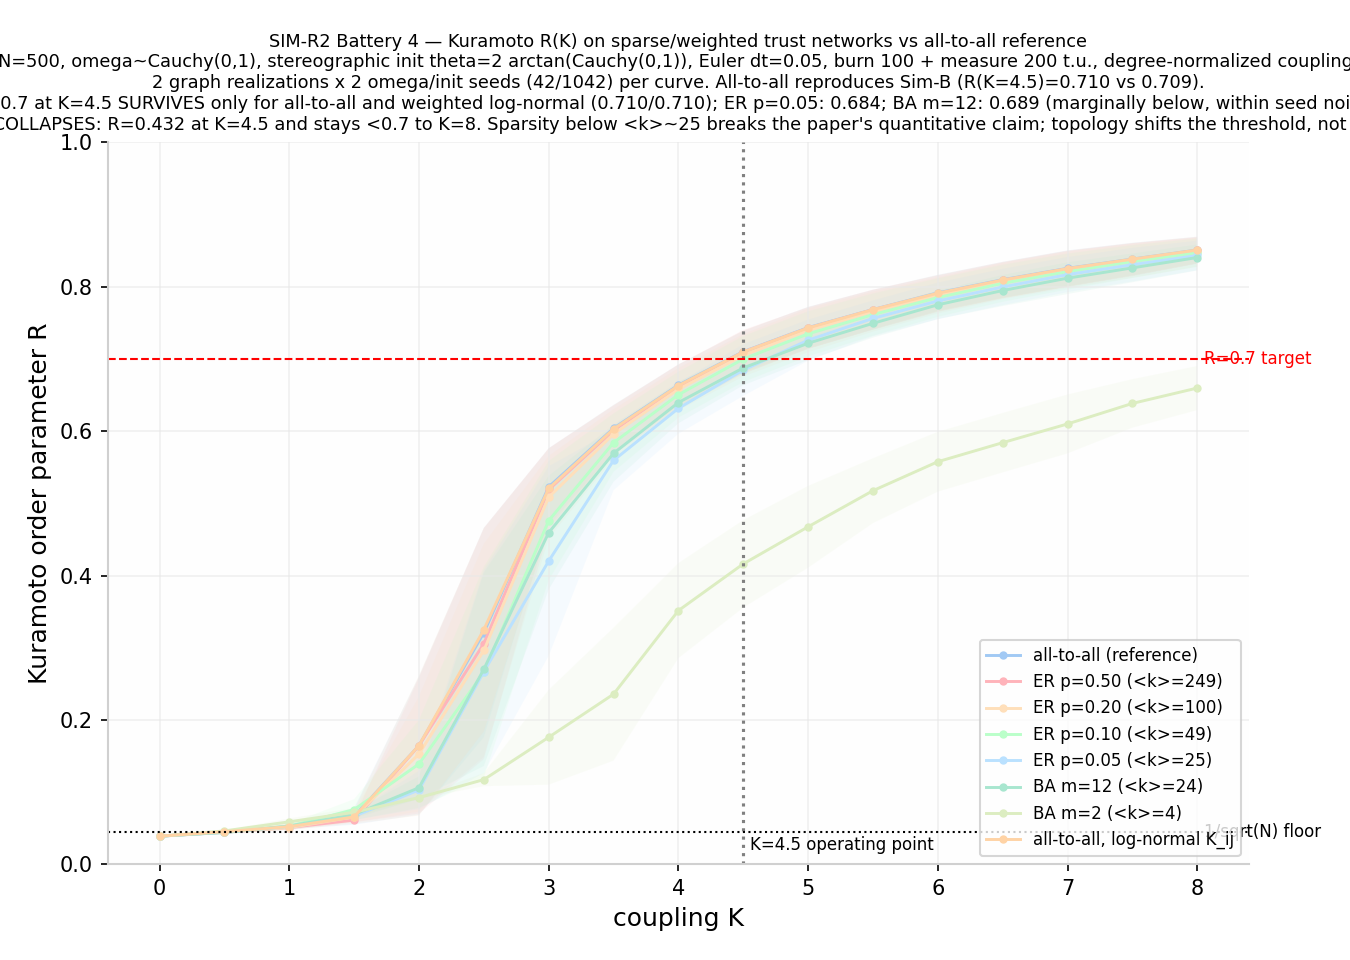
\includegraphics[width=\columnwidth]{figures/figR2_B4_kuramoto_topologies.png}
  \caption{Sim P1c (\S3.6): sparse/weighted-network sensitivity of the Kuramoto coherence claim (SIM-R2 battery 4, seed 42). $R(K)$ per topology (mean $\pm$ sd over 2 graph realizations $\times$ 2 seeds) against the all-to-all reference, with the $R = 0.7$ target, the $1/\sqrt{N}$ floor, and the $K = 4.5$ operating point marked. The continuous onset at $K_c \approx 2$ is topology-invariant; the $K = 4.5$ coherence level fails for $\langle k\rangle \lesssim 25$ (ER $p = 0.05$: 0.684; BA $m = 12$: 0.687; BA $m = 2$: 0.416) and survives weight heterogeneity (log-normal weighted all-to-all: 0.710).}
  \label{fig:p1c}
  \end{figure}
\item
  \textbf{Sim P2 --- Attack-surface reduction, conditional on breach
  {[}SUPPORTED{]}.} Monte-Carlo breach comparison (1,000
  epochs): \emph{given that a breach occurs}, a breach of the
  centralized shared record compromises 100\% of records; a breach under
  database-per-tenant isolation compromises exactly the breached tenants
  (0.2\% at \(N = 500\)) --- a 99.8\% relative reduction \emph{in
  conditional exposure}, against the pre-registered \(\geq 98%
  \) target. \textbf{This is a statement about blast radius given a
  breach, not about risk.} The probability side of the risk equation ---
  distribution multiplies attackable endpoints from a handful of
  custodians to millions of user devices --- is modeled in §3.9, where
  the headline is variance reduction, not loss elimination.
\item
  \textbf{Sim P3 --- Marginal-cost scaling form {[}SUPPORTED for the
  scaling form; the static reduction claim is restated{]}.} Per-event
  settlement at x402-class sub-cent cost is per-tenant with no shared
  queue: marginal cost per additional user is constant (\$0.001/event)
  from N = \(10^{3}\) to \(10^{6}\). Two disciplines govern the
  comparison. \textbf{(i) Like-for-like only.} A ``\$50 per record pull''
  anchor --- a full-service product price (lender-paid, inclusive of labor,
  liability, and compliance) from the financial deployment, documented in the
  financial application preprint (specified separately) --- is not commensurate with the
  protocol's \emph{marginal} settlement fee, and no headline reduction derived
  from it (e.g., ``99.998\% below baseline'') is claimed. The defensible
  comparison is marginal-vs-marginal: x402-class settlement at
  \$0.001/event against the incumbent's marginal per-query cost (metered
  per-request API pricing; incumbent per-query prices are
  vendor-specific and unpublished, so the reduction factor is maintained
  against the versioned calculator rather than printed). On equal
  event/query counts n, the protocol exceeds a 98\% marginal-cost
  reduction exactly when the incumbent's marginal per-query cost exceeds
  \$0.05/query --- a conditional statement, not a headline. \textbf{(ii)
  Events-per-decision accounting.} A per-event cost becomes a
  per-decision cost only through an event count. Stated assumption: an
  application-level decision consumes \(10^{3}–10^{5}\) validation
  events (frozen assumption for the print figures; per-application
  values are the financial application preprint's responsibility). At \$0.001/event, that is
  \textbf{\$1--\$100 of settlement per decision}; adding edge compute
  (participant's own device: marginal electricity) and backup storage
  ($\sim$1 GB/tenant-year at \$0.014--0.019/GB, i.e.~cents per
  year) does not move the range. Whether the protocol's per-decision
  cost beats an incumbent's per-decision cost therefore depends on the
  event-count assumption and the incumbent's marginal (not full-product)
  price; the \(>\)98\% target of H1 leg 3 survives only at the
  low end of the events-per-decision range and is restated accordingly.
  Sim P3 thus demonstrates the \emph{scaling form} of the cost claim ---
  constant marginal cost, no shared queue, no queueing collapse at
  \(10^{6}\) users --- and nothing more; §5.2 prints the frozen figures.
\end{itemize}

A follow-on run couples the population model to the measurement layer
(full protocol and statistics in the Supporting Document, §N): each
agent class's trust sensitivity \(\lambda_i\) is seeded from the
category-resolved cortical effect sizes model-predicted by the TRIBE v2
forward-encoding runs on the biological layer (companion biology preprint, §5.2;
\(\lambda_i = \lambda_{\mathrm{base}}(1 + g z_i)\), \(g = 0.5\) frozen
before the run), so the population's heterogeneity is no longer assumed
but inherited from the layer below as simulation seeding parameters ---
model-predicted quantities, not measurements (the companion biology preprint, §5.2, labels them
``not a measured quantity''). Two seedings were run --- one from the
  six-offer measurement, one from the 27-stimulus battery --- and
they are reported together because they differ.

\begin{itemize}
\tightlist
\item
  \textbf{Sim P4a --- Heterogeneous-coupling PAS {[}SUPPORTED, with a
  caveat{]}.} The population synchronizes under model-predicted (battery-derived) heterogeneity:
  \(R = 0.759\) \(\pm\) 0.024 against the pre-registered \(R > 0.7.\)
  Caveat: in the current agent model the phase
  dynamics are decoupled from the trust-vector update, so R is identical
  under any \(\lambda\) seeding --- P4a confirms the population coheres
  at \(K = 4.5\) but does not by itself exercise the heterogeneity. The
  informative test is P4b.
\item
  \textbf{Sim P4b --- Heterogeneity leaves a detectable but practically
  negligible footprint {[}SUPPORTED in the statistical sense only{]}.} With battery-derived
  model-predicted sensitivities (\textsc{trust\_signal} \(0.307 >\) \textsc{control}
  \(0.240 >\) \textsc{threat} \(0.176 >\) \textsc{teaser} \(0.158 >\)
  \textsc{predatory} \(0.111 >\) \textsc{fair} \(0\), z-scored), the
  terminal trust-vector distribution of the heterogeneous population is
  \emph{statistically} distinguishable from the homogeneous reference:
  energy distance 0.00021, permutation \(p = 0.005\) (2,000
  permutations) against the pre-registered \(p < 0.05.\) A lower-powered
  seeding --- single offer per category, chain-rule estimate for
  \textsc{trust\_signal} --- gives \(p = 0.109\) (not significant); the
  null is preserved in the record (Supporting Document §N.5). What the result
  actually shows is narrower than the old headline: the seeding variable
  is \textbf{not inert} --- model-predicted (battery-derived) heterogeneity produces a
  statistically detectable difference in where agents end up --- but an
  energy distance of 0.00021 is \textbf{practically negligible} at the
  tested scale, so ``heterogeneity matters for terminal outcomes'' is
  supported only in the statistical sense, not in the effect-size sense,
  and only under the better-powered seeding.
\end{itemize}

These results establish that the composed architecture exhibits its
claimed population-level properties in silico --- and, in P1b, where
those properties break. They do not substitute for deployment
measurements.

\subsection*{3.7 Network, information, and behavioral-agent results (Sim
P5--P8)
{[}SIMULATION{]}}

The §3.6 population runs establish what the protocol does at the
collective-dynamics level; they do not yet test the properties that
distinguish the architecture from its surveillance alternative at the
network level: who learns from whom, how far a compromise reaches, and
whether the validation stream protects boundedly rational agents. A
fourth simulation battery (seed 20260905; full protocol, estimator
details, and the complete audit trail in the Supporting Document, §Q)
tests exactly these, using the standard instruments of each relevant
literature --- transfer entropy for directed information flow
\citep{schreiber2000}, cascade propagation on custody topologies, and
\(\beta\delta\) present-biased agents for behavioral response
\citep{thaler1981,laibson1997}. All criteria were pre-registered in
code; all reported runs are bit-identical under re-execution.

\begin{figure*}[!tp]
\centering
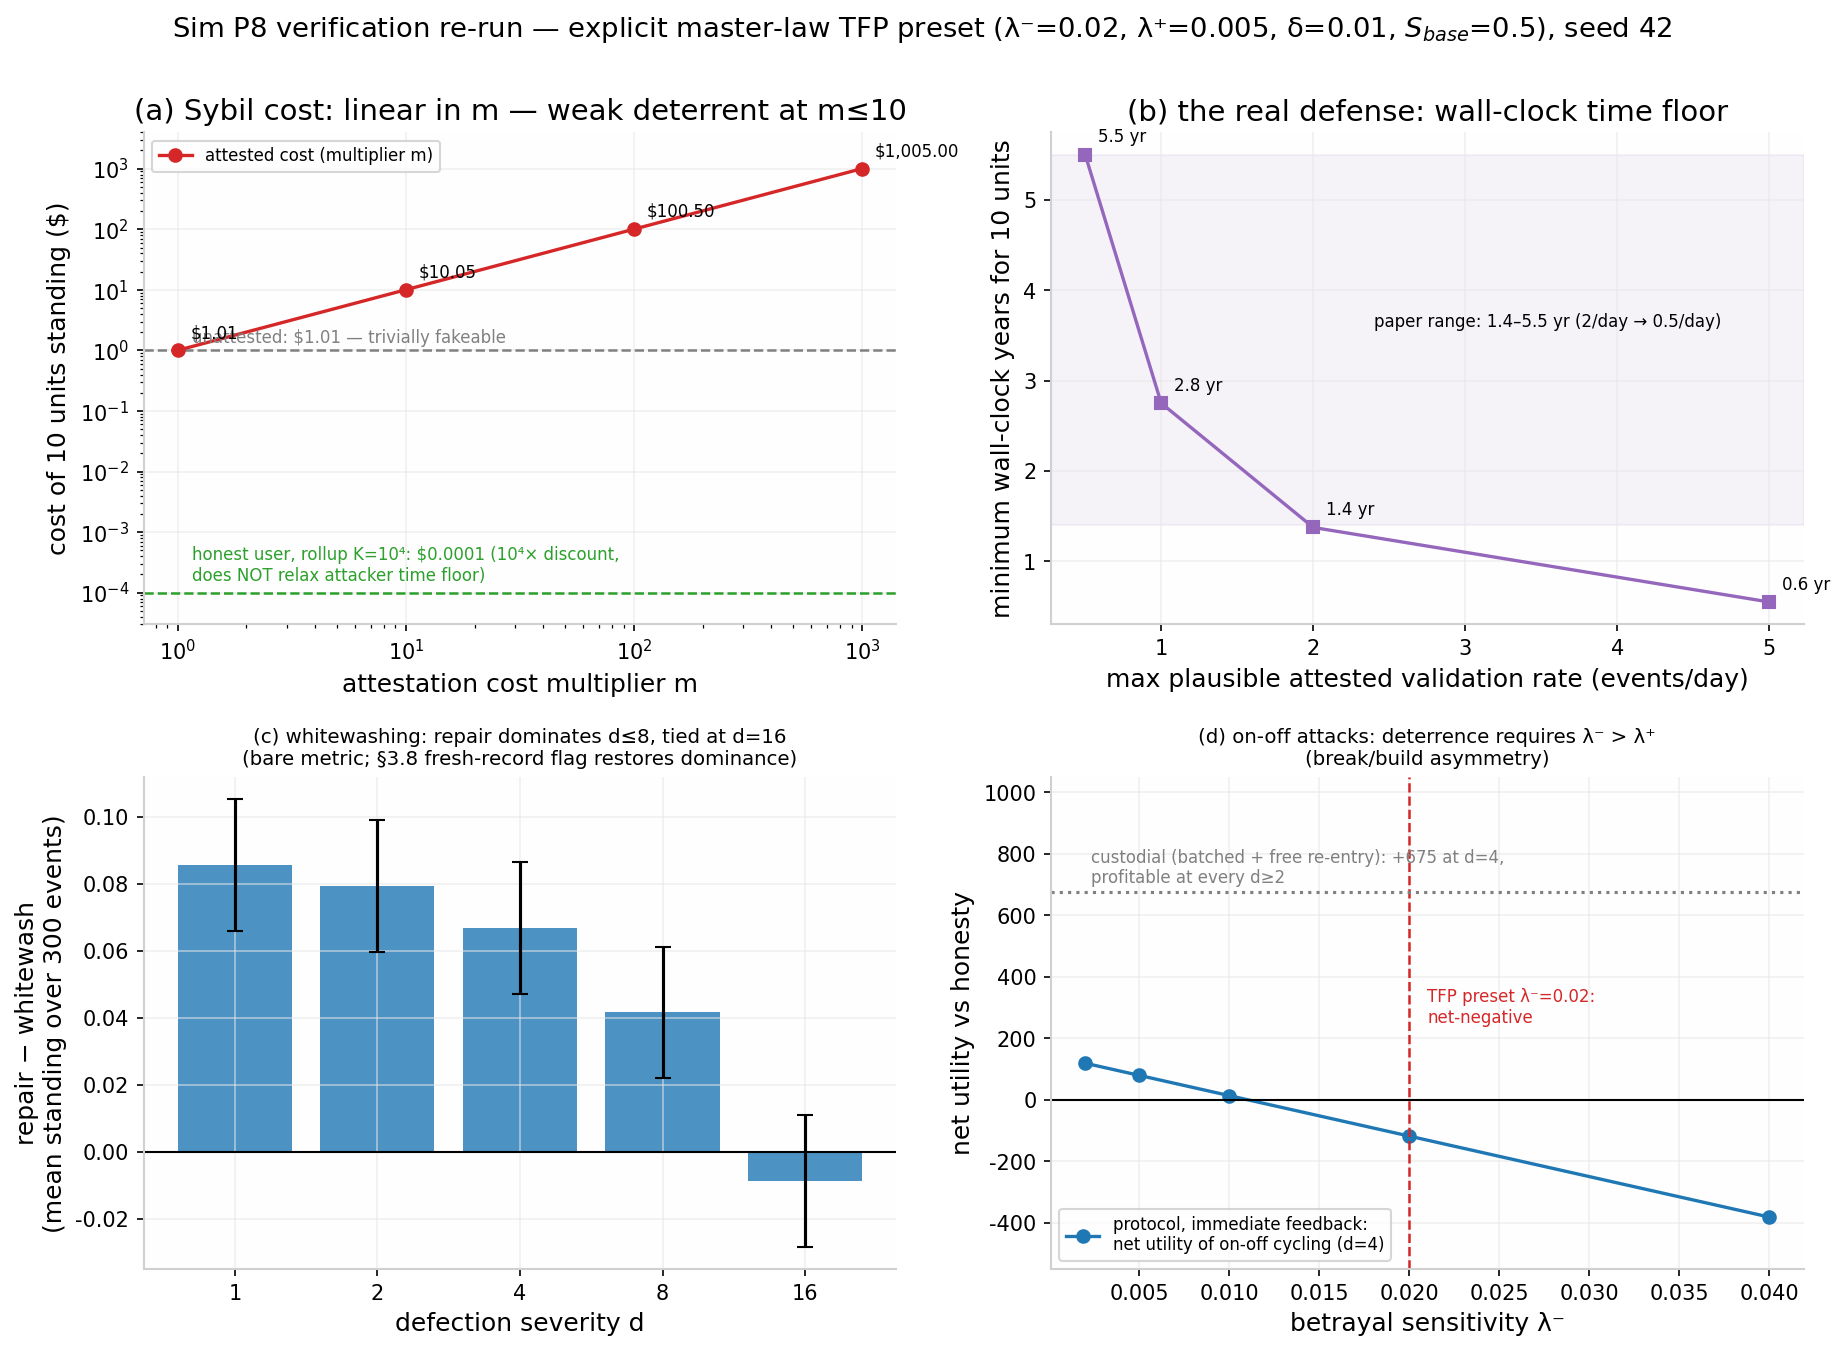
\includegraphics[width=0.92\textwidth]{figures/figP8_sybil_deterrence.png}
\caption{Sim P8 (\S3.7), explicit master-law preset $\lambda^{-} = 0.02$, $\lambda^{+} = 0.005$, $\delta = 0.01$/event: (a) Sybil cost versus attestation multiplier $m$ (log--log; \$1.01 unattested $\to$ \$1{,}005 at $m = 1{,}000$ for 10 units of standing) with the block-rollup honest-cost baseline ($10^{-7}$/event at $K = 10^{4}$ events per anchor); (b) the wall-clock time floor quoted per rate (5.5/1.4 years for 1{,}005 attested events at 0.5/$\leq$2 events/day; $\sim$0.55--1.1 years at the model's own high-standing rates of 2.5--3.76 events/day, 5/day max grid; 0.73 yr at 3.76/day; 0.55 yr at 5/day; parallel-provider collusion divides the floor, \S3.7); (c) repair-versus-whitewash standing advantage by defection severity --- significant for $d \leq 8$, statistically tied at $d = 16$ under the bare standing metric; (d) on-off cycling net utility versus $\lambda^{-}$: net-negative exactly at the $\lambda^{-} = 0.02$ preset under immediate feedback, while custodial batched feedback with free re-entry stays profitable at every $d \geq 2$.}
\label{fig:p8}
\end{figure*}

\begin{figure*}[!tp]
\centering
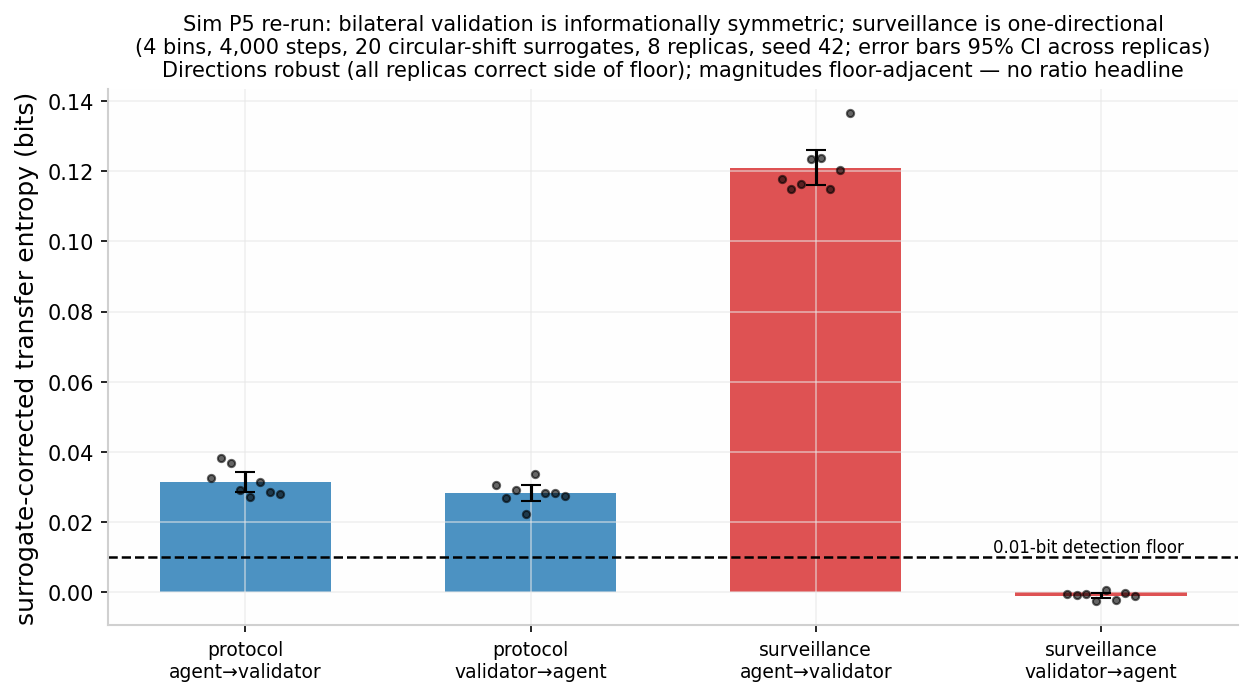
\includegraphics[width=0.92\textwidth]{figures/figP5_transfer_entropy.png}
\caption{Sim P5 (\S3.7): surrogate-corrected transfer entropy between agent and validator under bilateral validation (protocol: $0.0315 \pm 0.003$ / $0.0283 \pm 0.002$ bits) versus surveillance ($0.121 \pm 0.005$ / $-0.001 \pm 0.001$ bits), 95\% CIs across 8 replicas, with the 0.01-bit detection floor marked; every replica lands on the correct side of the floor in both architectures. Magnitudes are floor-adjacent, so no ratio headline is reported.}
\label{fig:p5}
\end{figure*}

\begin{itemize}
\tightlist
\item
  \textbf{Sim P5 --- Information-flow symmetry {[}SUPPORTED, with a
  detection-floor caveat{]}.} Directed information flow between a fixed
  agent and a validator, measured by surrogate-corrected transfer
  entropy (\citealp{schreiber2000}; 4 bins, 4,000 steps, 20
  circular-shift surrogates), is bidirectional under the protocol's
  bilateral-validation architecture (agent\(\to\)validator
  \(0.0315 \pm 0.003\) bits, validator\(\to\)agent \(0.0283 \pm 0.002\)
  bits --- 95\% CIs across 8 replicas; every replica above the 0.01-bit
  detection threshold in both directions) and one-directional under the
  surveillance architecture (agent\(\to\)validator \(0.121 \pm 0.005\)
  bits, validator\(\to\)agent \(-0.001\) \(\pm\) 0.001 bits ---
  surrogate overcorrection to \(\approx\) 0; every replica at or below
  threshold in the return direction). The pre-registered hypothesis ---
  bilateral validation is symmetric, surveillance is not --- survives a
  bias-corrected estimator; the uncorrected estimator inverts the result
(audit trail, §Q.3).
  \textbf{Caveats:} the reported quantities sit within
  roughly \(2.8\times\)--\(12\times\) of the 0.01-bit detection floor, so the
  \emph{directions} of flow are robust (every replica on the correct
  side of the threshold) while the \emph{magnitudes} are floor-adjacent
  estimates; no ratio headline (e.g., ``surveillance extracts roughly four times more   information'') is claimed --- unreliable at these floor-adjacent magnitudes. Per-replica confidence intervals were not computed in the first battery and are registered as a re-run requirement for the Supporting Document.
\item
  \textbf{Sim P6 --- Custody topology and cascade reach {[}structural argument; no cascade model
  claimed{]}.} A DebtRank-style cascade \citep{battiston2012} is not
  applied to data custody, for two reasons.
  \textbf{(i) Category error:} DebtRank models distress propagation
  through interbank \emph{balance-sheet exposure} --- nodes are
  institutions, edges are debt/credit exposures, the state variable is
  equity loss. A breached data custodian leaks entrusted records
  regardless of any counterparty's equity; records are not debts, breach
  exposure does not transmit proportionally through balance sheets, and
  TFP's tenants are not nodes in a lending network. No established
  cascade model for centralized-vs-distributed \emph{data} custody
  exists; we state this as a literature gap rather than borrow a model
  from the wrong substrate (the nearest quantitative precedent is the
  cyber-accumulation literature in insurance, which prices correlated
  loss from shared infrastructure). \textbf{(ii) Tautology risk:} an
  ``isolation stays at \(1.0\times\)'' figure would be true by
  construction --- there are no edges --- a test that could not fail. What is claimed,
  stated for what it is: per-tenant isolation bounds cascade reach
  \emph{by construction} (a compromise cannot propagate along edges that
  do not exist), and connectivity of any kind is the propagation channel
  --- a structural observation, not a measurement. The
  \emph{quantitative} security comparison, with the probability side
  restored, is §3.9's expected-loss analysis; the qualitative
  concentration argument --- shared clients and dependencies re-create
  common-mode failure even under per-tenant custody (\citealp{geer2003},
  software monoculture; §3.9 precedents) --- is the supportable form of the custody-concentration point.
\item
  \textbf{Sim P7 --- Behavioral-agent protection {[}SUPPORTED, with a
  stated sensitivity gap{]}.} A population of present-biased agents
  (\(\beta \sim U(0.4, 0.9)\), \(\delta \sim U(0.95, 0.999)\), horizons
  6--24 steps) is offered adversarial contracts whose deferred cost
  exceeds the agent's \(\beta\)-discounted perception. With the
  immediate-validation stream ON --- which renders the deferred cost
  salient, partially correcting effective present bias --- uptake falls
  from 0.725 to 0.284, a mean paired reduction of 0.441, permutation
  \(p = 0.004\) (2,000 sign-flips, 8 replicas). This is the agent-level
  mechanism behind §4's observation-distortion argument run in the
  protective direction: the same immediacy that surveillance weaponizes
  is what lets validation inform the agent in time to matter.
  \textbf{Limitation (added):} the protective effect runs through a
  salience parameter --- how strongly the validation stream raises the
  subjective weight of deferred cost --- and that parameter was
  \emph{not} swept in the original battery; the size of the uptake
  reduction should be read as existence-of-effect at one salience
  setting, not as an effect-size estimate. A salience-parameter
  sensitivity analysis is registered as a Supporting Document re-run;
  its absence is a stated limitation, and it interacts with §4's finding
  that the protocol's own measurement salience is minimized but nonzero.
\item
  \textbf{Sim P5b --- Heavy-tailed event outcomes (stylized-fact check)
  {[}SUPPORTED{]}.} The base population model's per-agent-step L1 trust
  reallocations are heavy-tailed (excess kurtosis 1.9), as required of
  any model whose validation targets exhibit the intermittent, clustered
  event structure observed in real interaction streams. This follows the
  complexity-economics validation norm --- agent-based models are
  validated against stylized facts and emergent macro-patterns, not
  point forecasts \citep{arthur1999,beinhocker2006,farmer2009}.
\item
  \textbf{Sim P8 --- Canonical attack strategies, and the honest cost of
  manufactured history {[}SUPPORTED{]}.}
  A fifth battery (seed 20260907; protocol and criteria in the
  Supporting Document, §R) instantiates the reputation-systems attack
  taxonomy \citep{hoffman2009,jalaly2023} --- the computational
  continuation of the iterated-trust-game lineage from the Axelrod
  tournaments through its canonical public demonstration
  \citep{case2017} --- against the protocol's update rule, against a
  custodial-reputation baseline (free identity creation at default
  standing, no history-depth term, batched feedback). Figure \ref{fig:p8}
  renders the battery. Update-law provenance, stated per the Technical
  Appendix's mathematical development (§M): the protocol layer of the
  master law is the asymmetric preset \(\lambda^{-} > \lambda^{+}\)
  (break/build asymmetry); the Technical Appendix Sim-Battery A
  verification runs implement the master law with \(\lambda^{-} = 0.02,\)
  \(\lambda^{+} = 0.005\) (4\(\times\)), and the archived P8 record does not establish whether the reported runs used the explicit asymmetric preset, so the P8 figures below are provisional; the P8 battery is registered for a verification re-run under the explicit asymmetric preset. The on-off threshold below (``net-negative
  at \(\lambda = 0.02\)'') refers to the betrayal-leg sensitivity
  \(\lambda^{-}\), a simulation parameter, not a prediction about any
  population \(\lambda\).

  \begin{itemize}
  \tightlist
  \item
    \emph{Sybil scaling is exactly linear} --- cost per unit aggregate
    standing flat at 100.5 events across \(k = 1\)--16 identities, and a
    fixed budget split k ways leaves every Sybil strictly weaker than
    one honest identity (0.938 down to 0.412 vs.~0.995). \textbf{The
    cost of manufactured history, stated without the slogan.} The unqualified
    claim that manufactured standing is ``costly to fake'' does not survive the
    stack's own arithmetic: at 100.5 events per unit of standing and
    \$0.001/event, \textbf{\$1.01 buys 10 units of standing (1,005 events)
    without attestation} --- trivially fakeable
    (Technical Appendix, Sim-Battery A, Study 3). The real defense has
    three components, each quantified: \textbf{(a) Provider
    attestation.} If events must be provider-signed (§3.8), each
    synthetic event costs \(m\times\) the raw settlement fee, where m is
    the attestation cost multiplier: \(m = 10\) \(\to\) \$10.05,
    \(m = 100\) \(\to\) \$100.50, \(m = 1,000\) \(\to\) \$1,005 for 10
    units. Cost alone is a weak deterrent at m \(\leq 10.\) \textbf{(b)
    The wall-clock time floor --- attestation + time; time floors quoted
    per standing level.} Attested events
    must occur in real time and cannot be compressed, but the floor
    depends on the standing targeted: the 1.4-year figure applies to
    manufacturing HIGH standing (10 units, 1,005 events) at a
    conservative reference rate
    of 2/day (at 0.5/day, 5.5 years). The stack's own rate model
    (rate = \(r_{\mathrm{floor}} + 5S\)) generates 2.5--3.76 events/day
    at decision-relevant standings, and the decisionable-score threshold
    is day 72 (\(\sim\)60--70 events): at the decisionable threshold the
    floor is therefore \(\sim\)72 days with one cooperative provider,
    and at the model's own high-standing event rates (2.5--3.76
    events/day, 5/day max grid) the 10-unit
    floor is \(\sim\)0.55--1.1 years at 2.5--5/day (0.73 yr at 3.76/day; 0.55 yr at 5/day). Security therefore rests on the
    attestation requirement plus provider collusion cost, with time as a
    secondary defense.
    The defensible form of the intuition: faking requires
    living it --- \emph{in wall-clock time, under attestation} --- not
    merely paying for it. \textbf{(c) Block rollups decouple honest cost
    from Sybil cost.} Anchoring \(K = 10,000\) events per on-chain block
    cuts the honest user's on-chain cost per event from \$0.001 to
    \$\(10^{-7}\) --- a \(10^{4}\times\) honest-user discount (lifetime
    1,005-event cost falls from \$1.005 to \$0.0001) --- \textbf{without
    touching the Sybil time floor}. Rollups are unambiguously good for
    this reason. \textbf{Caveat (disclosed):} the time floor assumes
    providers refuse to backdate signatures and that one Sybil cannot
    contract many providers in parallel; parallel-provider collusion
    divides the time floor by the number of colluding providers, so m
    and the time floor must be paired with a provider-diversity
    requirement (not modeled here).
  \item
    \emph{Whitewashing} is dominated by repair at moderate defection
    severities --- repair advantage +\(0.086 \pm 0.020\) standing at
    \(d = 1,\) declining through +0.042 at \(d = 8,\) all significant
    --- but repair and whitewashing are \textbf{statistically tied at
    extreme severity (\(d = 16\): \(-0.009\) \(\pm\) 0.020) under the
    bare standing metric}: the \(\lambda^{-}d = 0.32\) standing hole is
    deep enough that restarting at the prior 0.5 is no worse. Dominance
    at extreme severity therefore requires the §3.8 verifier-side
    fresh-record flag --- a policy layer, not the update law --- and the
    claim is scoped accordingly. The custodial baseline (free re-entry
    at default standing) rewards whitewashing at every severity d
    \(\geq 2.\)
  \item
    \emph{On-off cycling} is dominated by honesty under immediate
    per-event feedback (attacker goes net-negative at
    \(\lambda^{-} = 0.02\)) and profitable under delayed batched
    feedback --- the mechanism is immediacy itself, the same property
    that distinguishes the architecture in P5.
  \item
    Deterrence requires the break/build asymmetry
    (\(\lambda^{-} > \lambda^{+}\); betrayal updates faster than
    confirmation accrues); coordinated collusion (RepTrap, badmouthing
    rings) is out of scope for this battery and remains an open problem
    (§6).
  \end{itemize}
\end{itemize}

\textbf{Field-identification caveat for the \(\lambda^{-} > \lambda^{+}\) preset (SIM-R1, run; [SIMULATION]).} The P8 deterrence logic rests on the break/build asymmetry being identifiable in field data, and the stack's own estimator battery now bounds that identification (SIM-R1 battery 1, companion theory preprint, \S6; seed 42: the two-gain (\(\lambda^{+}, \lambda^{-}\)) Kalman/EM estimator \emph{detects asymmetry direction} reliably --- AUC 0.968 against a symmetric-adaptive control --- but \emph{inflates its magnitude} (recovered ratio 2.84 against a true time-average ratio of 2.00, because the estimator identifies the channel-wise \(\varepsilon^{2}\)-weighted gains, whose true ratio is 2.845), and under a \textbf{symmetric-but-volatility-linked ground truth it reports spurious asymmetry} (recovered ratio mean 1.41, p95 2.23), because heavier-tailed betrayal events pull their channel's weighted gain up more. Field identification of the break/build asymmetry is therefore registered as harder than the design assumed: an estimated \(\lambda^{-} > \lambda^{+}\) cannot, by itself, distinguish the protocol's structural asymmetry (M4.2/T8) from symmetric volatility-linked gain --- the ratio distributions overlap (asymmetric truth down to 2.00, symmetric-adaptive up to 2.23; 3.2\% misclassification at the AUC-optimal split). The registered consequence: any field claim of break/build asymmetry requires the companion theory preprint's \S6 model comparison against the adaptive-\(\lambda\) alternative on the same data, not a two-gain point estimate alone.

Two audit-trail entries record corrections to the measurement, not the
model: the initial P5 transfer-entropy estimator (8 bins, 600 steps) carried a
finite-sample bias of order \(B^{3}/(2N\) ln 2) \(\approx\) 0.6 bits
that swamped the coupling signal and inverted the verdict; and P5b's
initial increment measure --- \(|\Sigma \Delta T|\) --- is identically
zero on the simplex, so its first kurtosis value was a property of float
rounding error. Both artifacts and their corrections are documented in §Q. The stack's rule applies here unchanged: nulls and
failed estimators stay in the record next to the successes.

\subsection*{3.8 Completeness vs.~integrity: what attestation proves and
what it
cannot}

User-owned records create a completeness problem: a hash-chained,
tamper-evident record proves the
\emph{integrity} of what was written, never the \emph{completeness} of
what happened. A participant who omits an adverse event breaks no hash
chain; an owner-written record that contains only flattering events is
perfectly valid cryptography around a curated history. The incumbent
custodians' core value is precisely mandatory comprehensive reporting; a
protocol that replaces it with self-curation has replaced trust
measurement with autobiography. This section states the protocol's
actual design on this point --- provider attestation --- and its precise
logical limits. Figure~\ref{fig:attest} renders the flow and the
integrity/completeness distinction.

\begin{figure*}[!tp]
\centering
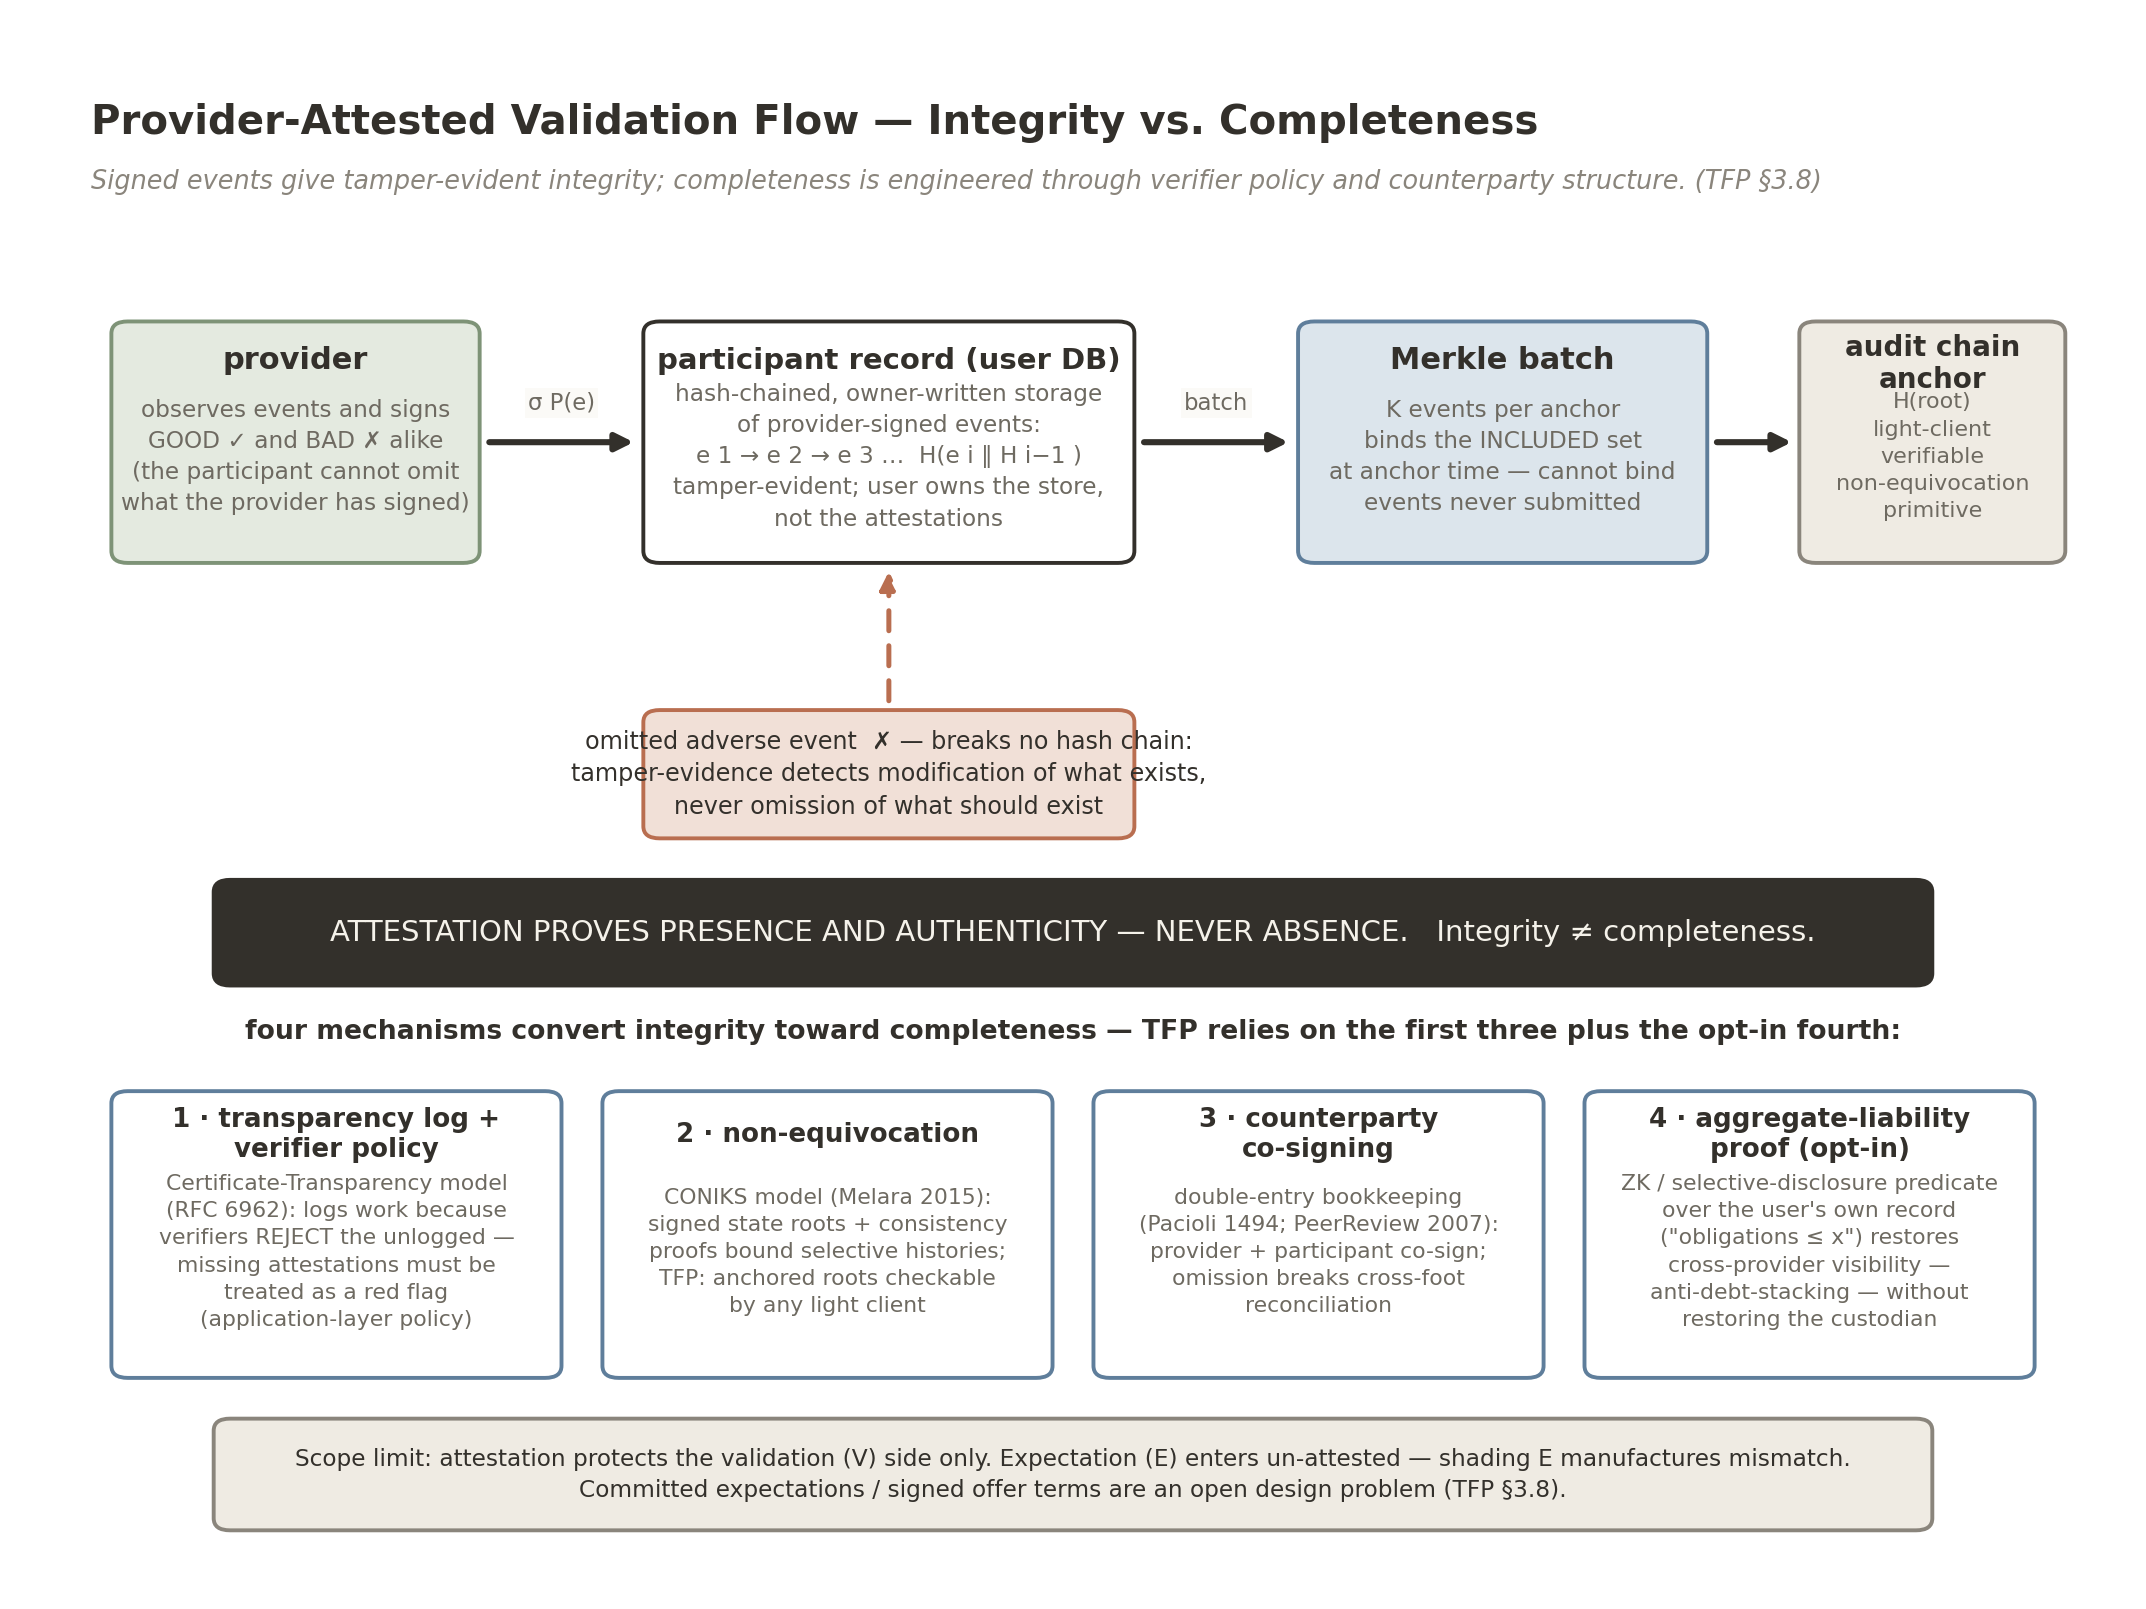
\includegraphics[width=0.92\textwidth]{figures/tfp_attestation_completeness.png}
\caption{Provider-attested validation flow and the integrity/completeness distinction (\S3.8). Providers sign good and bad events; events enter the participant's hash-chained, owner-held record, are Merkle-batched, and anchor to the audit chain. An omitted adverse event breaks no hash chain: attestation proves presence and authenticity, never absence. Four mechanisms convert integrity toward completeness --- (1) transparency log + verifier refuse-or-flag policy (Certificate Transparency, RFC 6962); (2) non-equivocation via signed state roots and consistency proofs (CONIKS); (3) counterparty co-signing (double-entry bookkeeping; PeerReview); (4) the opt-in aggregate-liability proof restoring cross-provider visibility without a custodian. Scope limit: the expectation ($E$) side is un-attested.}
\label{fig:attest}
\end{figure*}

\textbf{The design (formalized).} Validation events are
\textbf{provider-attested}: the counterparty or data provider signs the
events it observes --- good \emph{and} bad --- and the participant
cannot omit what the provider has signed, because the signed event
exists on the provider's side and is anchored to the audit chain at
signing time. Events enter the participant's record by realtime pulls
from connected accounts, each pull executed under explicit user approval
(the consent-bearing query pattern of §3.2). The participant owns the
record and the access policy; the participant does not author the
events.

\textbf{What attestation proves, precisely.} A provider-signed event
proves \emph{presence and authenticity}: this provider vouched for this
event at this time, and neither party can later repudiate or alter it
(tamper-evidence via hash-chaining; non-repudiation via the provider's
signature). It proves \textbf{nothing about absence}: neither the
provider nor the user is cryptographically prevented from omitting
events --- at the \emph{source} (the provider never writes the adverse
event) or at the \emph{aggregator} (the user connects only flattering
providers). Integrity \(\neq\) completeness; tamper-evidence detects
modification of what exists, not omission of what should exist. The
batching layer inherits the same boundary: Merkle-batch anchoring binds
the \emph{included} set at anchor time and cannot bind events never
submitted to the batch.

\textbf{Mechanisms that convert integrity toward completeness, and which
ones TFP relies on.} The literature supplies four citable designs; the
protocol's position relative to each is stated:

\begin{enumerate}
\def\labelenumi{\arabic{enumi}.}
\tightlist
\item
  \textbf{Client-side omission policy (the Certificate Transparency
  model; \citealp{rfc6962}).} CT works not because logs exist but
  because browsers \emph{reject} unlogged certificates --- completeness
  is enforced by a verifier-side policy that makes omission detectable
  and costly. TFP analogue: verifiers must treat \emph{missing} provider
  attestations as a red flag (a refuse-or-flag policy), else the log
  proves nothing about completeness. This is an application-layer policy
  requirement, stated here as a protocol-level recommendation.
\item
  \textbf{Non-equivocation and gossip (the CONIKS model;
  \citealp{melara2015}).} Signed tree roots plus consistency proofs and
  third-party auditors bound an operator's ability to show different
  observers selectively-omitted histories. TFP analogue: the audit
  chain's anchored state roots, checkable by light clients (§3.4),
  provide the non-equivocation primitive for what \emph{was} anchored.
\item
  \textbf{Counterparty co-signing (double-entry bookkeeping,
  \citealp{pacioli1494}; dual-signed accountable logs, PeerReview,
  \citealp{haeberlen2007}).} Completeness classically emerges from
  two-sided recording: omission breaks cross-foot reconciliation. TFP
  analogue: provider and participant co-sign each validation event, so a
  verifier can cross-check claimed obligations against
  counterparty-signed receipts; PeerReview demonstrates the general
  technique of detecting faulty behavior via signed, cross-checked logs.
\item
  \textbf{Regulated API completeness (the open-banking analogue; CFPB
  Personal Financial Data Rights rule, Dodd-Frank §1033, finalized
  October 2024; \citealp{cfpb2024}).} The rule requires API-based data
  sharing and bars reliance on credential screen-scraping precisely
  because scraping carries no accuracy or completeness guarantees, while
  regulated APIs carry accuracy obligations and minimum response-rate
  SLAs. Provider-side attestation in TFP is the same architectural move:
  completeness rests on (i) provider reputation and regulation, (ii)
  verifier-side policies that penalize gaps (the CT model), and (iii)
  counterparty cross-checks (the double-entry model). TFP relies on all
  three, and states so per claim type rather than claiming cryptography
  alone delivers completeness.
\end{enumerate}

\textbf{The aggregation problem: cross-provider visibility.}
Completeness has a second face that cuts against the privacy architecture and must be stated plainly: custodians also exist to give
each verifier visibility into a subject's obligations \emph{to other
verifiers}. Without cross-provider visibility, debt-stacking-style
problems re-emerge --- a subject takes on multiple near-simultaneous
obligations, each invisible to the other counterparties (the financial
quantification: loan stacking accounted for \(\sim\) \$39M of
charge-offs, \(\approx 7.8\%\) of the total, in
\citeauthor{transunion2015}'s \citeyear{transunion2015} study of the
online-lending market). Per-tenant isolation deletes this visibility by
default. The protocol's answer is an \textbf{opt-in aggregate-liability
proof}: a zero-knowledge or selective-disclosure predicate over the
participant's own record (``total current obligations \(\leq\) x''; ``no
open obligations older than y'') that a participant can present to a
verifier without disclosing the underlying events. This restores the
\emph{decision-relevant aggregate} without restoring the custodian; it
is opt-in by design, and its uptake --- hence its completeness value ---
is an application-layer and pilot-stage question, not a settled
property.

\textbf{Scope limit: the expectation side is un-attested.} Attestation
protects the validation (V) side only; expectation (E) enters
un-attested --- an agent shading E downward manufactures positive
\(\varepsilon\), and a counterparty shading E manufactures betrayal.
E-side integrity (committed expectations, signed offer terms) is an open
design problem, flagged here as a scope limit.

\textbf{Erasure on an immutable ledger (right-to-deletion
compatibility).} An append-only audit anchor raises an apparent
contradiction with erasure rights (FCRA correction/deletion duties;
GDPR Art.~17): the anchor cannot be rewritten, but the data subject's
erasure demand is binding. The protocol resolves it by keeping
content off the anchor and making erasure a key-management operation
(crypto-shredding). Concretely, each stored record is encrypted under a
three-key scheme: one key share held by the network's storage layer, one
held by the participant, and one generated per-record by the processing
service that performs validation computations. The anchor chain commits
only hashes and storage identifiers --- never content --- so destroying
the processing-service key share renders the record permanently
unrecoverable (the remaining shares are information-theoretically
insufficient) while every hash link, attestation, and state-transition
commitment on the chain remains valid and verifiable. Erasure therefore
destroys the data without breaking the ledger, and every correction or
erasure event is itself recorded on-chain as an auditable state
transition: the ledger proves \emph{that} an erasure or correction
occurred, and the audit trail of §3.4 survives it. The residual limits
match this section's general posture: erasure removes content, not the
fact of prior attestation, and derived aggregates already consumed by a
verifier are out of scope of the primitive.

\subsection*{3.9 Threat model: expected loss, not conditional exposure
{[}SIMULATION{]} + {[}EMPIRICAL
anchors{]}}

The security case of §3.6 (Sim P2) is
\emph{conditional} exposure --- records compromised given a breach. The full
risk equation is
\(E[\mathrm{loss}] = P(\mathrm{compromise}) \times \mathrm{exposure} \mid \mathrm{compromise}\),
and distribution multiplies the first term while dividing the second.
This section models both terms (Technical Appendix, Sim-Battery A, Study
2; frozen figures printed; assumptions labeled).

\textbf{Model.} \(N_{\mathrm{all}} = 3\times 10^{8}\) records in the
centralized reference (bureau-scale);
\(n_{\mathrm{devices}} = 3\times 10^{8}\) endpoints under per-tenant
custody (one per record). Expected annual attacker-exposed records:

\begin{itemize}
\tightlist
\item
  Centralized: \begin{equation} E_C = p_{\mathrm{org}} \cdot N_{\mathrm{all}}. \label{eq:ec} \end{equation}
\item
  Per-tenant: \begin{equation} E_T = n_{\mathrm{devices}} \cdot p_{\mathrm{device}} + p_{\mathrm{commonmode}} \cdot N_{\mathrm{all}}. \label{eq:et} \end{equation}
\end{itemize}

The per-tenant advantage condition reduces exactly to
\(p_{\mathrm{device}} + p_{\mathrm{commonmode}} < p_{\mathrm{org}}\):
per-endpoint compromise probability plus the common-mode failure
probability of the shared stack must stay below the organizational
breach probability. Anchors:
\(p_{\mathrm{org}} \in \{0.02, 0.03, 0.05, 0.10\}\)/yr (DBIR-class
organizational breach base rates for custodian-scale honeypots;
\citet{ibm2019} estimate a 29.6\% probability that an organization
experiences a breach within two years);
\(p_{\mathrm{device}} \in [0.001, 0.10]\)/yr (per-endpoint
phishing/malware compromise range --- real-world phishing click-through
\(\approx\) 4.1\% of delivered malicious emails, with risk concentrated
in a high-risk user quartile; human element present in 68\% of breaches,
\citealp{verizon2024});
\(p_{\mathrm{commonmode}} \in [10^{-4}, 10^{-2}]\)/yr (shared
client/supply-chain vulnerability in the per-tenant stack).

\begin{figure*}[!tp]
\centering
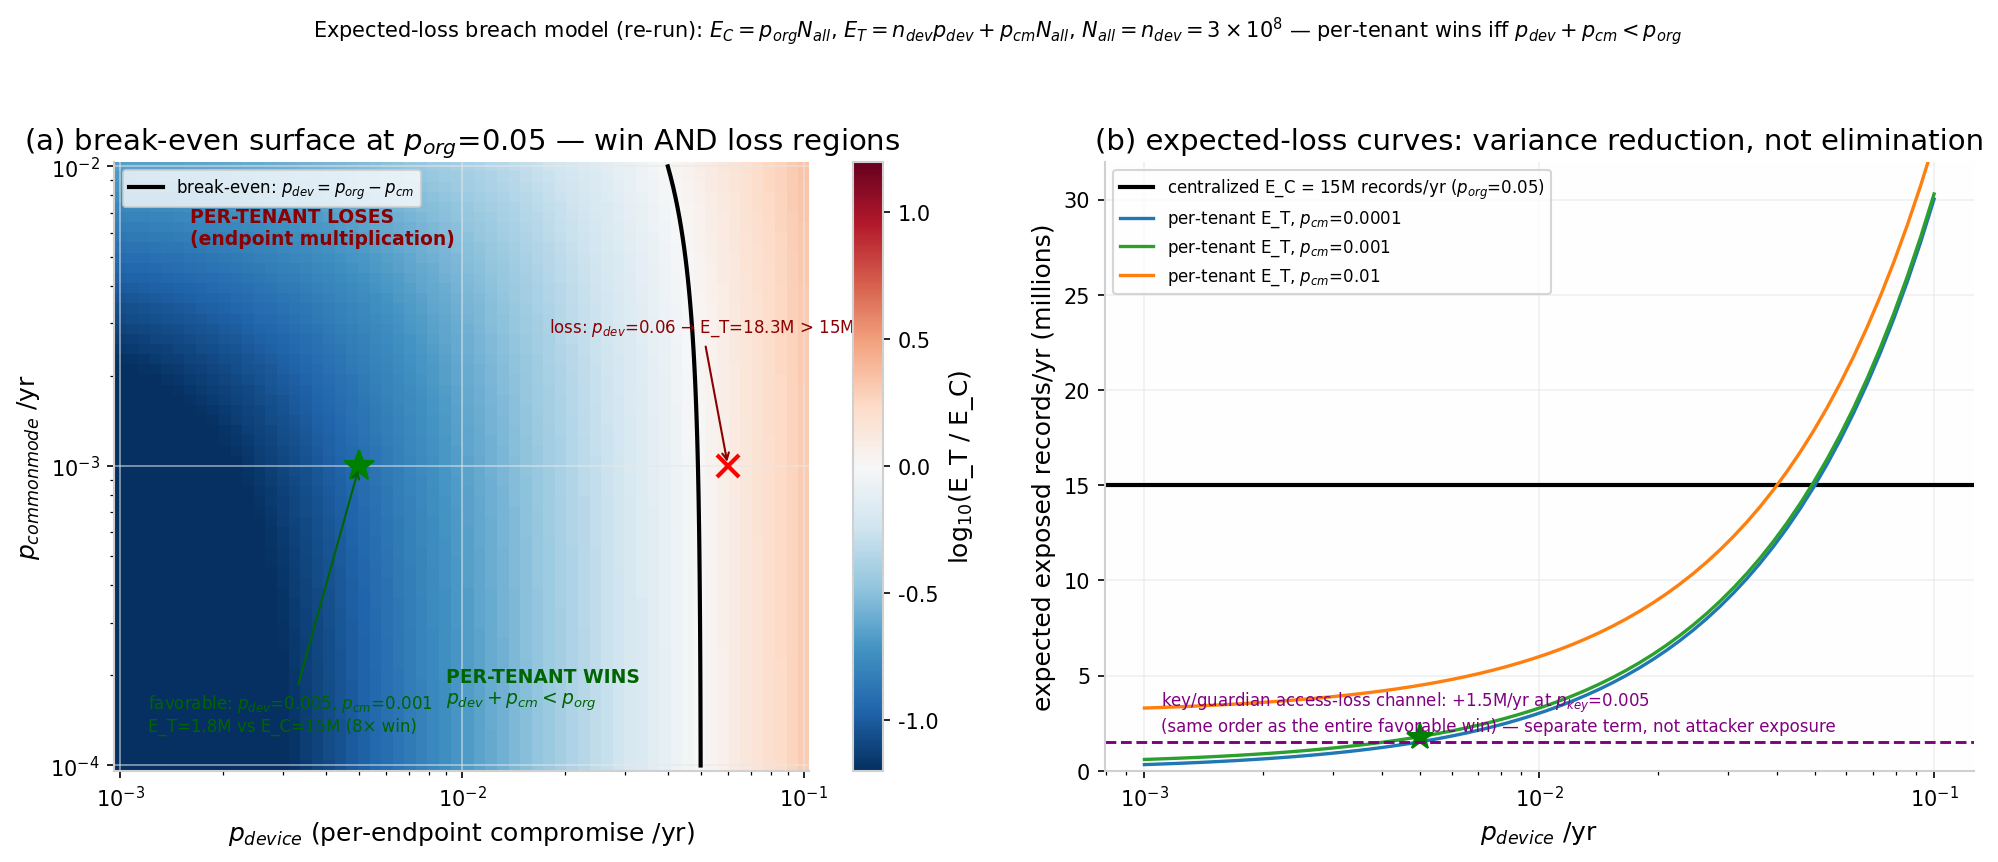
\includegraphics[width=0.92\textwidth]{figures/fig_expected_loss.png}
\caption{Expected-loss threat model (\S3.9), $N_{\mathrm{all}} = n_{\mathrm{devices}} = 3 \times 10^{8}$: (a) $\log_{10}(E_T/E_C)$ over $p_{\mathrm{device}} \times p_{\mathrm{commonmode}}$ at $p_{\mathrm{org}} = 0.05$ with the break-even contour $p_{\mathrm{device}} = p_{\mathrm{org}} - p_{\mathrm{commonmode}}$; (b) expected-loss curves --- centralized 15M records/yr at $p_{\mathrm{org}} = 0.05$; per-tenant 1.8M/yr in the favorable region ($p_{\mathrm{device}} = 0.005$, $p_{\mathrm{cm}} = 0.001$) and 18.3M/yr at $p_{\mathrm{device}} = 0.06$ --- with the key/guardian access-loss term ($+1.5$M/yr at $p_{\mathrm{key}} = 0.005$) shown separately. Variance reduction, not elimination.}
\label{fig:loss}
\end{figure*}

\textbf{Numbers (frozen, Figure \ref{fig:loss}).} Centralized expected
exposure at \(p_{\mathrm{org}} = 0.05\): \textbf{15M records/yr} (6M at
0.02; 30M at 0.10). Per-tenant \textbf{wins \(\sim 8\)\(\times\)} in the
favorable region --- \(p_{\mathrm{device}} = 0.005\),
\(p_{\mathrm{commonmode}} = 0.001 \to E_T = 1.8\)M vs.~15M --- and
\textbf{loses} when endpoint multiplication dominates:
\(p_{\mathrm{device}} = 0.06 \to E_T = 18.3\mathrm{M} > 15\mathrm{M}\);
at \(p_{\mathrm{device}} = 0.10\), \(E_T = 30\mathrm{M}{+}\) regardless
of \(p_{\mathrm{commonmode}}\). The break-even boundary is the line
\(p_{\mathrm{device}} = p_{\mathrm{org}} - p_{\mathrm{commonmode}}\).
The entire defensible region depends on per-endpoint compromise staying
well below the organizational breach rate --- plausible, because an
endpoint holds one record rather than 300M and attacker ROI per endpoint
is low, but this is an \textbf{assumption, not a measurement}, and the
market evidence cuts both ways (attackers have shifted toward individual
wallets as services hardened, \citealp{chainalysis2025}).

\textbf{Headline.} Per-tenant custody converts rare-catastrophic
loss into frequent-small loss: at \(p_{\mathrm{device}} = 0.01\)/yr and
a million tenants, \emph{some} tenant is compromised essentially every
year, while the custodian's breach is rarer and total. The
architecture's security claim is \textbf{variance reduction and
blast-radius capping --- not loss elimination} --- and it wins exactly
when endpoint hygiene and client integrity hold. Sim P2's ``99.8\%
reduction'' is retained only in its correct form: conditional exposure
given a breach, one term of the risk equation.

\textbf{Common-mode failure is a first-class scenario.} Per-tenant
isolation bounds \emph{server-side} blast radius only if tenants do not
share a monoculture client, SDK, key-derivation library, guardian
service, or update channel (\citealp{geer2003}: software monocultures
create common-mode failure). Precedents, each a case where one shared
component compromised every user of that component while the underlying
protocol stood: \textbf{Slope/Solana (August 2022;
\citealp{sentry2022})} --- a single wallet client's logging pipeline
exfiltrated seed phrases; 9,231 wallets drained in $\sim$4
hours, the Solana protocol itself unbreached; \textbf{npm event-stream
(2018)} --- a socially-engineered maintainer handoff shipped a targeted
payload to $\sim$2M-weekly-download dependents, undetected for
$\sim$2.5 months; \textbf{Ledger Connect Kit (December 2023;
\citealp{tangem2023})} --- a phished npm account pushed a wallet drainer
that dozens of applications served automatically, \(\sim\) \$600K in
under two hours; \textbf{LastPass (2022; \citealp{trm2025})} --- chained
incidents exfiltrated encrypted vault backups for $\sim$30M
users, with multi-year monetization of weak master passwords
(\(>\) \$35M traced through late 2025; \pounds 1.2M ICO fine).
Mitigations the protocol adopts as requirements, not aspirations: an
audited reference client, reproducible builds with signed releases,
update-channel key separation, and client diversity so no single client
speaks for all tenants.

\textbf{Key loss and the guardian channel --- the self-inflicted term.}
Distribution moves risk from ``a custodian loses everyone's records'' to
``users lose their keys.'' Quantified as a separate term (access loss,
not attacker exposure): at \(p_{\mathrm{key}} = 0.005\)/yr,
\textbf{+1.5M records/yr of access loss} --- \emph{the same order as the
entire per-tenant attacker-exposure win} (1.8M/yr in the favorable
example above). The counterfactual without recovery is the canonical
self-custody figure: an estimated 2.78--3.79M BTC
($\sim$17--23\% of supply) stranded in inaccessible wallets
\citep[as reported by \emph{Fortune}, 2017]{chainalysis2017}.
Guardian-quorum social recovery (ERC-4337/EIP-7702 patterns, §6;
\citealp{buterin2021}) cuts the loss channel but \textbf{adds attack
channels of its own}, each with production precedent: SIM-swap of
recovery contacts (\citealp{lee2020}: 39 of 50 attempted unauthorized
SIM swaps succeeded across five major U.S. prepaid carriers); compromise
of a centralized default guardian (\citealp{loopring2024}: \(\sim\) \$5M
across 58 wallets via the hosted 2FA guardian service); and
recovery-logic bugs (\citealp{openzeppelin2020}: a zero-guardian
recovery path put 329 wallets at immediate risk, fixed
pre-exploitation). Design requirements that follow: guardian
unlinkability, time-locked recovery with owner veto, no custodial or
default guardian as a single point, and guardian counts disclosed in the
security model. Per-tenant custody's security advantage on
attacker-exposed records is real in the favorable region --- and is
substantially offset by self-inflicted availability loss unless guardian
recovery performs much better than 0.5\%/yr.

\subsection*{3.10 Temporal validity: cold start and long-run dynamics
{[}SIMULATION{]}}

All of the stack's dynamics evidence is short-horizon; this section
reports the long-run and cold-start analyses (Technical Appendix,
Sim-Battery A, Study 1; master law with \(\lambda^{+} = 0.005,\)
\(\lambda^{-} = 0.02,\) \(\delta = 0.01\)/event,
\(S_{\mathrm{base}} = 0.5\)), which produced three findings the design
must absorb.

\textbf{(i) The update law's long-run behavior bounds the design space.}
The leak-free symmetric limit (theory preset) accumulates unbounded values
under a stationary honest stream (\(S = 249\) after \(10^{5}\) events)
--- trust inflates without bound and cross-user comparability is lost
--- while a pure leak-to-zero law erases inactive users with a 69-event
half-life (a thin-file user quiet for a quarter loses half their
standing, punishing exactly the population the cold-start story cares
about). The baseline-restoring form (\(\delta_S > 0,\)
\(S_{\mathrm{base}}\) the no-information prior --- the protocol/biological
presets) avoids both pathologies: bounded recovery after shocks (e.g., a
\(-5\) shock re-converges within 10\% of baseline in
69 events, 138/207 for \(-10\)/\(-20\)) and
an honest null worth printing --- small mismatches (\(|\varepsilon|\)
\(\lesssim 2.5\) at these parameters) are absorbed rather than scarred.

\begin{figure*}[!tp]
\centering
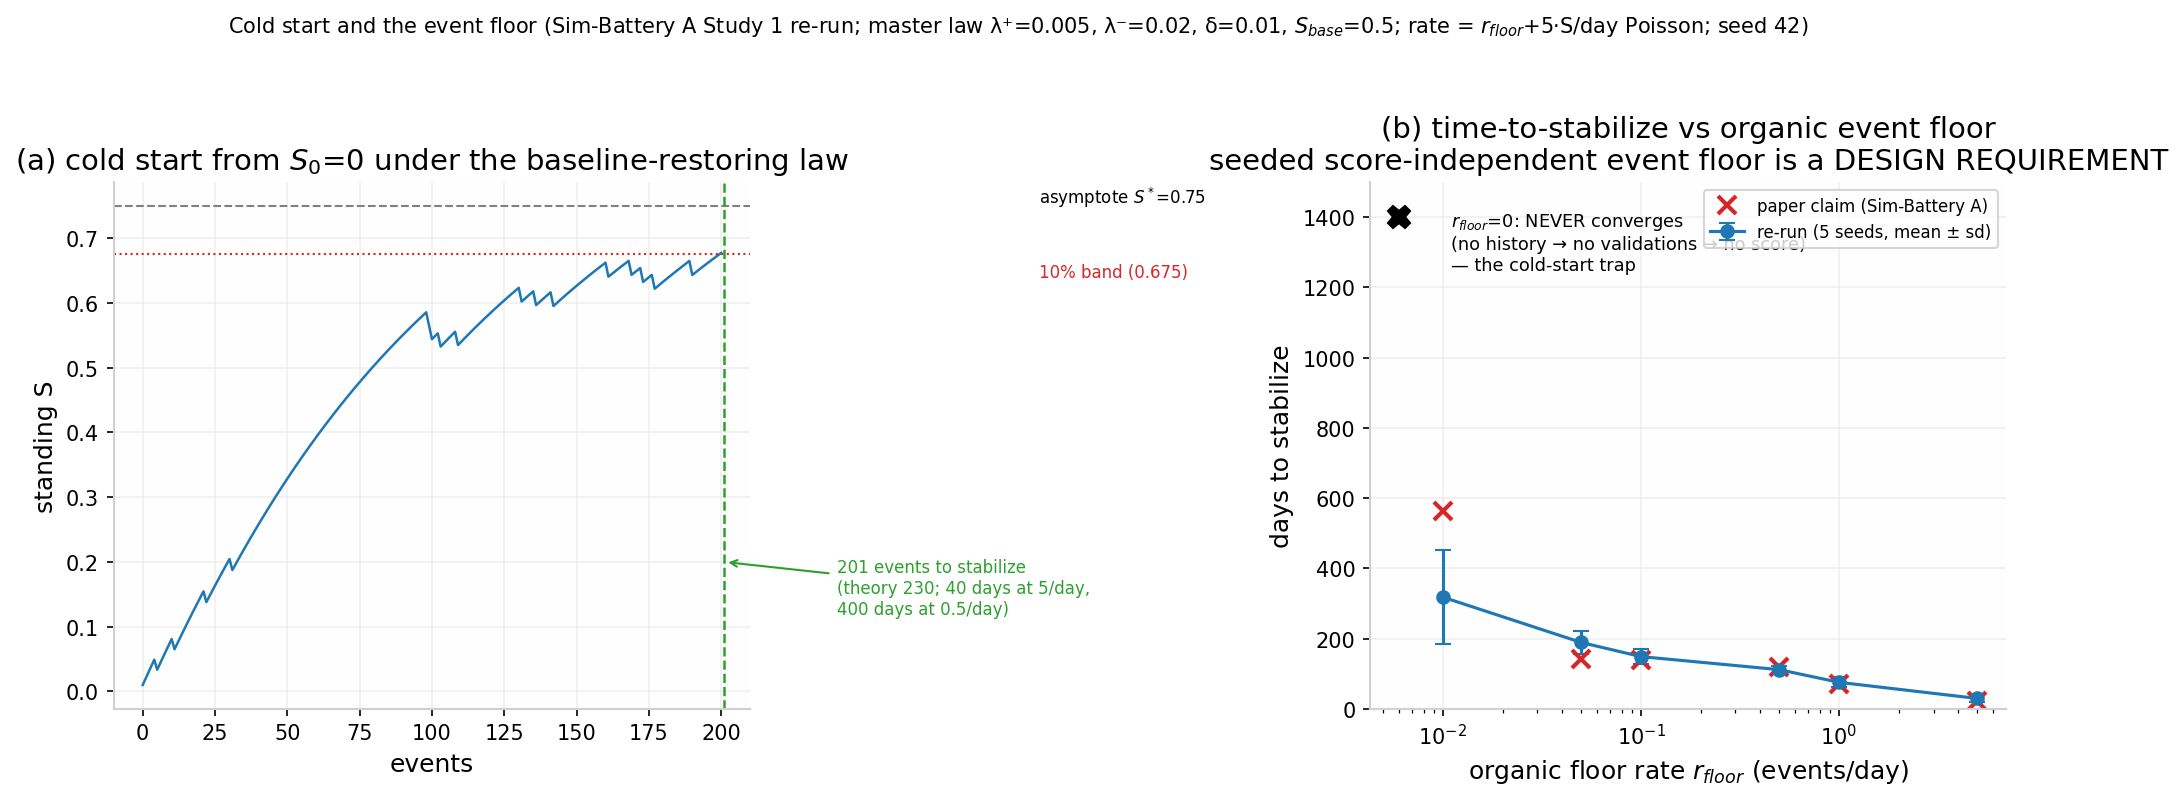
\includegraphics[width=0.92\textwidth]{figures/fig_coldstart.png}
\caption{Cold start and the event floor (\S3.10; baseline-restoring law, $\lambda^{+} = 0.005$, $\lambda^{-} = 0.02$, $\delta = 0.01$/event, $S_{\mathrm{base}} = 0.5$): from $S_0 = 0$ the law stabilizes within 10\% of the asymptote in 201 events; with rate feedback $r = r_{\mathrm{floor}} + 5S$/day, $r_{\mathrm{floor}} = 0$ never converges (the trap, exact), and escape times run $318 \pm 133$ days at $r_{\mathrm{floor}} = 0.01$/day down to 30 days at 5/day under the first-crossing criterion ($S \geq 0.9\,S^*$, $S^* = 0.75$; 189/149/112/76 days at 0.05/0.1/0.5/1 per day), with stabilization-to-asymptote at days 563/144/140/120/72/24 across the same floor grid --- both criteria verified; the earlier single-grid printing conflated them.}
\label{fig:cold}
\end{figure*}

\textbf{(ii) The cold-start trap is real, and the seeded event floor is
a design requirement, not a tunable parameter.} If event rate feeds back
from standing (rate = \(r_{\mathrm{floor}}\) + \(5\cdot S\) per day,
Poisson), then \(r_{\mathrm{floor}} = 0\) \textbf{never converges}: no
history \(\to\) no validations \(\to\) no score, permanently. Any
nonzero organic floor escapes the trap, but on very different clocks
(Figure \ref{fig:cold}). Two convergence criteria, both verified:
first-crossing ($S \geq 0.9\,S^*$, $S^* = 0.75$): day \(318 \pm 133\)
at \(r_{\mathrm{floor}} = 0.01\)/day (189/149/112/76/30 days at
0.05/0.1/0.5/1/5 per day); stabilization-to-asymptote: days
563/144/140/120/72/24 across the same floor grid. The earlier
single-grid printing conflated the two criteria; both are stated here.
From \(S_{0} = 0\) on an honest
stream, the baseline-restoring law stabilizes within 10\% of asymptote
in 201 events (theory \(\approx\) 230) --- 40 days at 5 events/day, 400
days at 0.5/day. \textbf{Design requirement:} the protocol (and any
application on it) must seed a score-independent event floor --- e.g.,
provider-initiated onboarding events --- or thin-file, low-activity
participants are trapped. This is stated as a requirement of the
architecture, not left to applications.

\begin{figure*}[!tp]
\centering
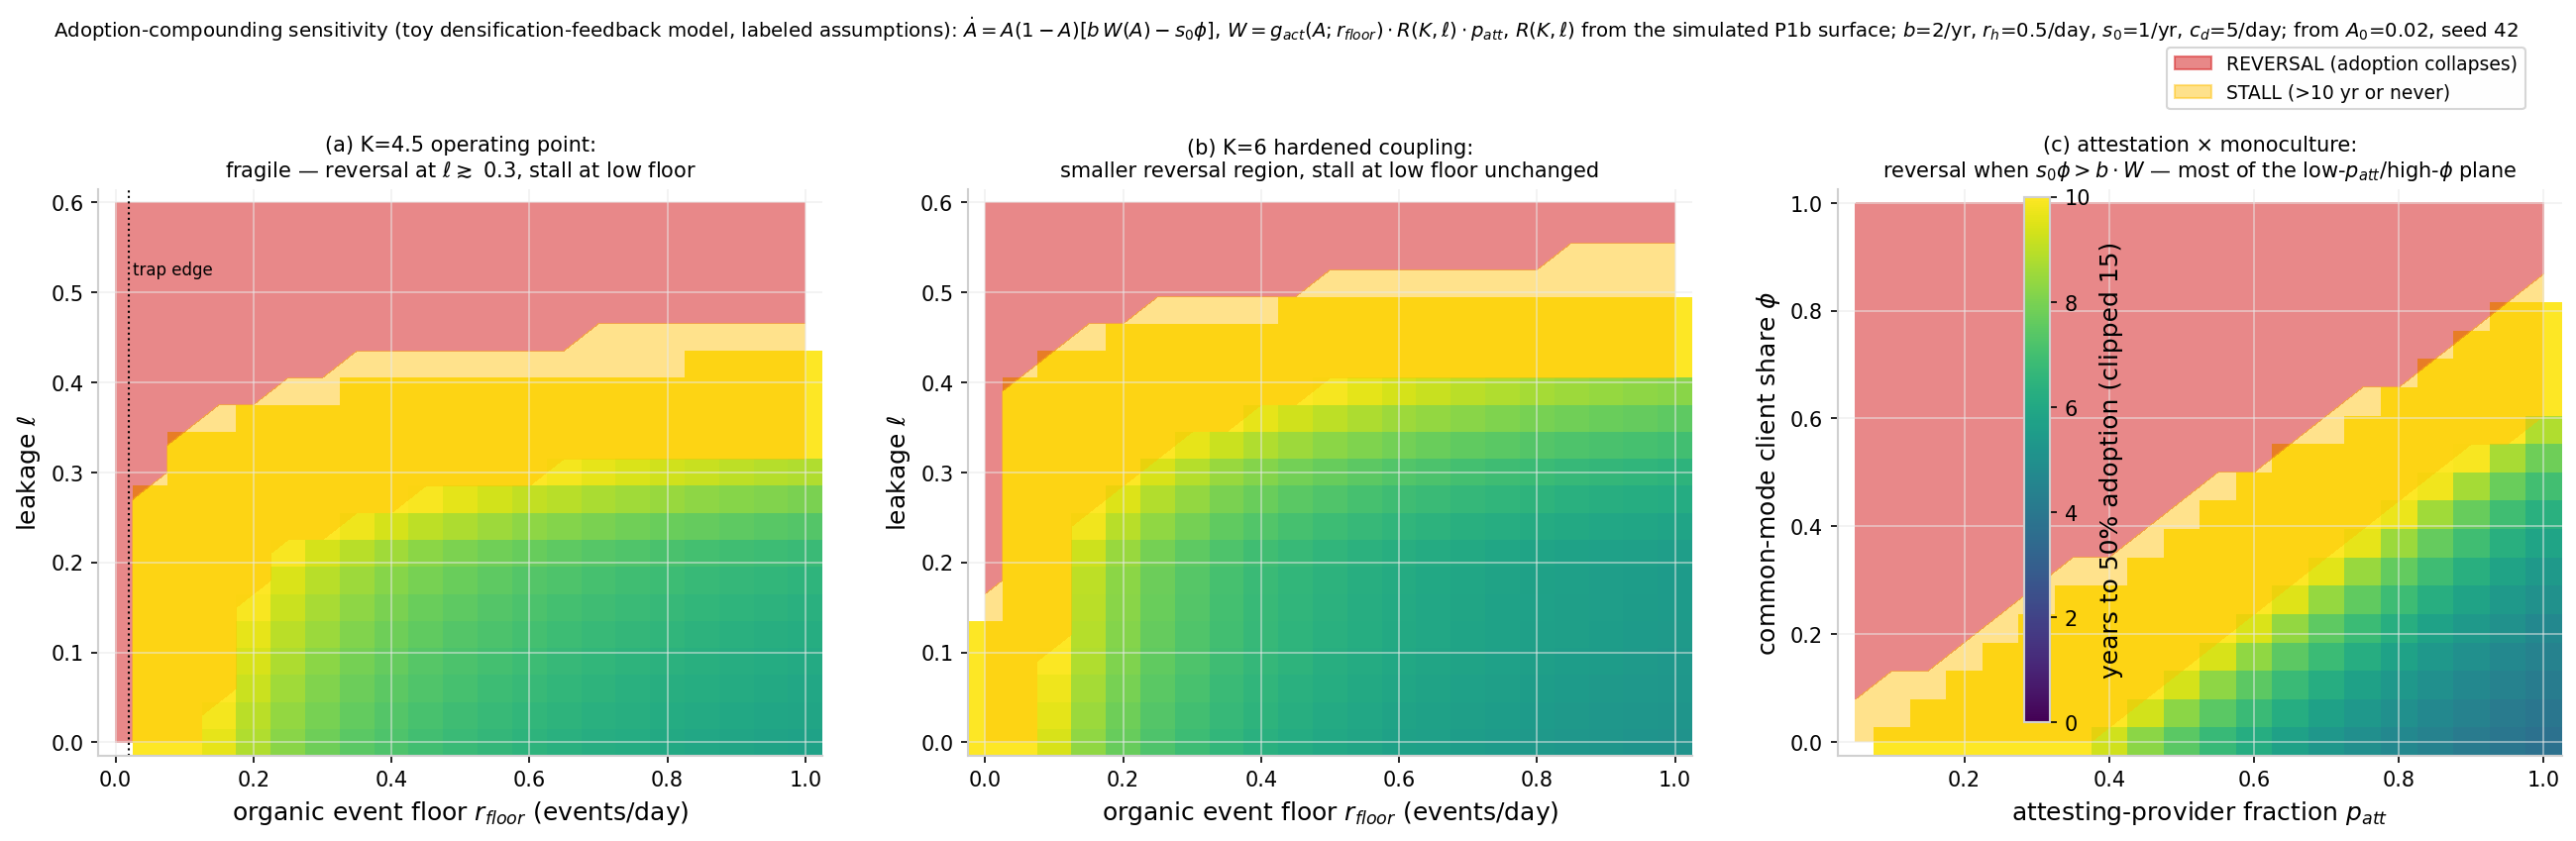
\includegraphics[width=0.92\textwidth]{figures/fig_adoption_sensitivity.png}
\caption{Adoption-compounding sensitivity (\S3.10(iii)), toy densification-feedback model of Eq.~\eqref{eq:adopt} with labeled assumptions: outcome maps over the $(r_{\mathrm{floor}}, \ell)$ plane at $K = 4.5$ (39\% compound / 28\% stall / 33\% reversal) and $K = 6$ (54\%/26\%/20\%), and over the $(p_{\mathrm{att}}, \phi)$ plane ($K = 6$, $\ell = 0.05$, $r_{\mathrm{floor}} = 0.5$). Compounding requires $r_{\mathrm{floor}} \gtrsim 0.15$/day even at $\ell = 0$, $p_{\mathrm{att}} \gtrsim 0.6$ at $\phi = 0.2$, or $\phi \lesssim 0.42$ at $p_{\mathrm{att}} = 0.8$.}
\label{fig:adopt}
\end{figure*}

\textbf{(iii) Adoption-compounding has named failure modes.} The claim
that each newly measurable participant densifies the validation graph is
a bootstrapping-phase assumption, and its failure modes are now
enumerated: the cold-start trap above (starvation at low event rates);
the leakage fragility of §3.6 (P1b: coherence at the current operating
point survives only within the band \(\ell\)* \(\in\) {[}0.02, 0.10{]}
--- early deployments with immature consent and disclosure tooling
have no measured \(\ell\); the toy model below treats \(\ell\) as an
unmeasured axis); the common-mode client risk of §3.9
(one compromised reference client during bootstrap damages every early
adopter simultaneously); and the attestation cold start (the time-floor
Sybil defense of Sim P8 only binds once providers actually attest --- a
network with few attesting providers has neither the cost multiplier nor
the time floor). Adoption compounding is therefore claimed only
conditionally: it operates once a seeded event floor, low-leakage
measurement practice, client diversity, and a minimum attesting-provider
set are in place, and each of those is an explicit deployment
precondition. A toy densification-feedback model with labeled
assumptions now quantifies each failure region (Figure \ref{fig:adopt}):
adoption follows \begin{equation} \dot{A} = A(1-A)\,\bigl[b\,W(A) - s_0\phi\bigr], \label{eq:adopt} \end{equation} with W = \(g_{\mathrm{act}}(A\);
\(r_{\mathrm{floor}})\cdot R(K\), \(\ell)\cdot p_{\mathrm{att}}\),
\(g_{\mathrm{act}}\) = r/(r + \(r_h\)), r = \(r_{\mathrm{floor}}\) + 5A
events/day, \(b = 2\)/yr, \(r_h = 0.5\)/day, \(s_{0} = 1\)/yr,
\(A_{0} = 0.02,\) and R(K, \(\ell\)) interpolated from the simulated P1b
surface. Outcomes are classified as compound (\(\leq 10\) yr to 50\%
adoption), stall, or reversal (collapse below \(0.2\cdot A_{0}\)): over
the (\(r_{\mathrm{floor}}\), \(\ell\)) plane the split is 39\%/28\%/33\%
at \(K = 4.5\) (rounding; shares sum to 100) and 54\%/26\%/20\% at \(K = 6\) --- reversal sets in for
\(\ell\) \(\gtrsim 0.30\) at \(r_{\mathrm{floor}} = 0.5\) (\(K = 4.5\))
and only for \(\ell\) \(\gtrsim 0.54\) at \(K = 6,\) while compounding
requires \(r_{\mathrm{floor}}\) \(\gtrsim 0.15\)/day even at
\(\ell = 0\) at either coupling; over the (\(p_{\mathrm{att}}\),
\(\phi\)) plane (\(K = 6,\) \(\ell = 0.05,\)
\(r_{\mathrm{floor}} = 0.5\)), compounding requires \(p_{\mathrm{att}}\)
\(\gtrsim 0.6\) at \(\phi = 0.2,\) or \(\phi\) \(\lesssim 0.42\) at
\(p_{\mathrm{att}} = 0.8.\) Hardened coupling shrinks the failure region
but does not remove the low-floor stall. The financial application preprint (specified separately) analyzes a complementary toy model (an adoption ODE with densification
coupling \(\zeta\), stalling when the organic floor \(\lesssim\)
0.01/day and \(\zeta \lesssim 0.5\) jointly); both agree compounding
requires a nonzero organic event floor and fail identically at (floor =
0, densification = 0); thresholds are model-dependent toy values, not
measurements.


\FloatBarrier
\section*{4. Observation Distortion as an Engineering
Constraint}

The protocol treats the observer effect as a design requirement in two
registers --- theoretical and empirical --- with a stated limit on what the
architecture can achieve.

\textbf{The theory, with \(\psi\) now a defined quantity {[}DERIVED for
the OU case{]}.} The theory formalizes measurement dependence as
observation-salience-dependent dissipation. Let \(m_t \geq 0\) be the
measurement-salience functional of the observation regime ---
dimensionless, increasing in (i) the subject's awareness of being
measured, (ii) the audience and persistence of the measurement record,
and (iii) the stakes attached to the record; \(m = 0\) for measurement
that is local, consent-bearing, ephemeral, and accountable. Let
\(\psi : \mathbb{R}_{\geq 0} \to \mathbb{R}\) be \(C^1\) with
\(\psi(0) = 0\) and \(\psi \geq -\mu\) (units: 1/time, same as \(\mu\)).
The mismatch process becomes

\begin{equation} d\varepsilon = -(\mu + \psi(m_t))\,\varepsilon\, dt + \sigma\, dW_t, \label{eq:ou} \end{equation}

a slow modulation of the OU drift coefficient. Sign convention:
\(\psi > 0\) is habituation (salient observation adds dissipation);
\(\psi < 0\) is hypervigilance/chilling (salient observation removes
dissipation --- the distortion regime this paper cares about). Derived
observable consequences at constant m: stationary variance
\(\sigma^2/(2(\mu + \psi))\) and autocorrelation time
\(1/(\mu + \psi)\), both diverging as \(\psi \to -\mu^{+}\) --- critical
slowing. The chilling-effects hypothesis thereby acquires a falsifiable
statistic: a surveillance-driven distortion regime shows \textbf{jointly
rising variance and rising lag-1 autocorrelation} of the mismatch
stream, a standard early-warning signature, estimable from event data
without access to anyone's state of mind.

\textbf{The \(\psi\) battery {[}SIMULATION{]}.} Technical Appendix
Sim-Battery B, Study 3, verifies the model end-to-end (exact OU
discretization, 64 parallel chains, \(\geq 30\) autocorrelation times
per run, seed 42; \(\mu = \sigma = 1\); \(\psi /\mu\) \(\in\)
{[}\(-0.95\), +1.00{]}): simulated/theory ratios for the stationary
variance within 0.8\% at all 11 grid points (at \(\psi = -0.95\mu\), Var
= 9.99 vs.~theory 10.00); lag-1 autocorrelation matching
\(e^{-(\mu+\psi)}\) within \(\pm 0.006\); dissipation-floor slowing
confirmed as variance and memory diverge \(\propto (\mu+\psi)^{-1}\);
the habituation branch verified as well (\(\psi = +1.0\mu\): Var 0.250
vs.~0.250). Distortion inflation factors relative to the unobserved
baseline: \(\psi = -0.2\mu \to \times 1.25\);
\(\psi = -0.5\mu \to \times 2.0\); \(\psi = -0.9\mu \to \times 10\).

\textbf{The limit on the architecture's own claim.} The four
architectural responses below drive salience m \(\to\)
\(m_{\mathrm{min}}\) --- but \(m_{\mathrm{min}} > 0,\) hence
\textbf{\(\psi \to \psi (m_{\mathrm{min}}) < 0,\) not 0: the protocol's
own measurement still distorts.} Measurement distortion is a parameter
shift \(\mu \to \mu\) + \(\psi (m)\), fully specified in the model; in
the field \(\psi\) enters only through \(\mu+\psi\), so the residual
level is not separately identifiable from a single stream --- the
monitoring statistic detects changes in \(\mu+\psi\) across salience
conditions (companion theory preprint, §6 H4); at an
illustrative residual salience \(\psi_{\mathrm{min}} = -0.05\mu\),
mismatch variance and memory remain inflated by \(\times 1.05\). The
architecture \emph{minimizes} observation-driven distortion; it does not
eliminate it, and no ``measurement
whose act of observing does not degrade trust'' is claimed anywhere in this
paper --- the quantified version is the claim. Two consequences are stated plainly.
\textbf{(i) Campbell's law applies to the protocol's own metrics.} The
same dynamic this paper uses against incumbents --- a measure that
becomes a target ceases to measure well --- applies to any
application-layer score computed on TFP streams: the moment a trust
readout carries stakes, salience m rises and \(\psi\) moves negative,
distorting the underlying stream. Applications must therefore treat
their own readouts as distortion-prone measurements (pre-registered
salience audits; the variance-plus-autocorrelation statistic above as
the monitoring instrument), and the protocol's design goal is restated
as keeping the residual distortion small, model-bounded, and monitored
--- not zero. \textbf{(ii) Sim P7's protective effect is double-edged in the
same currency:} the salience that lets immediate validation correct
present bias is the same salience that carries \(\psi < 0\); the net
sign is an empirical, pilot-stage question.

\textbf{Empirical register.} The chilling-effects literature shows the
distortion is large at population scale \citep{penney2016}, and
demand-characteristics research finds heterogeneous, bidirectional
participation effects with frequent nulls --- 12 of 19 studies positive,
5 clear nulls; the review concludes little is securely known about
conditions, mechanisms, or magnitudes \citep{mccambridge2014}. The
design precaution stands on the stronger Penney leg and on the generic
risk; the strong empirical claim does not. The architecture responds at four
points --- which are exactly the m-reducing conditions of the \(\psi\)
model (\(m \to m_{\min} > 0\), not \(m \to 0\)): (i) selective disclosure --- verifiers learn predicates, not
records; (ii) local-first storage --- observation requires a
consent-bearing query against the participant's own database; (iii)
accountable observation --- every access is logged where the participant
can see it; (iv) stream sequestration --- sensitive measurement streams
(e.g., physiological data used to test the biological theory) have no schema path
into application decision layers. The system thereby attempts what
centralized custodians structurally cannot: measurement whose
observation term \(\psi\) is driven to its quantified floor rather than
amplified --- with the floor, per the battery, nonzero.


\FloatBarrier
\section*{5. Protocol Evolution and
Benchmarking}

\subsection*{\texorpdfstring{5.1 V1 \(\to\) V3
evolution}{5.1 V1 \textbackslash to V3 evolution}}

The protocol has iterated through three architecture generations, each
removing a specific centralization residue:

\begin{itemize}
\tightlist
\item
  \textbf{V1 --- Sovereign storage.} Database-per-tenant edge storage
  (libSQL, single-writer per tenant by design) with user-held keys:
  eliminates the centralized data honeypot; establishes ownership
  locality.
\item
  \textbf{V2 --- Verifiable settlement.} Substrate audit layer with
  hash-anchored state transitions and Smoldot light-client verification:
  eliminates trusted-third-party record-keeping; any participant can
  verify their own record's integrity locally, without trusting an RPC
  server or other intermediary.
\item
  \textbf{V3 --- Frictionless engagement.} x402 micropayment settlement
  and edge-compiled validation compute: drives the marginal
  per-validation cost of participation toward the sub-cent floor (the
  like-for-like cost comparison of §3.6, Sim P3, with its
  events-per-decision accounting), making continuous trust measurement
  economically viable at consumer scale.
\end{itemize}

\subsection*{5.2 Benchmarking discipline: frozen figures in print,
calculator
supplementary}

Point-in-time infrastructure comparisons degrade on contact with print
(cloud pricing, chain fees, and vendor pricing all move). An earlier
version of this paper designated the live calculator at
freshcredit.xyz/cost as the canonical reference ``superseding'' static
figures; that assignment is reversed, because a mutable page on the
author's domain is not an auditable reference. \textbf{The figures
printed here are the canonical record of this paper's claims; the
calculator is a supplementary, versioned tool.} Frozen print figures
(all protocol-side quantities; incumbent comparators cited to source
where published):

\begin{itemize}
\tightlist
\item
  Per-event settlement: \$0.001/event (x402-class rails, zero protocol
  fee, sub-cent L2 gas; §3.4).
\item
  Events per application-level decision (stated assumption):
  \(10^{3}–10^{5}\), giving \$1--\$100 settlement per decision; edge
  compute on the participant's own device adds marginal electricity;
  backup storage $\sim$1 GB/tenant-year adds cents per year at
  \$0.014--0.019/GB.
\item
  The \(>\)98\% marginal-cost-reduction target (H1 leg 3) holds
  exactly when the incumbent's marginal per-query price exceeds
  \$0.05/query at equal event/query counts; incumbent marginal query
  pricing is vendor-specific and largely unpublished, so the comparison
  is maintained in the supplementary calculator with published
  assumptions and sensitivity analysis, and no static multiplier is
  asserted.
\item
  The protocol-side cost model, stated precisely: user-held data and
  user-served compute --- the participant's device executes reads,
  writes, and stability updates --- so protocol infrastructure cost per
  tenant is settlement (\$0.001/event, or \$\(10^{-7}/event\) under
  \(K = 10,000\) block rollups, §3.7) plus backup storage; there is no
  per-query toll in the protocol itself. Attestation fees charged by
  providers (the m multiplier of Sim P8) are application-layer costs,
  priced by providers, and are outside this table by design.
\end{itemize}

No achieved end-to-end performance is claimed for deployed applications.


\FloatBarrier
\section*{6. Discussion}

\textbf{What is claimed.} A composable architecture exists --- today,
from production components --- that performs trust measurement with
immediate verifiable feedback, user ownership, and distortion-minimized
observation (\(\psi\) driven to a quantified nonzero floor, §4); the
theoretical parameters it manipulates (\(\lambda\), \(\mu\), \(\psi\))
are the ones the companion theory preprint identifies as governing
trust-maintenance cost; and the failure modes of centralized
custodianship are documented at regulator-verified scale. The
collective-dynamics claims are supported in silico with their
fragilities printed (§3.6: coherence requires coupling and is fragile to
leakage at the current operating point); the security claim is an
expected-loss statement with its probability side included (§3.9:
variance reduction, conditional on endpoint hygiene and client
integrity); the cost claim is a scaling form with like-for-like
comparisons and events-per-decision accounting (§3.6, Sim P3).

\textbf{Connectome-scale simulation series.} Since the original
deposit, the collection has added a pre-registered connectome
simulation program bearing directly on the theory's neural claims: the
F1 series on the \emph{Drosophila} mushroom body (gate passed; F1a
INDETERMINATE-instrument; F1a2 FAIL on its control-shuffle criterion;
F1b compartment-resolved gating PASS (7/7 as frozen; criteria 6--7 met at a floor-saturation calibration artifact, evidential weight on 1--5) --- reported in full, with
the KC share of MBON input budget measured at 0.982) and Simulation H1
on MICrONS mouse cortex (structural dominance FAIL; permutation
robustness MET; compound verdict FAIL), with a human-cortex
replication (H01) pre-registered and in progress. These results are
reported where they belong --- in the companion biological-instantiation preprint (\S{}5.6--5.7, the
F1-series and H1 subsections) --- and
are summarized in the collection index. This paper's protocol claims do
not depend on any of them; the pointer is provided so that readers
following the theory's biological motivation can find the
connectome-scale evidence, including its failures, in one place.

\textbf{What is not claimed.} No domain application, no achieved
end-to-end performance, no static cost multiplier, no decision logic of
any kind --- all of that lives in application documents such as the financial application preprint (specified separately). No claim that observation distortion is eliminated
(it is minimized and monitored). No claim that per-tenant custody
reduces \emph{expected} loss unconditionally (it caps blast radius and
reduces variance; §3.9). No protocol-level governance mechanism (§3.5).
No defense against coordinated collusion rings (below). No data-custody
cascade model (DebtRank is a category error for data custody; no such
literature exists --- stated as a gap, §3.7 Sim P6).

\textbf{Principal limitations.} (i) Demonstrated chain throughput is
network-level, not application-level (and the headline figure is for
batch transactions; §3.4); realized per-user latency depends on indexing
and edge topology. (ii) The chilling-effects evidence is drawn from
surveillance contexts; its generalization to commercial measurement is
plausible but unproven --- itself a testable prediction of the stack, in
the falsifiable form of §4's joint variance/autocorrelation statistic.
(iii) Database-per-tenant shifts the operational burden (key management,
recovery) onto participants, and the quantified size of that channel is
the same order as the security win (§3.9). The account-layer solution
pattern now exists in production and TFP adopts it by reference rather
than reinventing it: smart-account standards (ERC-4337, deployed 2023;
EIP-7702, live with Ethereum's 2025 Pectra upgrade;
\citealp{buterin2021}) provide guardian-quorum social recovery, scoped
session keys, and key rotation --- recovery and delegation without
reintroducing a custodian --- while passkey signers (WebAuthn) replace
seed-phrase custody with device biometrics. The residual risk moves from
``a custodian loses everyone's records'' to ``a user loses their
guardians'' --- with the guardian channel's own documented attack
surfaces (SIM-swap, guardian-service compromise, recovery-logic bugs;
§3.9) now part of the threat model, and key rotation converting a stolen
key from a permanent identity loss into a revocable event. (iv) Temporal
validity: the cold-start trap is real and the seeded event floor is a
design requirement (§3.10); long-run behavior is bounded only under the
baseline-restoring presets. (v) Sim P7's protective effect was measured
at one salience setting; the salience-parameter sensitivity analysis is
registered future work (§3.7). (vi) The \(\psi\) floor is nonzero (§4):
the protocol's own measurement distorts, and applications inherit a
Campbell's-law obligation.

\textbf{Adversarial robustness.} Trust and reputation systems face a
standard attack taxonomy --- on-off, badmouthing, self-promoting,
whitewashing, Sybil, oscillation, and RepTrap attacks
\citep{hoffman2009,jalaly2023} --- and TFP's mitigations are structural
rather than algorithmic. The supportable version of each:
\textbf{Sybil identity creation} \citep{douceur2002} is \emph{not}
bounded by settlement cost alone --- \$1.01 buys 10 units of unattested
standing at the protocol's own per-event figures; the real defense is
provider attestation (a linear cost multiplier m) combined with the
wall-clock time floor, quoted per rate (1,005 attested events: at
\(\leq 2\)/day, 1.4 years; at the model's own high-standing rates of
2.5--3.76 events/day, \(\sim\)0.55--1.1 years at 2.5--5/day (0.73 yr at 3.76/day; 0.55 yr at 5/day); at the decisionable
threshold of \(\sim\)60--70 events, \(\sim\)72 days with one
cooperative provider), with block rollups cutting honest cost \(10^{4}\times\)
without relaxing the time floor, and with the
parallel-provider-collusion caveat disclosed (§3.7, Sim P8).
\textbf{Whitewashing} is bounded because absence of history is itself
measurable --- a fresh record starts at the prior, not at a clean high
standing, and rebuilding costs real \emph{attested} events over real
time --- and because the completeness mechanisms of §3.8 make
selectively-curated histories detectable at the verifier's policy layer.
\textbf{On-off and oscillation attacks} are bounded by the same
immediate-feedback property that makes measurement honest: behavior
updates the record at event time, so slowly built trust cannot be spent
in a single unpunished burst (under the explicit
\(\lambda^{-} > \lambda^{+}\) preset; re-run registered, §3.7).
\textbf{Manufactured-history markets} exist in the incumbent world too
--- tradeline renting sells seasoned authorized-user slots at
\$325--\$4,000+ (FTC enforcement record), and synthetic identities are
seasoned for months-to-years before bust-out (Federal Reserve
white-paper series, \citeyear{fed2019}) --- so the time-floor defense is
aimed at a documented attack economy, not a hypothetical one. The residual is coordinated collusion (RepTrap, badmouthing rings):
selective disclosure limits the information attackers can coordinate on,
but the literature is clear that no defense guarantees complete
prevention and that defenses trade off against each other
\citep{jalaly2023} --- collusion-ring detection remains an open problem,
stated as one. The 20\% adversarial event rate in the §3.6 population
run and the Sim P8 attack battery (§3.7, Supporting Document §R) are the
simulation-level instantiations of this concern. Resilience at
production scale, and collusion-ring behavior specifically, are
pilot-stage empirical questions.

\textbf{Claims-to-evidence map.} Every load-bearing claim in this paper,
its epistemic label, and where its support lives. C1--C2 are inherited
from the companion theory preprint and restated here because every downstream claim stands on them; they are derived and numerically verified there, not in this paper. C3--C17 are this paper's own claims.


\begin{table*}[t]
\centering
\caption{Claims-to-evidence map. Every load-bearing claim, its epistemic label, and where its support lives. C1--C2 are inherited from the companion theory preprint and restated because every downstream claim stands on them; C3--C17 are this paper's own claims.}
\label{tab:claims}
\scriptsize
\setlength{\tabcolsep}{4pt}
\begin{tabular}{@{}l p{4.35cm} p{2.3cm} p{3.95cm} p{5.35cm}@{}}
\toprule
\# & Claim & Label & Evidence & Status \\
\midrule
C1 & Trust-vector dynamics converge to a stable alignment manifold under the stability law & [DERIVED] + [SIMULATION] & companion theory preprint, \S3.2 (Lyapunov); Sim G1 & Verified analytically and numerically (symmetric leak-free limit; extensions preserve stability per branch) \\
C2 & Populations phase-lock toward PAS coherence at moderate coupling; $K_c = 2/(\pi g(0))$ is the mean-field reference & [ANALOGY] (functional form) + [SIMULATION] (behavior of the analogy in mean field; the threshold is derived within the Kuramoto model only) & companion theory preprint, \S3.4 (Kuramoto); Sim G1 & Verified in mean field; $K_c$ restated as a reference value with assumptions, not a prediction \\
C3 & Coupling produces collective coherence; isolation remains incoherent (Sim P1) & [SIMULATION] & \S3.6: $R = 0.739 \pm 0.029$ ($K = 4.5$) vs.\ $0.040 \pm 0.001$ ($K = 0$, at the $1/\sqrt{N}$ floor) & Supported in silico (verification re-run); control baseline at the $1/\sqrt{N}$ floor under the stereographic phase map; pilot test open \\
C4 & Observation leakage degrades coherence monotonically (Sim P1b) & [SIMULATION] & \S3.6: $R(K, \ell)$ surface; at $K = 4.5$, $R = 0.709 \to 0.041$ across $\ell = 0 \to 0.9$ & Mechanism supported; \textbf{honest null}: $R > 0.7$ at $K = 4.5$ survives only within the band $\ell^* \in [0.02, 0.10]$; robust claim needs $K = 6$ ($\ell \approx 0.22\text{--}0.28$) or $K = 8$ ($\ell \approx 0.30\text{--}0.40$) \\
C5 & Per-tenant isolation reduces single-breach conditional exposure by $\geq 98\%$ (Sim P2) & [SIMULATION] + architectural argument & \S3.6 Monte-Carlo breach comparison & Supported \emph{conditional on breach}; expected-loss reframing with probability side in \S3.9 (C14) \\
C6 & Per-event settlement scales at constant marginal cost; per-decision cost is \$1--\$100 at $10^3$--$10^5$ events (Sim P3) & [SIMULATION] of scaling form + frozen print figures & \S3.6; \S5.2 & Scaling form supported; like-for-like marginal comparisons only; $>$98\% reduction conditional (incumbent marginal query cost $>$ \$0.05/query) \\
C7 & Model-predicted (battery-derived) heterogeneity preserves collective coherence (Sim P4a) & [SIMULATION] & \S3.6 cross-layer seeded run, $R = 0.759 \pm 0.024$ & Supported in silico (caveat recorded: phase dynamics are $\lambda$-independent in the current ABM) \\
C8 & Model-predicted (battery-derived) heterogeneity leaves a detectable but practically negligible footprint (Sim P4b) & [SIMULATION] & \S3.6: battery-seeded energy distance 0.00021, $p = 0.005$; lower-powered seeding $p = 0.109$ (null) & Seeding variable shown non-inert, effect size negligible; the lower-powered null is preserved in the record \\
C9 & Distortion-minimizing observation is achievable in production --- with $\psi \to \psi_{\min} < 0$, not 0 & [HYPOTHESIS] + [DERIVED] (OU limits) + [SIMULATION] & \S4 design argument; $\psi$ battery ($\times 1.05$ inflation at $\psi = -0.05\mu$); chilling-effects literature & ``Quantified minimization claimed ($\psi \to \psi_{\min} < 0$), not
  elimination; Campbell's-law obligation stated for the protocol's own metrics; field validation open \\
\bottomrule
\end{tabular}
\end{table*}


\begin{table*}[t]
\centering
\caption{Claims-to-evidence map, part 2 (C10--C17; continued from Table~\ref{tab:claims}).}
\label{tab:claims2}
\scriptsize
\setlength{\tabcolsep}{4pt}
\begin{tabular}{@{}l p{4.35cm} p{2.3cm} p{3.95cm} p{5.35cm}@{}}
\toprule
\# & Claim & Label & Evidence & Status \\
\midrule
C10 & Bilateral validation is informationally symmetric; surveillance is one-directional (Sim P5) & [SIMULATION] & \S3.7, surrogate-corrected transfer entropy: $0.0315 \pm 0.003$ / $0.0283 \pm 0.002$ bits both directions; surveillance $0.121 \pm 0.005$ / $-0.001 \pm 0.001$ & Directions supported (all replicas on the correct side of the threshold); magnitudes floor-adjacent, so no ratio is claimed; per-replica CIs registered as a re-run requirement; the biased estimator is documented in \S{}Q.3 \\
C11 & Per-tenant isolation bounds cascade reach by construction (Sim P6) & Architectural argument & \S3.7: zero-edge topology admits no propagation channel & No cascade model applied to data custody (DebtRank is a category error there); no data-custody cascade literature exists --- gap stated; quantitative security claim moved to C14 \\
C12 & Immediate validation reduces adversarial-contract uptake by present-biased agents (Sim P7) & [SIMULATION] & \S3.7 $\beta\delta$-agent battery: uptake $0.725 \to 0.284$, $p = 0.004$ & Supported in silico at one salience setting; salience-parameter sensitivity analysis absent --- stated limitation, re-run registered; field analogue is a pilot hypothesis \\
C13 & The population model reproduces the heavy-tailed event-outcome stylized fact (Sim P5b) & [SIMULATION] & \S3.7, excess kurtosis 1.9 on L1 reallocations & Supported; measured on L1 reallocations (an on-simplex measure is identically zero, \S Q.4) \\
C14 & Expected-loss security: per-tenant custody wins iff $p_{\mathrm{device}} + p_{\mathrm{commonmode}} < p_{\mathrm{org}}$; key/guardian loss is the same order as the win & [SIMULATION] + [EMPIRICAL] anchors & \S3.9: 15M/yr centralized ($p_{\mathrm{org}} = 0.05$) vs.\ 1.8M/yr per-tenant ($p_{\mathrm{device}} = 0.005$, $p_{\mathrm{cm}} = 0.001$), 18.3M at $p_{\mathrm{device}} = 0.06$; $+1.5$M/yr access loss at $p_{\mathrm{key}} = 0.005$ & Supported as a model with labeled assumptions; headline: variance reduction, not elimination; common-mode precedents cited (Slope, event-stream, Ledger Connect Kit, LastPass) \\
C15 & Canonical reputation attacks (Sybil, whitewashing, on-off) are structurally dominated under the protocol's update rule (Sim P8) & [SIMULATION] & \S3.7, Supporting Document \S R: linear Sybil cost; repair $>$ whitewash at $d \leq 8$ (tied at $d = 16$ under the bare standing metric); on-off dominated under immediate feedback & Supported in silico; manufactured standing is cheap without attestation (\$1.01/10 units unattested); real defense = attestation multiplier + rate-dependent wall-clock time floor (1.4 yr at $\leq$2/day; $\sim$0.55--1.1 yr at the model's own high-standing rates, 0.73 yr at 3.76/day and 0.55 yr at 5/day); whitewash dominance at $d = 16$ requires the \S3.8 verifier-side fresh-record flag; rollups decouple honest cost; parallel-collusion caveat disclosed; $\lambda^{-} > \lambda^{+}$ preset now explicit in specification; P8 verification re-run under the explicit preset pending (registered) \\
C16 & Provider attestation proves presence/authenticity of signed events, not completeness; completeness rests on verifier policy (CT model), non-equivocation (CONIKS model), and counterparty co-signing (double-entry/PeerReview model) & [STANDARD] + design argument & \S3.8; \citealp{rfc6962}; \citealp{melara2015}; \citealp{haeberlen2007}; \citealp{cfpb2024} & Stated with precise logical limits; opt-in aggregate-liability proof specified for cross-provider visibility (debt-stacking: \citealp{transunion2015}, $\sim$\$39M charge-offs); uptake is a pilot question \\
C17 & Cold-start trap is real; a seeded score-independent event floor is a design requirement & [SIMULATION] & \S3.10: $r_{\mathrm{floor}} = 0$ never converges; day-318 at 0.01/day vs.\ day-30 at 5/day (criterion $S \geq 0.9 S^*$) & Supported in silico (verification re-run); adopted as an architectural requirement; adoption-compounding claim conditioned on named preconditions \\
\bottomrule
\end{tabular}
\end{table*}


The claims table deliberately preserves the full evidential history ---
C8's null under the first seeding alongside support under the better-powered
one, the failed estimators inside C10 and C13, and the C4 honest
null. This is methodological: the claims table is the audit surface, and a
stack that reports only its successes cannot be audited.


\FloatBarrier
\section*{7. Conclusion}

Trust measurement is infrastructure, and the incumbent infrastructure
centralizes custody, delays feedback, and distorts its subjects. The
Fresh Protocol specifies the alternative the theory calls for ---
immediate, verifiable, user-owned validation --- as a domain-agnostic
stack built from components whose individual performance is already
demonstrated. This revision has narrowed the claims to what the evidence
carries: coherence is produced by coupling and is fragile to observation
leakage at the current operating point; distribution caps blast radius
and reduces variance rather than eliminating expected loss; attestation
proves presence, and completeness is engineered through verifier policy
and counterparty co-signing rather than assumed from cryptography; the
protocol's own measurement distorts, at a quantified floor; and the cost
advantage is a scaling form with like-for-like accounting, not a
headline multiplier. The protocol specifies no domain semantics; the
interpretation of any measured stream is assigned exclusively to
application-layer specifications.


\FloatBarrier
\section*{Notes on the record}

\textbf{Removed from the reference list:} Thomson Reuters Institute
(2023), \emph{Trends in synthetic identity fraud} --- the ``95\% of
synthetic identities pass onboarding undetected'' figure attributed to
it could not be traced to any primary report, methodology, or date
(circular vendor citation); the claim is marked unverifiable in §1.1 and
replaced by the Federal Reserve white-paper series.

Live benchmarks:
freshcredit.xyz/cost (versioned cost/speed/security comparisons ---
supplementary tool; the print figures of §5.2 are canonical for this
paper's claims). Simulated results are labeled as such wherever they
appear; no production performance is claimed.

\textbf{Epistemic labels used in this paper:} {[}DERIVED{]} (follows
from stated assumptions), {[}STANDARD{]} (textbook results derived for
self-containment), {[}ANALOGY{]}, {[}HOMOLOGY{]}, {[}EMPIRICAL{]},
{[}HYPOTHESIS{]}, {[}SIMULATION{]}.

\textbf{Competing interests:} D.S. is the founder and a beneficiary of FreshCredit Inc. and the
founder of The FreshCredit Lab.~FreshCredit Inc holds granted US utility
patents covering methods in three commercial verticals (finance,
commerce, and insurance): US 12,236,480 B2; US 12,293,410 B2; US
12,307,515 B2; US 12,293,411 B2 (grant statuses per public records;
recorded assignment to FreshCredit, April 4, 2025); the
underlying protocol is otherwise open. The patents list Devon Shigaki as
inventor/applicant. The theoretical results and the
patented methods overlap in composition; the author discloses this
overlap explicitly.

\textbf{Acknowledgments:} AI assistants (Kimi K3, Moonshot AI; Claude
Fable 5, Anthropic) contributed to validation, adversarial
review, and simulation code. All original ideas, claims, and conclusions are
the author's own.

\textbf{Data availability:} Simulation code, seeds, figures, and pre-registration documents are deposited at OSF (DOI: [insert]). The Supporting Document and Technical Appendix are in preparation (see collection index); until they are deposited, the frozen-criteria and protocol claims that cite them are self-attested. Benchmark figures cited in print are frozen snapshots; the
live calculator at freshcredit.xyz/cost is a supplementary tool, not a
reference. 

\textbf{Funding:} none received; independent research. \textbf{Author
contributions:} D.S. is the sole author and is responsible for all
content.

\bibliographystyle{plainnat}
\bibliography{tfp}

\end{document}
